% ----------------------------------------------------------------------
%                   LATEX TEMPLATE FOR PhD THESIS
% ----------------------------------------------------------------------

% based on Harish Bhanderi's PhD/MPhil template, then Uni Cambridge
% http://www-h.eng.cam.ac.uk/help/tpl/textprocessing/ThesisStyle/
% corrected and extended in 2007 by Jakob Suckale, then MPI-CBG PhD programme
% and made available through OpenWetWare.org - the free biology wiki
% Modified to conform with University of Pennsylvania Thesis Requirements 
% by Alan Meert & David F. Moore, 2013, Dept. of Physics and Astronomy

%: --------------------------------------------------------------------------
%: Style file for Latex
%: Specify openright if printing double-sided, openany if single-sided
%: --------------------------------------------------------------------------
\documentclass[11pt, openany, oneside]{Latex/Classes/PhDthesisPSnPDF}
\usepackage{lipsum} % this just creates filler text when needed

%: --------------------------------------------------------------------------
%: Use Natbib for non-standard citations 
%: --------------------------------------------------------------------------
%: uncomment below to change from standard TeX in-text citations to
%: author-year in-text citations. Should be used together with the 
%: PhDbiblio-intext-twoauth.bst file (included with this project) or 
%: some other acceptable .bst file 
%: --------------------------------------------------------------------------

%\usepackage[authoryear]{natbib}
%  \bibpunct{(}{)}{;}{a}{}{,}

%: --------------------------------------------------------------------------
%: The end user may modify these files to personalize and define macros
%: --------------------------------------------------------------------------
\usepackage{Latex/StyleFiles/UserDefs} % Define any user-defined Macros and functions in this file.
% This file contains macros that can be called up from connected TeX files
% It helps to summarise repeated code, e.g. figure insertion (see below).

% insert a centered figure with caption and description
% parameters 1:filename, 2:title, 3:description and label
\newcommand{\figuremacro}[3]{
	\begin{figure}[htbp]
		\centering
		\includegraphics[width=1\textwidth]{#1}
		\caption[#2]{\textbf{#2} - #3}
		\label{#1}
	\end{figure}
}

% insert a centered figure with caption and description AND WIDTH
% parameters 1:filename, 2:title, 3:description and label, 4: textwidth
% textwidth 1 means as text, 0.5 means half the width of the text
\newcommand{\figuremacroW}[4]{
	\begin{figure}[htbp]
		\centering
		\includegraphics[width=#4\textwidth]{#1}
		\caption[#2]{\textbf{#2} - #3}
		\label{#1}
	\end{figure}
}

% inserts a figure with wrapped around text; only suitable for NARROW figs
% o is for outside on a double paged document; others: l, r, i(inside)
% text and figure will each be half of the document width
% note: long captions often crash with adjacent content; take care
% in general: above 2 macro produce more reliable layout
\newcommand{\figuremacroN}[3]{
	\begin{wrapfigure}{o}{0.5\textwidth}
		\centering
		\includegraphics[width=0.48\textwidth]{#1}
		\caption[#2]{{\small\textbf{#2} - #3}}
		\label{#1}
	\end{wrapfigure}
}

% predefined commands by Harish
\newcommand{\PdfPsText}[2]{
  \ifpdf
     #1
  \else
     #2
  \fi
}

\newcommand{\IncludeGraphicsH}[3]{
  \PdfPsText{\includegraphics[height=#2]{#1}}{\includegraphics[bb = #3, height=#2]{#1}}
}

\newcommand{\IncludeGraphicsW}[3]{
  \PdfPsText{\includegraphics[width=#2]{#1}}{\includegraphics[bb = #3, width=#2]{#1}}
}

\newcommand{\InsertFig}[3]{
  \begin{figure}[!htbp]
    \begin{center}
      \leavevmode
      #1
      \caption{#2}
      \label{#3}
    \end{center}
  \end{figure}
}


%%% Local Variables: 
%%% mode: latex
%%% TeX-master: "~/Documents/LaTeX/CUEDThesisPSnPDF/thesis"
%%% End: 
 % Some prewritten Macros for Use in Latex

\usepackage[T3]{fontenc}
\usepackage{charter}
\usepackage[expert]{mathdesign}

%: ----------------------------------------------------------------------
%:                  User information
% -----------------------------------------------------------------------

% DISSERTATION TITLE
\title{Mapping Functional Architecture in Neocortical Epileptic Networks} %The title of your thesis
% Optional Sub-title
%\SubTitle{Mapping Epileptic Networks} %comment if you don't want a subtitle

%YOU 
\author{Ankit Narendra Khambhati}

% Degree information
\DegreeDate{2015} % expected year of graduation.
\degree{Doctor of Philosophy}

%YOUR DEPARTMENT and UNIVERSITY
\collegeordept{Bioengineering}
\university{University of Pennsylvania}

%YOUR ADVISOR
\supervisor[Professor of Neurology \& Bioengineering]{Brian Litt}

% Your Department Graduate chair
\gradchair[Professor of Bioengineering]{Jason Burdick}

% Additional Commitee Members [title]{Name}
\firstcomittee[Professor of Electrical and Systems Engineering \& Computer and Information Science]{Daniel D. Lee}
\secondcomittee[Skirkanich Assistant Professor of Innovation of Bioengineering]{Danielle S. Bassett}
\thirdcomittee[Assistant Professor of Neurosurgery, Perelman School of Engineering]{Timothy H. Lucas}


% Copyright statement of your choice
\CopyrightStatement{This work is licensed under the Creative Commons
Attribution-NonCommercial-ShareAlike 4.0 License.\newline
\noindent To view a copy of this license, visit
\href{http://creativecommons.org/licenses/by-nc-sa/4.0/}{%
http://creativecommons.org/licenses/by-nc-sa/4.0/}
}

%: --------------------------------------------------------------
%:                  BEGIN THE DOCUMENT!!!
% --------------------------------------------------------------
\begin{document}

% sets line spacing
\renewcommand\baselinestretch{1.2}
\baselineskip=18pt plus1pt

%: ------------------------------------------------------------------------
%:                  FRONT MATTER: dedications, abstract,..
% -------------------------------------------------------------------------

%: ----------------------- generate cover page ----------------------------
\maketitle  

%: ----------------------- generate copyright page ------------------------
\makecopyright  

%: ----------------------- Include a Dedication ---------------------------
% Thesis Dedictation ---------------------------------------------------

\begin{dedication} %this creates the heading for the dedication page

\large\emph{To Baa, \\ \indent for her strength, \\ and Dada, \\ \indent for his resolve.}

\end{dedication}

% ----------------------------------------------------------------------


%: ----------------------- Include an Acknowledgement ---------------------
% Thesis Acknowledgements ------------------------------------------------

\begin{acknowledgements}
Five years ago, the opportunity to conduct meaningful and clinically impactful brain research seemed a far off pipe dream. First and foremost, I thank my advisor and mentor, Brian Litt, for placing his trust in me and inviting me to pursue Master's and Doctoral-level research. Brian, I am indebted to you for showing me how to ask big-picture questions and instilling in me the grander vision of conducting research to help patients in the near-term. You encouraged my intellectual curiosity and afforded me the freedom to explore new domains of scientific work -- in hopes that we would understand just a little bit more about epilepsy and its complexity. You also provided me an important glimpse of academic life as a teacher and showed me how to advise younger students on harnessing their skills and pursuing meaningful careers. As a team player who humbly distributes credit in times of success, you have imprinted on me a passion for collaborative research and integrating knowledge across discplines.

Brian also deserves credit for introducing me to my second mentor, Danielle Bassett, who has played an instrumental role guiding the technical aspects of my work. Dani, your willingness and enthusiasm to discuss theory, absurd hypotheses, research papers, and academic life is a model for the type of academician I can only dream of becoming. Most importantly, you've taught me that being an excellent researcher requires more than good technical skill and vision -- it requires artistry in effective communication and language.

I would also like to extend gratitude to Timothy Lucas, for providing added perspective outside of the computational lab, in the operating room. As a neurosurgeon, you opened my eyes to a second world of clinical challenges associated with translational research, especially in epilepsy. I appreciate your patience with our Neuralynx team and thank you for valuable clinical and technical insights to overcome critical hurdles.

I would be remiss not to mention Gershon Buchsbaum as an invaluable mentor early in my dissertation work. You helped me navigate the program goals and milestones, and encouraged me to ask questions, to be thorough, and to verify hypotheses. I owe much of my thesis focus in examining spatial distributions of epileptic activity to our early discussions.

I must also thank the clinicians -- Kate Davis, Shawniqua Williams, Stephanie Chen, Brian Oommen, and Mesha-Gay Brown -- who have provided helpful discussion and devoted extended time to marking seizures in the 22 patient data set analyzed in this thesis.

Furthermore, I thank Tyler Blevins for all his time and effort in organizing and automating the analysis of these large data sets on the IEEG Portal. To say the least, without the continuous effort by Jacqueline Boccanfuso, John Frommeyer and Joost Wagenaar in actively maintaining the IEEG infrastructure, the valuable patient data for this thesis might still be sitting in archived hospital servers.

Carolyn Wilkinson, Ruth Krieger, Jacqueline Boccanfuso, and Ashley Brito deserve many thanks in their many hats as data coordinators, proofreaders, event planners and all-in-all making the lab run as smooth as butter.

I especially thank Hank Bink, Lohith Kini, and Hoameng Ung, who have become close friends. Hank, the tall guy sitting directly to my left, has been my source of comic relief and my teacher of pop culture over the last five years. I also thank my close friends outside of lab for helping me maintain a healthy work-life balance.

Mom, Dad, and Kaushal -- your life-long support and love is the only reason I have made it to where I am. You have all stuck behind me, even through my most stubborn times, and no words can express the amount of gratitude I feel. Finally, Kinjal, you balance my insanity with your sanity and poise. Even on the grimmest days of my PhD, you managed to keep me going with all smiles. If the past few years are any indication, this is just the start of a great adventure with you.

\end{acknowledgements}

% ------------------------------------------------------------------------




%: ----------------------- abstract ---------------------------------------
% Thesis Abstract -----------------------------------------------------

\begin{abstracts}
Epilepsy is a debilitating brain disorder that causes recurring seizures in approximately 60 million people worldwide. For the one-third of epilepsy patients whose seizures are refractory to medication, effective therapy relies on reliably mapping the epileptic network through neural sensors recording the electrocorticogram to determine the seizure origin as a target for surgical resection, or more recently implantable devices. Mapping functional architecture in the epileptic network is promising for objectively localizing cortical targets for therapy in cases of neocortical refractory epilepsy, where post-surgical seizure freedom is unfavorable when cortical structures responsible for generating seizures are difficult to delineate. In this work, we develop and apply network models for analyzing and interrogating the role of fine-grain functional architecture during epileptic events in human neocortical networks. We first develop and validate a model for objectively identifying regions of the epileptic network that drive seizure dynamics. We then develop and validate a model for mapping latent structure in the epileptic network, predicting regions driving seizure generation from functional architecture during ``normal'', baseline brain states. Lastly, we devise and apply a novel platform for predicting network response to targeted lesioning of neocortical structures, revealing key control areas that influence the spread of seizures to broader network regions. The outcomes of this work demonstrate network models can objectively identify and predict targets for treating neocortical epilepsy, blueprint potential control strategies to limit seizure spread, and are poised for clinical translation in the near future.
\end{abstracts}

% ---------------------------------------------------------------------- 


%: ----------------------- generate Table of Contents ---------------------
\setcounter{secnumdepth}{3} % organisational level that receives a numbers
\setcounter{tocdepth}{3}    % print table of contents for level 3
\tableofcontents            % print the table of contents
% levels are: 0 - chapter, 1 - section, 2 - subsection, 3 - subsection


%: ----------------------- generate list of tables ------------------------
\listoftables  % print list of tables

%: ----------------------- generate list of figures ------------------------
\listoffigures	

%: ----------------------- Preface -----------------------------------------
%% Thesis Preface -----------------------------------------------------

\begin{preface}

Perhaps you feel inclined to preface your work with poetic 
self-reflection about why you took up this project? Maybe a story 
that's kind of boring and ends with a joke that's not funny? Go for it!


\end{preface}

% ---------------------------------------------------------------------- 



%: -------------------------------------------------------------------------
%:                  MAIN DOCUMENT SECTION
% --------------------------------------------------------------------------

\mainmatter


%: ----------------------- introduction file header -----------------------
\chapter{Introduction}

% the code below specifies where the figures are stored
\ifpdf
    \graphicspath{{introduction/figures/PNG/}{introduction/figures/PDF/}{introduction/figures/}}
\else
    \graphicspath{{introduction/figures/EPS/}{introduction/figures/}}
\fi

% ----------------------------------------------------------------------
%: ----------------------- introduction content ----------------------- 
% ----------------------------------------------------------------------

Epilepsy is a neurological disease of recurring seizures that affects an estimated 60 million people worldwide \cite{kwan2000early}. Patients experiencing a seizure may exhibit one or more of a number of clinical signs (e.g. confusion, muscle convulsion, loss of consciousness) that can be dangerous, because seizures that can manifest anywhere and anytime. In more than one-third of epilepsy patients seizures are pharmaco-resistant and increase risk of premature death, anxiety, depression, and cognitive dysfunction \cite{kwan2000early, kwan2011drug-resistant}. For drug-resistant patients, neurologists seek an understanding of what behavioral conditions precipitate the seizure and where in the brain does the seizure originate.

The inherent challenges in treating drug-resistant epilepsy is that the disease characteristics such as seizure precipitants, symptoms, and onset location are unique to each patient. Patients undergo extensive clinical work-up for mapping their epileptic brain regions, which includes imaging, for localizing anatomic malformations of cortical tissue, neuropsychological testing, for assessing dysfunction associated with epileptic activity in cognitive domains, and electrophysiology, for diagnosing dysfunctional brain activity in the seizure-onset zone. These tests enable a patient's clinical team to prescribe a variety of treatment options, of which surgically removing dysfunctional tissue is the most common \cite{kwan2011drug-resistant}. When seizures are localized to mesial temporal lobe structures such as hippocampus and amygdala, surgical resection of the anterior temporal lobe yields seizure freedom in 70\% of cases \cite{kwan2011drug-resistant}. More sobering is when seizures originate in the neocortex, long-term seizure freedom rates vary between 27--66\% of cases depending on etiology and localization \cite{tellez-zenteno2005long-term}. In this work, we focus our study on patients with neocortical epilepsy. The poor post-surgical outcome for neocortical epilepsy patients has resulted in a paradigm shift from localizing and resecting epileptic tissue towards mapping the epileptic network and identifying key regions for intervention \cite{spencer2002neural, kramer2012epilepsy, lehnertz2014evolving}.

Innovating beyond crude resective surgery, many novel neurotechnologies are being developed to target and affect specific cortical structures of brain networks \cite{stacey2008technology}. Such neurotechnology includes implantable devices that stimulate or modulate brain activity to control seizures \cite{fisher2010electrical, morrell2011responsive} and laser interstitial thermal therapy that ablates pathologic brain tissue \cite{tovar-spinoza2013use, medvid2015current}. Compared to traditional resective surgery, these treatment options afford a greater degree of precision to target dysfunction while limiting brain regions vital to normal function. While clinicians are excited about introducing novel neurotechnology into clinical practice, preliminary data shows only moderate seizure reduction on the order 40\% \cite{morrell2011responsive}. A primary burden for better performance and wide-scale clinical adoption is an inadequate understanding of how the epileptic network is organized and which cortical structures are optimal targets for therapy.

Modern clinical practice is already working towards diagnosing network abnormalities in drug-resistant epilepsy \cite{spencer2002neural}. In their clinical work-up epileptologists study the electrocorticogram (ECoG), brain activity generated by populations of local neurons, to capture signatures of epileptic activity and describe their spatial and temporal patterns of evolution. Understanding these complex dynamics help clinicians pinpoint the source of dysfunction, or seizure-onset zone, and map its spread to secondarily recruited brain regions. More formally, the cortical pathways corresponding to the generation and evolution of this pathologic activity comprise the functional architecture of the epileptic network. While diagnosing drug-resistant epilepsy under network formalisms may improve patient outcome, especially when applied in conjunction with novel neurotechnology, a non-unified definition of dysfunction in the epileptic network leads to poor inter- and intra-rater reliability in diagnosis. Thus, a central challenge in translating the notion of the epileptic network to guide clinical intervention is the objective characterization of dysfunctional pathways that contribute to the development of epileptic activity.

This dissertation is designed to address this challenge by: (i) objectively formulating a notion of the epileptic network using top-down modeling to identify functional pathways between brain regions, (ii) connecting the network model to clinical markers used for diagnosis, and (iii) predicting targets for clinical intervention based on network dysfunction. In Chapter \ref{ch:background}, we provide a background on characteristics of neocortical epilepsy and introduce a framework for modeling functional networks from electrophysiology. In Chapter \ref{ch:netdrivers}, we develop a dynamic model of the epileptic network for describing the role of distributed cortical structures in seizure generation, termination and propagation. In Chapter \ref{ch:mapsubnet}, we develop an unsupervised learning technique for disentangling cohesive sub-structures from a dynamic model of the epileptic network and use it to compare network topology between baseline and seizure states. In Chapter \ref{ch:selfreg}, we develop virtual cortical resection technique for predicting network response to the removal of specific regions and use it to compare mechanisms of seizure spread. We conclude the thesis in Chapter \ref{ch:conclusion} with a summary of our findings, a discussion of our work, contributions to epilepsy and network science, and a roadmap for future work.
% ----------------------------------------------------------------------



	

\chapter{Background}
\label{ch:background}

% the code below specifies where the figures are stored
\ifpdf
    \graphicspath{{chapters/ch2_figures/PNG/}{chapters/ch2_figures/PDF/}{chapters/ch2_figures/}}
\else
    \graphicspath{{chapters/ch2_figures/EPS/}{chapters/ch2_figures/}}
\fi


% ----------------------------------------------------------------------
%: ----------------------- content ----------------------- 
% ----------------------------------------------------------------------

\section{Diagnosis and Treatment of Neocortical Epilepsy}
In this dissertation we focus on a population of drug-resistant epilepsy patients whose seizures arise in the neocortex, or the superficial tissue comprising the first functional layers of gray-matter in the brain (\textbf{Fig.~\ref{epilepsy_type}}). Neocortical epilepsy cases are among the most difficult epilepsy types to treat, because their etiology and localization is unique to each patient. Neocortical epilepsy has a variety of causes ranging from genetic to structural and metabolic, and in some cases the cause cannot be identified \cite{berg2010revised}. Of those patients with neocortical epilepsy, seizures may focally originate in the frontal lobe, temporal lobe, occipital lobe, parietal lobe, or from a combination of these regions.

\begin{figure}
\centering
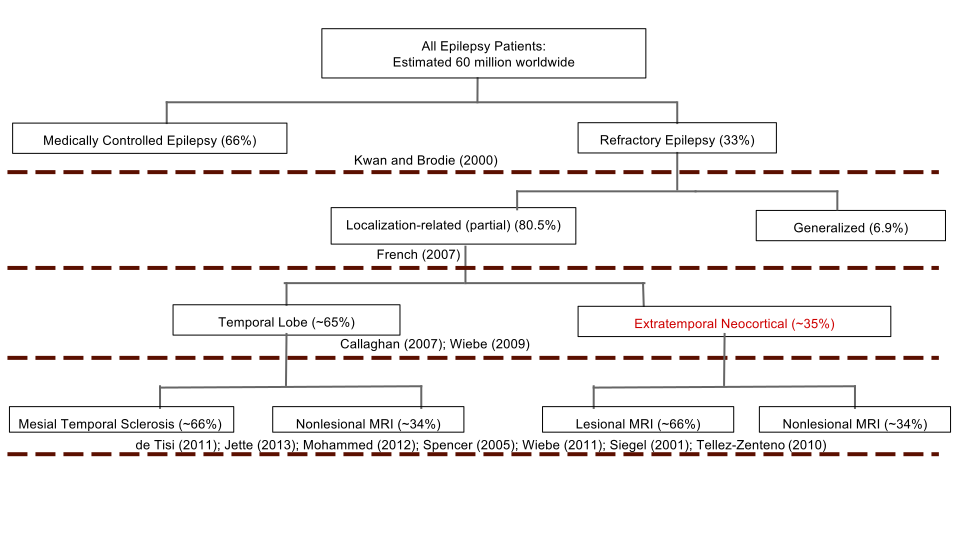
\includegraphics[width=\textwidth]{epilepsy_type}
\caption[Chart of epilepsy types]{\textbf{Population distribution of epilepsy types.} The distribution of patients with different types of epilepsies. The literature sources used to estimate population percentage is listed at each level. The focus of this work is extratemporal neocortical epilepsy, which has a prevalence of $\approx$6 million people.}
\label{epilepsy_type}
\end{figure}

\subsection{Clinical Imaging to Localize Structural and Functional Abnormalities}
While intracranial monitoring of neural activity associated with epileptic events is indispensable for identifying the seizure origin, multi-modal imaging can often identify lesions (\textbf{Fig.~\ref{typeIIfcd}}) (e.g. focal cortical dysplasia, tuberous sclerosis, other malformations of cortical development), which when resected lead to significantly better odds (2.9 times) of seizure freedom than in cases where imaging returns negative findings \cite{tellez-zenteno2010surgical}. For cases with unknown etiology, only $\approx$54\% of patients attain favorable seizure freedom (Engel score I or II) \cite{lee2005surgical}. Even in cases where no clear lesions are evident on MRI, clinicians collect a variety of imaging modalities providing orthogonal information about the epileptic network. We briefly introduce some of these imaging techniques below \cite{kuzniecky2002neuroimaging}:

\begin{figure}
\centering
\includegraphics[width=0.25\textwidth]{typeIIfcd_mri}
\caption[Example of brain lesion]{\textbf{Example of epileptogenic brain lesion.} A T2-weighted coronal FLAIR image displaying hyperintensity (white) in the inferior precuneus corresponding to a Type IIB focal cortical dysplasia, a common lesion underlying the development of focal seizures \cite{gaillard2015focal}.}
\label{typeIIfcd}
\end{figure}

\paragraph{Magnetic Resonance Imaging (MRI)}
T1 or T2-weighted imaging sequence that enables delineation of gray- and white-matter brain tissue. This imaging modality is most widely used for localizing aberrant migration of neural tissue associated with developmental disorders and investigating anatomical changes due to brain injury. Epilepsy cases with unremarkable MRI are colloquially considered \textit{non-lesional}.

\paragraph{Single Photon Emission Computed Tomography (SPECT)}
SPECT imaging is used in conjunction with an injectable radioactive tracer, which together yield a dynamic or static picture of blood perfusion through the brain. SPECT may be conducted during the ictal period to identify patterns of seizure onset and spread and, when compared to baseline interictal SPECT, can localize portions of the epileptic network in 70--90\% of patients \cite{kuzniecky2002neuroimaging}. The challenge for clinicians is accurate timing of conducting a SPECT study during seizures, which occur infrequently.

\paragraph{Positron Emission Tomography (PET)}
For epilepsy patients, PET is often used in conjunction with the radioactive tracer fluorodeoxyglucose (FDG), which together yield an estimate of metabolic activity in imaged tissue. While interictal PET has shown utility in localizing abnormalities in temporal lobe epilepsy, results are less promising for neocortical epilepsy. 

\subsection{Intracranial Monitoring of Brain Electrophysiology}
Although structural and functional imaging modalities provide significant information regarding abnormal brain tissue, the electrophysiology of neural circuits provide the clearest evidence of dysfunction when diagnosing epilepsy. A patient's neurological team will compile results from imaging and phase-I monitoring of scalp electroencephalography (EEG) and plan an invasive surgery to implant sub-dural, intracranial sensors for monitoring the electrocorticogram (ECoG) (\textbf{Fig.~\ref{intracranial_electrodes}}).  

\begin{figure}
\centering
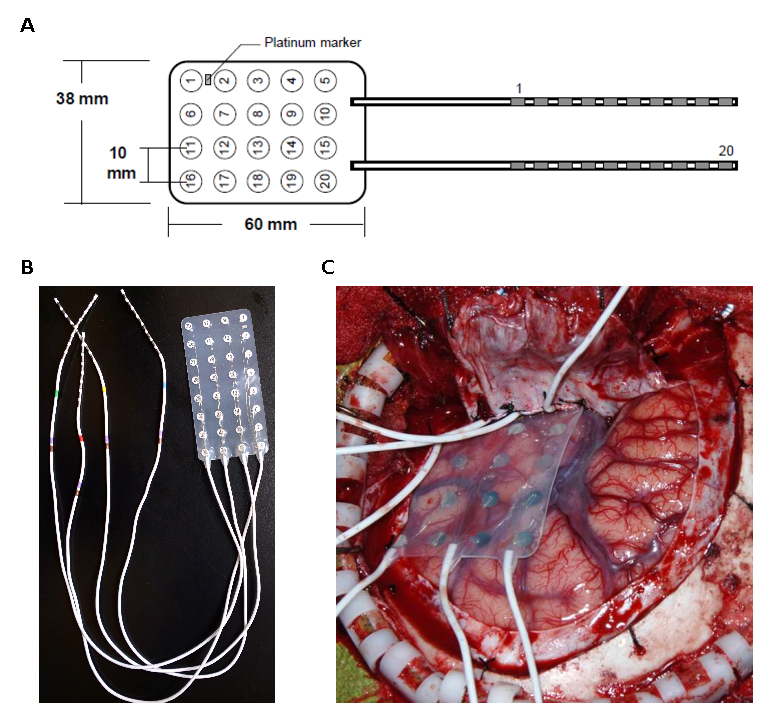
\includegraphics[width=\textwidth]{intracranial_electrodes}
\caption[Implantation of intracranial electrodes]{\textbf{Intracranial electrodes for monitoring epileptic cortex.} (\textbf{A}) Schematic of clinical-scale intracranial electrode with 20 sensors arranged in 4x5 configuration. Center-to-center distance between sensors is 10mm, and each sensor as a diameter of 4mm with 2.3mm exposed to the sub-dural cortical surface. (\textbf{B}) Photograph of a similar electrode with 32 sensors in 4x8 configuration. (\textbf{C}) Intraoperative photograph of implanted electrode in human epilepsy patient with reference to gyral, sulcal, and vascular anatomy.}
\label{intracranial_electrodes}
\end{figure}

Each sensor of an ECoG electrode is made from platinum-iridium and captures the local field potential (LFP) of neural activity from superficial layers of the neocortex \cite{buzsaki2012origin}. This LFP represents the extracellular voltage deflection from an aggregated population of neurons and is comprised of the population's synaptic activity and action potential firing patterns. Understanding the composition of the LFP is vital for connecting recorded ECoG activity to the behavior of underlying neural populations. While this is an active area of research, studies mostly agree that (i) action potentials generate a broad-band increase in the spectral power of the LFP, and (ii) spectral power in higher-frequency bands corresponds to more synchronous firing of action potentials, and (iii) higher-frequency components often phase-lock with lower-frequency components of the LFP, signifying a clear relationship between fluctuations of extracellular current and the action potentials produced by these currents \cite{buzsaki2012origin}. Below is list of frequency bands that are commonly identified in neural recordings of LFP and their physiological significance in terms of behavioral functioning:

\paragraph{Delta Band (0--4 Hz)}
Delta wave oscillations represent the slowest rhythms of LFP, and are typically recorded during the deepest stages of sleep (non-REM).

\paragraph{Theta Band (4--7 Hz)}
Theta wave oscillations are commonly observed in the hippocampus and the neocortex, although the putative functional role of this rhythm is different between the two brain regions. The hippocampal theta rhythm is typically found during behaviorally active states and have a purported relationship to learning and memory. The neocortical theta rhythm may have relevance to mechanisms of sleep and wakefulness.

\paragraph{Alpha Band (7--15 Hz)}
Alpha waves were the first discovered brain rhythm and have a strong relationship with activation of visual pathways and opening and closing of the eyes. 

\paragraph{Beta Band (15--30 Hz)}
Beta waves are believed to represent cognitive processes associated with consciousness. Additionally, beta rhythms are frequently recorded over motor cortex in conjunction with muscle contraction.

\paragraph{Low-Gamma Band (30--7 Hz)}

\paragraph{High-Gamma Band (4--7 Hz)} 













\begin{table}
\centering
\begin{tabular}{|c|ccc|r|}
	\hline
$k$ &  $x_1^k$    &   $x_2^k$  & $x_3^k$   & remarks  \\
	\hline
0   & -0.3 & 0.6 & 0.7  &  \\
1   & 0.47102965 & 0.04883157 & -0.53345964  & *\\
2   & 0.49988691 & 0.00228830 & -0.52246185 & $s_3$ \\
3   & 0.49999976 & 0.00005380 & -0.52365600  & \\
4   & 0.5 & 0.00000307 & -0.52359743  & $\epsilon < 10^{-5}$ \\
7   & 0.5 & 0 & -0.52359878  & $\epsilon < \xi $ \\
	\hline
\end{tabular}
\caption[A table of important values]{This is a table with {\emph very} important values!!!!!}
\label{important_values}
\end{table}
    
\uv plane
    $$ \pdfdx{f}{x} $$

\section{Blah} 
\lipsum
\begin{figure}
\centering
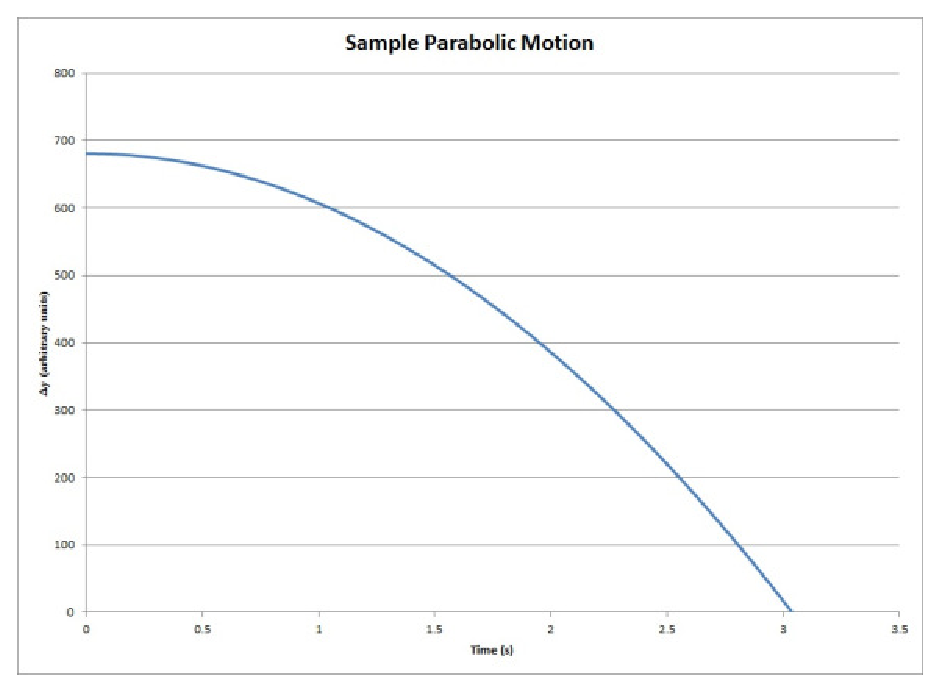
\includegraphics{parabolic_motion}
\caption[Parabolic Motion]{Here is parabolic motion as measured with science.}
\label{parabolic_motion}
\end{figure}
\lipsum

\chapter{Dynamic network drivers of seizure generation, propagation and termination}
\label{ch:netdrivers}

% the code below specifies where the figures are stored
\ifpdf
    \graphicspath{{chapters/ch3_figures/PNG/}{chapters/ch3_figures/PDF/}{chapters/ch3_figures/}}
\else
    \graphicspath{{chapters/ch3_figures/EPS/}{chapters/ch3_figures/}}
\fi


% ----------------------------------------------------------------------
%: ----------------------- content ----------------------- 
% ----------------------------------------------------------------------
\section{Abstract}
The epileptic network is characterized by pathologic, seizure-generating `foci' embedded in a web of structural and functional connections. Clinically, seizure foci are considered optimal targets for surgery. However, poor surgical outcome suggests a complex relationship between foci and the surrounding network that drives seizure dynamics. We developed a novel technique to objectively track seizure states from dynamic functional networks constructed from intracranial recordings. Each dynamical state captures unique patterns of network connections that indicate synchronized and desynchronized hubs of neural populations. Our approach suggests that seizures are generated when synchronous relationships near foci work in tandem with rapidly changing desynchronous relationships from the surrounding epileptic network. As seizures progress, topographical and geometrical changes in network connectivity strengthen and tighten synchronous connectivity near foci---a mechanism that may aid seizure termination. Collectively, our observations implicate distributed cortical structures in seizure generation, propagation and termination, and may have practical significance in determining which circuits to modulate with implantable devices.

\section{Introduction}
Localization-related epilepsy causes seizures that arise from one or more abnormal islands of cortical tissue in the neocortex or mesial temporal structures \cite{siegel2001medically}. In more severe cases, seizures with focal onset secondarily generalize, as pathologic activity spreads across the brain \cite{kutsy1999ictal}. Localization-related epilepsy represents $\approx$80\% of epilepsy cases and is often resistant to medication \cite{french2007refractory}. For drug-resistant patients, the only treatment options are implantable devices, or more traditionally resective surgery to remove enough cortical tissue in the epileptic network to decrease seizure frequency, while preserving brain tissue responsible for eloquent function. In surgical cases where discrete lesions associated with seizure onset (`foci') are not evident on an MRI, only $\approx$40\% remain seizure-free post-surgery \cite{french2007refractory}. The modest outcome associated with these procedures has lead investigators to further explore spatial distributions of epileptic activity using multiscale neural signals in ECoG and sub-millimeter $\mu$ECoG to more accurately localize where seizures start and how their pathologic activity spreads \cite{worrell2008high-frequency, schevon2009spatial, stead2010microseizures, viventi2011flexible, feldt_muldoon2013spatially, weiss2013ictal}. These approaches have spurred a paradigm shift from localizing just the foci towards informing interventions by mapping structural and functional connectivity of the whole epileptic network.

The notion of an epileptic network stems from the idea that pathologic functional connections and/or disconnections disrupt neural function, producing rhythmic motor activity, altered cognition, or abnormal sensation. Functional connections are time-dependent \cite{hutchison2013dynamic} communication pathways between neural populations that are measured by statistical relationships between electrode sensor (node) time series \cite{friston2011functional}, and that evolve according to brain state to produce behavior. The seizure state was originally considered to be hypersynchronous, or composed predominantly of strong functional connections. In contrast, a significant body of recent work presents compelling evidence that complex changes among strong (synchronized) and weak (desynchronized) network nodes accompany seizure dynamics \cite{wendling2003epileptic, jerger2005multivariate, schindler2006assessing, schindler2008evolving, kramer2010coalescence, jiruska2012synchronization}. The state-space of these dynamics are well described at the sensor level using measures of node centrality \cite{rummel2013systems-level, burns2014network}. However, epileptic network architecture at the basic sub-unit of individual connections is poorly understood, but tremendously powerful for discriminating fine-grain network changes that drive seizure dynamics.

Understanding the interplay between individual functional connections in the epileptic network is critical to answer questions goading clinical epileptologists and translational researchers: Where do seizures start? Can the epileptic network be modulated therapeutically? What can these methods reveal about the underlying neurophysiologic mechanisms? Progress in addressing these questions requires methods to track time-dependent functional connections within the epileptic network and understand their relative strengths and weaknesses, which in network terms are collectively referred to as the network's \emph{geometric} structure. Such methods would not only shed light on geographical dysfunction of epileptic foci, but also the disruption of normal brain tissue that is recruited during seizure events.

We hypothesize that the epileptic network achieves dysfunction and drives seizure activity by reconfiguring network connections during key network states that are clinically described as seizure generation, propagation, and termination. Our network reconfiguration hypothesis is informed by recent work demonstrating that human brain networks dynamically reorganize prior to changes in behavior \cite{bassett2011dynamic, ekman2012predicting}. During pathologic events, reconfiguration in epileptic networks may involve a redistribution of metabolic resources between strong and weak connections, supporting distinct network functions \cite{ercsey-ravasz2013predictive, santarnecchi2014efficiency}. Our results support this hypothesis, demonstrating that the epileptic network can be characterized by hubs of persistent strong connections surrounded by rapidly reconfiguring weak connections that drive seizure processes.

\section{Results}
To analyze the epileptic network, we retrieved ECoG recorded during simple partial, complex partial, and secondarily generalized seizures from 21 neocortical epilepsy patients undergoing routine pre-surgical evaluation of their epilepsy (see \textbf{Table~{\ref{ch3:tab1}}} for patient-specific information) through the \textit{International Epilepsy Electrophysiology Portal} (IEEG Portal, http://www.ieeg.org). We estimated weighted functional connectivity using a normalized cross-correlation metric (see \textit{Methods}) applied to non-overlapping, 1s time windows of ECoG (\textbf{Fig.~\ref{ch3:fig1}a}) This procedure results in a symmetric, $N \times N$ \textit{connectivity matrix} (specifying $\mfrac{N(N-1)}{2}$ unique connections in the upper or lower triangle of the symmetric connectivity matrix), where $N$ is the number of network nodes, for each of $T$ time windows analyzed. The pattern of unique network connections from a single time-window is a \textit{configuration vector}, which can be concatenated over all time windows to form a \textit{configuration matrix} of size $\mfrac{N(N-1)}{2} \times T$.

To better understand how global and local epileptic network geometry drive seizure dynamics, we study the configuration matrix during epileptic events divided into \textit{seizure} and \textit{pre-seizure} epochs (\textbf{Fig.~\ref{ch3:fig1}b}). 

\begin{table}
    \scriptsize
    \centering
    \begin{tabular}{|x{2cm}|x{0.5cm}|x{0.75cm}|x{2cm}|x{1.5cm}|x{1.25cm}|x{1cm}|x{1cm}|x{1.40cm}|}
        \hline
        Patient\newline (IEEG Portal) & Sex & Age (Years) & Seizure Onset & Etiology & Seizure Type & Seizures (N) & Imaging & Outcome \\ \hline \hline
        \verb|HUP64_phaseII| & M & 03/20 & Left frontal & Dysplasia & CP+GTC & 01 & L & ENGEL-I\\ \hline
        \verb|HUP65_phaseII| & M & 02/36 & Right temporal & Auditory reflex & CP+GTC & 03 & N/A & ENGEL-I\\ \hline
        \verb|HUP68_phaseII| & F & 15/26 & Right temporal & Meningitis & CP, CP+GTC & 05 & NL & ENGEL-I\\ \hline
        \verb|HUP70_phaseII| & M & 10/32 & Left perirolandic & Cryptogenic & SP & 08 & L & NR\\ \hline
        \verb|HUP72_phaseII| & F & 11/27 & Bilateral left & Mesial temporal sclerosis & CP+GTC & 01 & L & NR\\ \hline
        \verb|HUP73_phaseII| & M & 11/39 & Anterior right frontal & Meningitis & CP+GTC & 05 & NL & ENGEL-I\\ \hline
        \verb|HUP78_phaseII| & M & 00/54 & Anterior left temporal & Traumatic injury & CP & 05 & L & ENGEL-III\\ \hline
        \verb|HUP79_phaseII| & F & 11/39 & Occipital & Meningitis & CP & 01 & L & NR\\ \hline
        \verb|HUP86_phaseII| & F & 18/25 & Left temporal & Cryptogenic & CP+GTC & 02 & NL & ENGEL-II\\ \hline
        \verb|HUP87_phaseII| & M & 21/24 & Frontal & Meningitis & CP & 02 & L & ENGEL-I\\ \hline
        \verb|Study 004-2|   & F & 14/27 & Right temporal occipital & Unknown & CP+GTC & 01 & NL & ILAE-IV\\ \hline
        \verb|Study 006|     & M & 22/25 & Left frontal & Unknown & CP & 02 & NL & NR\\ \hline
        \verb|Study 010|     & F & 00/13 & Left frontal & Unknown & CP & 02 & L & NF\\ \hline
        \verb|Study 016|     & F & 05/36 & Right temporal orbitofrontal & Unknown & CP+GTC & 03 & NL & ILAE-IV\\ \hline
        \verb|Study 019|     & F & 31/33 & Left temporal & Unknown & CP+GTC & 15 & NL & ILAE-V\\ \hline
        \verb|Study 020|     & M & 05/10 & Right frontal & Unknown & CP+GTC & 04 & NL & ILAE-IV\\ \hline
        \verb|Study 023|     & M & 01/16 & Left occipital & Unknown & CP & 04 & L & ILAE-I\\ \hline
        \verb|Study 026|     & M & 09/09 & Left frontal & Unknown & CP & 10 & NL & ILAE-I\\ \hline
        \verb|Study 031|     & M & 05/05 & Right frontal & Unknown & CP+GTC & 05 & NL & NF\\ \hline
        \verb|Study 033|     & M & 00/03 & Left frontal & Unknown & GA & 07 & L & ILAE-V\\ \hline
        \verb|Study 037|     & F & 45/?? & Indeterminate & Unknown & CP & 02 & NL & NR\\ \hline
    \end{tabular}
    \caption[Patient data set for Chapter \ref{ch:netdrivers}]{\textbf{Patient information.} Patient data sets accessed through IEEG Portal (http://www.ieeg.org). Age (years) at first reported onset and at phase II monitoring. Localization of seizure onset and etiology is clinically-determined through medical history, imaging, and long-term invasive monitoring. Seizure types are SP (simple-partial), CP (complex-partial), CP+GTC (complex-partial with secondary generalization), or GA (generalized atonic). Counted seizures were recorded in the epilepsy monitoring unit. Clinical imaging analysis concludes L, Lesion; NL, non-lesion. Surgical outcome was based on either Engel score or ILAE score (scale: I-IV/V, seizure freedom to no improvement; NR, no-resection; NF, no follow-up). M, male; F, female. \label{ch3:tab1}}
\end{table}

\newpage
\begin{figure}[H]
    \centering
    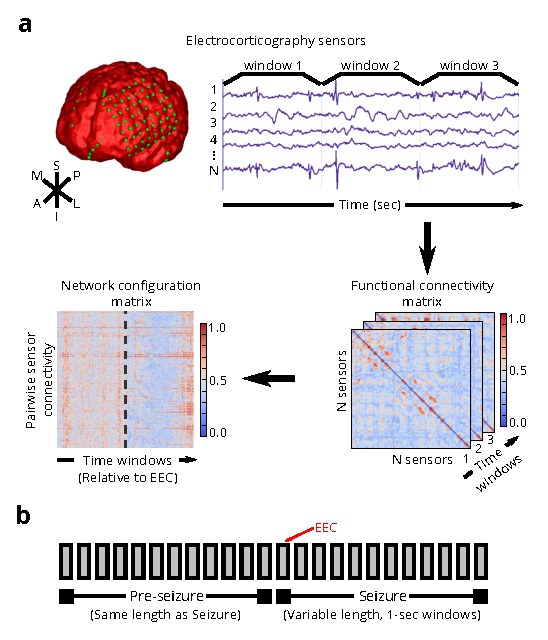
\includegraphics[width=0.5\textwidth]{panel1.eps}
\caption[Pipeline for measuring time-Varying functional networks]{\textbf{Analysis pipeline for dynamic epileptic networks.} (\textbf{a}) (\textit{Top}) We create functional networks based on electrophysiology by windowing ECoG signals collected from patients with drug-resistant neocortical epilepsy implanted with intracranial electrodes into 1s time windows. Each sensor is represented as a network node, and weighted functional connectivity between sensors, interpreted as degree of synchrony, is represented as a network connection. (\textit{Lower Right}) Functional connectivity is estimated by a magnitude normalized cross-correlation between sensor time series for each time window). (\textit{Lower Left}) We study temporal dynamics of each unique connection in a network configuration matrix. (\textbf{b}) For each epileptic event, we estimate dynamic functional connectivity during the seizure and the pre-seizure epoch. A seizure epoch consists of time windows between seizure onset -- as characterized by the earliest electrographic change (EEC) \cite{litt2001epileptic} -- and seizure termination. The associated pre-seizure epoch consists of an equal number of time windows as the seizure epoch and occurs immediately prior to the EEC. \label{ch3:fig1}}
\end{figure}


\subsection{Epileptic Network Reconfiguration Reveals Distinct Seizure States}
Do functional connectivity patterns significantly change as a seizure progresses? To answer this question, we developed a new method to uncover network states, defined by unique patterns of sensor-sensor functional connectivity between $T$ time windows (\textbf{Fig.~\ref{ch3:fig2}}). We define a \emph{network state} to be the set of all configuration vectors that exhibit a similar pattern of functional connectivity, more formally known in the network science literature as ``network geometry''. To quantify geometric similarity, we calculated the Pearson correlation coefficient between configuration vectors extracted from all possible pairs of $T$ time windows. This procedure produced a symmetric $T \times T$ configuration-similarity matrix (\textbf{Fig.~\ref{ch3:fig2}c}). 

We next ask whether clusters of time windows exhibit similar configuration patterns indicative of independent network states (\textbf{Fig.~\ref{ch3:fig2}d}). To test for distinct states in each epileptic event, we used an unsupervised clustering approach for networked data -- community detection -- that maximizes a modularity quality function $\mb{Q}$ obtained from the configuration-similarity matrix (see \textit{Materials}). In this approach, a structural resolution parameter $\gamma$ can be tuned to maximize the reliability of state estimates; we separately tuned this parameter for each seizure and pre-seizure epoch in each patient (See \textit{Supplemental Information}). This procedure assigns each time window to a community (or \emph{state}), and each state is composed of time windows that exhibit similar network geometry. Note that these time windows need not be temporally contiguous. We found that the epileptic network transitions through a variety of network states during pre-seizure and seizure epochs (\textbf{Fig.~\ref{ch3:fig3}a-b}). A comprehensive summary of epoch and state durations for each patient can be found in \textit{Supplemental Information: Table 1}. 

The existence of epileptic state transitions support the notion of a dynamically reconfiguring network. To quantify reconfigurability of the epileptic network, we measured the network \emph{flexibility}, or rate the of state change in each epoch (\textbf{Fig.~\ref{ch3:fig3}c}). We found that pre-seizure epochs display significantly higher flexibility ($\mu=0.665\pm0.205$) than seizure epochs ($\mu=0.274\pm0.165$) (paired-samples $t$-test; $t_{87}=-14.12$, $p=2.2\times10^{-16}$), indicating that the epileptic network transitions between states more slowly through seizure epochs than through pre-seizure epochs. Furthermore, pre-seizure epochs consisted of many short-duration states, while seizure epochs consisted primarily of 3 long states that occupy $\approx$87\% of seizure duration (\textbf{Fig.~\ref{ch3:fig3}d}). The three largest pre-seizure states occupied approximately 75\% of the epoch. Together, these results support the possibility that rapid changes in network geometry in pre-seizure epochs lead to seizures, and once there, the network undergoes slower geometric changes through 3 main dynamic states. To fairly assess differences in seizure and pre-seizure states, we retained the 3 longest network states from seizure ($S_0$, $S_1$, $S_2$) and pre-seizure epochs ($PS_0$, $PS_1$, $PS_2$) for the following analyses. 

\begin{figure}[H]
    \centering
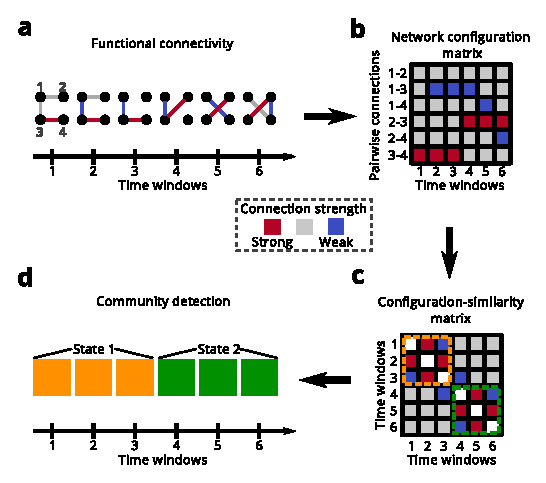
\includegraphics[width=0.5\textwidth]{panel2.eps}
\caption[Identifying discrete network states]{\textbf{Schematic for identifying network configuration states.} (\textbf{a}) We estimate dynamic functional connectivity; colors represent arbitrary connection strengths ranging from strong to weak (red, gray, blue). (\textbf{b}) We track all unique functional connections over time using a configuration matrix, in which each vector represents the set of connection weights for a 1s time window. (\textbf{c}) We compute the similarity between the network geometries of each pair of time windows using a Pearson correlation coefficient. In the resultant configuration-similarity matrix, colors represent the magnitude of similarity and visually identified clusters are distinguished by colored, dashed lines (orange and green). (\textbf{d}) We optimize a modularity quality function to cluster the configuration vectors (and thus time windows) into communities. Each cluster or community contains time windows with similar network geometry; colors represent assignments of time windows to different network configuration communities (orange and green). \label{ch3:fig2}}
\end{figure}

\begin{figure}[H]
    \centering
    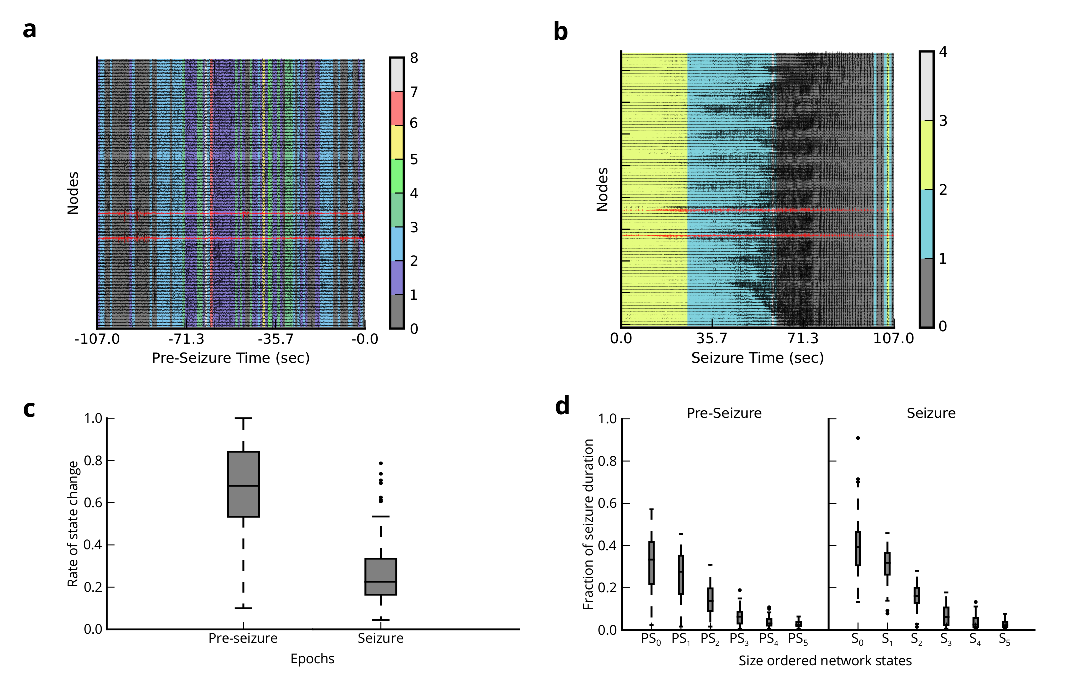
\includegraphics[width=\textwidth]{panel3.eps}
\caption[Discrete functional states of epileptic networks]{\textbf{Distinct dynamical states of epileptic networks.} (\textbf{a}) Example clustering of time windows to network states during a single pre-seizure epoch demonstrating rapid network reconfiguration. State assignments are overlaid on ECoG signals. Red traces correspond to seizure onset nodes. (\textbf{b}) Example clustering of time windows to network states during associated seizure epoch (from EEC to Termination) demonstrating slower network reconfiguration. (\textbf{c}) Network flexibility -- or average rate of network state transitions -- during pre-seizure and seizure epochs. The epileptic network displayed significantly more geometric reconfigurations during pre-seizure epochs than in seizure epochs ($N=88$, $p=2.2\times10^{-16}$). (\textbf{d}) Size-ordered distribution of total fractional duration of the 6 longest network states from each epoch (\textit{PS} (\textit{S}) indicates states of pre-seizure (seizure) epochs). All epochs are normalized to have duration of 1. We retain the first 3 network states of each epoch ($PS_0$, $PS_1$, $PS_2$, $S_0$, $S_1$, $S_2$) for the remaining analysis.} \label{ch3:fig3}
\end{figure}

\subsection{Epileptic Network Redistributes Connectivity During Seizures}
In the previous section, we observed that seizures progress through distinct states characterized by different functional connectivity patterns. To understand how these patterns differ, we used a two-pronged approach, examining (i) the strength of functional connections and (ii) the pattern of functional connections in different network states (\textbf{Fig.~\ref{ch3:fig4}a}). For simplicity, we report the strength of functional connections as a fraction of the total strength, and we refer to this quantity as the \emph{connection density}. Similarly, to characterize the pattern of functional connections, we examine the relative prevalence of synchronized (strong) versus desynchronized (weak) connections, and we refer to this quantity as the \emph{connection type index}.

The functional connection density measures the average connection strength in the network, where greater connection density indicates increased global network synchrony. We computed connection density by averaging the distribution of all connection strengths over all time windows in the given network state. We performed a one-way ANOVA to compare the effect of pre-seizure and seizure network states on connection density. We observed a significant effect of network state on connection density ($F_{5,474}=21.34$, $p<2\times10^{-16}$). Post-hoc analysis using Tukey's honest significant difference test (HSD) to control for a family-wise rejection error rate of 5\% (FWER=5\%) revealed a significant increase of connection density in each seizure state compared to any pre-seizure state. During the seizure, connection density increased between $S_0$ ($\mu=0.304\pm0.051$) and $S_1$ ($\mu=0.333\pm0.58$) ($p_{adj}=0.014$), and $S_0$ and $S_2$ ($\mu=0.338\pm0.052$) ($p_{adj}=0.002$), but did not significantly change between $S_1$ and $S_2$ ($p_{adj}=0.995$). Differences in connection density between the pre-seizure states ($PS_0$, $PS_1$, $PS_2$) were not significant. These results suggest synchronization increases as the network transitions from pre-seizure to seizure states. 

    While we observed an increase in global synchrony as seizures begin and progress, it is unclear whether this increase accompanies a change in functional connectivity pattern, and particularly in a switch from relative desynchronization (weak connectivity) to synchronization (strong connectivity). To type individual connections as strong or weak, we (1) compiled a distribution of all functional connections over all time windows across each event (encompassing the pre-seizure and seizure epoch), and (2) determined thresholds for connection type based on rank percentile, where \textit{strong} (\textit{weak}) connections were stronger (weaker) than 95\% of all connections. Based on connection type assignments in each epoch, we found the total number of strong ($C_s$) and weak ($C_w$) connections over all time windows in each network state and computed the connection type index as $\mfrac{C_s-C_w}{C_s+C_w}$. A strong type dominant network has a connection type index between $0$ and $+1$, where $+1$ implies all connections are strong, while a weak type dominant network has a connection type index between $0$ and $-1$, where $-1$ implies all connections are weak.

To determine the effect of network state on connection type index (\textbf{Fig.~{\ref{ch3:fig4}b}}), we conducted a one-way ANOVA test. We observed a significant effect of network state on connection type index ($F_{5,474}=70.41$, $p<2\times10^{-16}$). Post-hoc analysis using Tukey's HSD (FWER=5\%) indicated a significant change from weak type dominance during any pre-seizure state towards strong type dominance during seizure states. During the seizure, connection type index increased between $S_0$ ($\mu=0.023\pm0.498$) and $S_1$ ($\mu=0.437\pm0.417$) ($p_{adj}<2\times10^{-16}$), and $S_0$ and $S_2$ ($\mu=0.512\pm0.447$) ($p_{adj}<2\times10^{-16}$), but did not significantly change between $S_1$ and $S_2$. Differences of connection type index between the pre-seizure states ($PS_0$, $PS_1$, $PS_2$) ($\mu\approx-0.401$) were not significant.
    
Chronologically, the network is persistently desynchronized during the pre-seizure epoch, is driven to a quasi-synchronized seizure generation state $S_0$, and remains persistently synchronized as the seizure progresses through $S_1$ and $S_2$. A predominance of weak connections during a persistently desynchronized pre-seizure epoch coincides with earlier findings of improved network flexibility to reorganize during the same epoch. Unremarkable change in weak connection type dominance during the pre-seizure epoch suggests that the network simply redistributes weak connections amongst different nodes during this period. A critical transition to seizure generation during state $S_0$ is accompanied by synchronization towards more evenly distributed strong and weak connection types. As network flexibility decreases during the seizure, connections become more strong type dominant. To better understand how the network evolves through the desynchronized and synchronized states, we next study the impact of local, geographical changes in network geometry.

\begin{figure}[H]
    \centering
    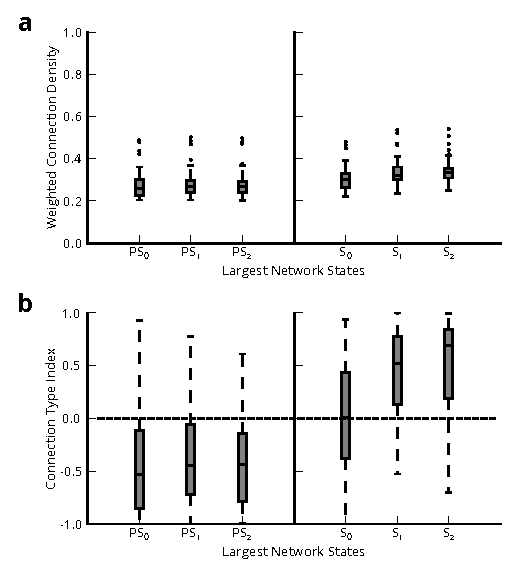
\includegraphics[width=0.5\textwidth]{panel4.eps}
    \caption[Global changes of connectivity in epileptic network states]{\textbf{Changes in global connectivity of epileptic networks}. (\textbf{a}) Functional connection density during pre-seizure ($PS$) and seizure ($S$) network states. We average connection strengths over all time windows within each network state ($N=80$). We found significant increase in connection density from all $PS$ to any $S$ network state, and significantly greater connection density during $S_2$ and $S_1$ compared to $S_0$. (\textbf{b}) Connection type index indicating strong or weak connection dominance during $PS$ and $S$ network states ($N=80$). We found significant change from weak type dominance during $PS$ to quasi weak-strong type dominance during $S_0$ and strong type dominance during $S_1$ and $S_2$.\label{ch3:fig4}}
\end{figure}

\subsection{Dynamic Regional Structure of the Epileptic Network}
In the preceding analyses, we demonstrated that the epileptic network displays weak type dominant connectivity during pre-seizure epochs and undergoes synchronizes to strong type dominance as the seizure initiates and progresses through 3 primary states. However, our approaches did not address whether these reconfigurations are spatially localized or distributed, and how they relate to seizure foci. To address these questions, we leveraged routine clinical procedures: A team of neurologists successfully identified the sensors on the seizure onset zone (SOZ) based on visual inspection of the intracranial recordings in 15 patients across a total of 50 seizures. We used this information to map connections in each seizure state to physical electrode locations in stereotaxic space (\textbf{Fig.~\ref{ch3:fig5}a}). 

To quantify spatial localization of connectivity relative to seizure foci and examine the role of network region in pre-seizure and seizure dynamics, we delineated the following three geographic types: (i) connections between nodes within the SOZ (SOZ-SOZ), (ii) connections between nodes outside the SOZ (OUT-OUT), and (iii) connections between one node within the SOZ and one node outside the SOZ (SOZ-OUT) (\textbf{Fig.~\ref{ch3:fig5}b}). We performed a two-way ANOVA test to compare the effects of geography and network state on connection strength. We observed a significant main effect of geography on connection strength ($F_{2,882}=158.501$, $p<2\times10^{-16}$) and a significant main effect of network state on connection strength ($F_{5,882}=26.394$, $p<2\times10^{-16}$). We also observed significant interactions between geography and network state ($F_{10,882}=2.871$, $p=0.002$). Post-hoc analysis on the interactions using Tukey's HSD (FWER=5\%) identified persistently stronger connection strength amongst SOZ-SOZ connections ($\mu\approx0.393\pm0.140$) relative to OUT-OUT ($\mu\approx0.282\pm0.059$) and SOZ-OUT ($\mu\approx0.284\pm0.059$) connections in every network state ($p_{adj}<1\times10^{-3}$). Connections in the SOZ-SOZ group were modestly strengthened during $S_0$ relative to $PS_0$ and $PS_2$ ($p_{adj}<0.05$), were greatly strengthened during $S_1$ and $S_2$ relative to any pre-seizure state ($p_{adj}<1\times10^{-3}$), and during the seizure only strengthened between $S_0$ to $S_2$ ($p_{adj}<0.05$). However, connection strengths in the SOZ-SOZ group did not significantly vary between pre-seizure states. Similarly, SOZ-OUT and OUT-OUT group did not significantly vary between any network states.

These results suggest that SOZ-SOZ connections are persistently the strongest of all network connection types during pre-seizure and seizure epochs. Upon seizure generation SOZ-SOZ connections strengthen incrementally, and then substantially as seizures progress. Nuancing our description of global network connectivity during pre-seizure and seizure epochs, which demonstrates a progression from desynchronization to synchronization over time, our results demonstrate that (i) desynchronization during pre-seizure states is primarily localized to SOZ-OUT and OUT-OUT connections, and (ii) resynchronization is primarily localized to SOZ-SOZ connections. Intuitively, desynchronous SOZ-OUT and OUT-OUT connections that frequently re-wire drives heightened network flexibility during pre-seizure epochs and synchronous SOZ-SOZ connections disrupts network flexibility during the seizure. 

To investigate the sensitivity and specificity of connection strength as a measure for identifying SOZ-SOZ connections, we employed receiver operating characteristic (ROC) analysis during pre-seizure and seizure epochs (\textbf{Fig.~\ref{ch3:fig5}c}). The ROC analysis evaluates the sensitivity and specificity of connections belonging to the SOZ-SOZ type as connection strength threshold is incrementally raised. We evaluate performance in detecting SOZ-SOZ connections by computing the area under the ROC curve (AUC) ranging from $0$ to $+1$, where values of $+1$ imply low sensitivity and false positives with high specificity and true positives. To assess significance of the AUC, we bootstrapped confidence intervals ($\alpha=0.05$) by re-assigning sensors to the SOZ uniformly at random without replacement 10000 times for each network state in both epochs. During seizure epochs, we found that $S_2$ was most effective at predicting SOZ-SOZ connections based on AUC ($\mu=0.849\pm0.169$) with significant AUC values in 32 of 50 seizures. Conversely $S_0$ was least effective at predicting SOZ-SOZ connections ($\mu=0.773\pm0.238$) with significant AUC values across 26 of 50 seizures. During pre-seizure epochs, SOZ-SOZ connections were similarly predictable across $PS_0$ ($\mu=0.709\pm0.268$) (significant in 25 of 50), $PS_1$ ($\mu=0.722\pm0.257$) (significant in 25 of 50), and $PS_2$ ($\mu=0.754\pm0.238$) (significant in 27 of 50). These results suggest that connection strength may be used to predict SOZ-SOZ connections during pre-seizure epochs with precision, but has better performance during more synchronized states such as $S_2$ compared to less synchronized states such as $S_0$.

\begin{figure}[H]
    \centering
    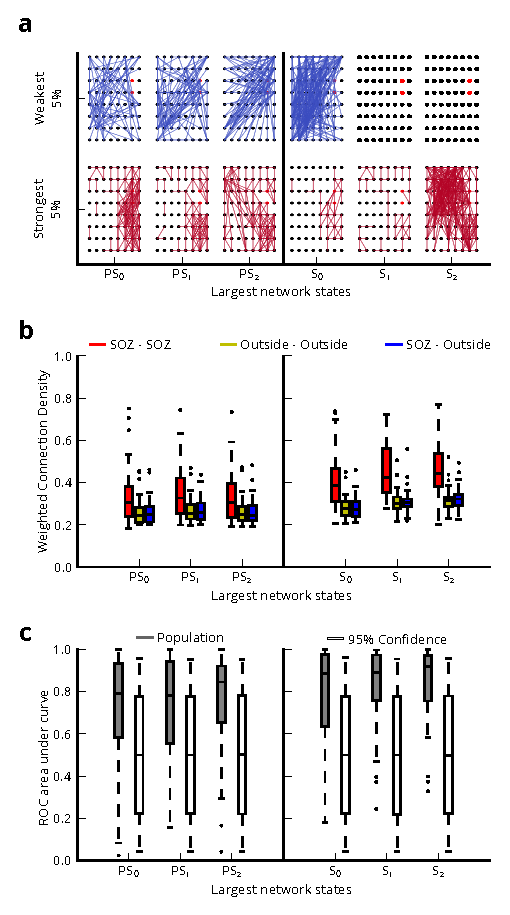
\includegraphics[height=0.75\textheight]{panel5.eps}
    \caption[Regional characteristics of epileptic network geography]{\textbf{Regional characteristics of network geography.} (\textbf{a}) Example of network geography with preserved 2-D spatial relationships between nodes for categories of strongest and weakest connections in upper and lower 5\% of connection strength distribution; Connection colors indicate weak (blue) and strong (red); the clinically-determined seizure onset sensors are shown in red. (\textbf{b}) Connection strength within 3 geographic connection types during $PS$ and $S$ network states ($N=50$). During $PS$ and $S$, we observed significantly stronger connections amongst SOZ-SOZ regions than OUT-OUT and SOZ-OUT regions. During $S$, we observed significant increase in SOZ-SOZ connections as seizures initiate and progress. (\textbf{c}) ROC AUC compared to 95\% bootstrapped confidence intervals using connection strength to predict SOZ-SOZ connections during $PS$ and $S$ network states ($N=50$). The synchronized $S_2$ state yielded the best performance, while the desynchronized $PS_0$ state yielded the worst performance. \label{ch3:fig5}}
\end{figure}

\subsection{Impact of Surrounding Connectivity on Epileptic Network Dynamics}
Thus far we have seen how connectivity associated with the SOZ synchronizes the epileptic network during seizures. However, it is unclear whether involvement from the broader epileptic network aids or disrupts pre-seizure and seizure dynamics. 

We first hypothesized that changes in network geometry are not limited to redistribution of connection strengths, but may also involve topographical changes in connection lengths accompanying changes in functional network anatomy. In a sample of pre-seizure and seizure states, we observed clustering of strong connections while weak connections distributed more broadly (\textbf{Fig.~{\ref{ch3:fig5}a}}). To test our hypothesis, we restricted our analysis to connections within electrode grids with uniformly spaced nodes in $8 \times 8$, $8 \times 6$, $6 \times 6$, or $4 \times 6$ configurations (in 75 seizures over 19 patients) and computed average Spearman's rank correlation coefficient between connection length and connection strength over all time windows of each network state (\textbf{Fig.~{\ref{ch3:fig6}a}}). A more positive (negative) correlation coefficient indicated stronger connections were longer (shorter). A one-way ANOVA test was conducted to compare the effect of pre-seizure and seizure network states on correlation between connection length and connection strength. We observed a significant effect of network state on correlation ($F_{5,444}=9.348$,  $p=1.76\times10^{-8}$). Post-hoc analysis using Tukey's honest significant difference test (HSD) to control for a family-wise rejection error rate of 5\% (FWER=5\%) revealed significant increase in negative correlation between connection length and strength in $S_0$ ($\mu=-0.225\pm0.92$) compared to $PS_2$ ($\mu=-0.182\pm0.091$) ($p_{adj}<0.05$) but not $PS_0$ ($\mu=-0.188\pm0.100$) or $PS_1$ ($\mu=-0.189\pm0.092$). Connection length is significantly more negatively correlated with connection strength in $S_1$ ($\mu=-0.258\pm0.081$) and $S_2$ ($\mu=-0.242\pm0.086$) compared to any pre-seizure state ($p_{adj}<0.01$). There was no significant change in correlation between pre-seizure states or seizure states.
    
In summary, we found that stronger connection strengths are present in connections with shorter lengths, regardless of network state. During seizures, reorganization in the epileptic network leads to further lengthening of weaker connections and shortening of stronger connections. Coinciding with the earlier finding that seizure generation involves quasi-synchronization of the network, we find a modest shortening of strong connections relative to the pre-seizure period. As seizures progress, synchronous connections tighten to more local regions, while desynchronous connections stretch further into the broader epileptic network.

\begin{figure}[H]
    \centering
    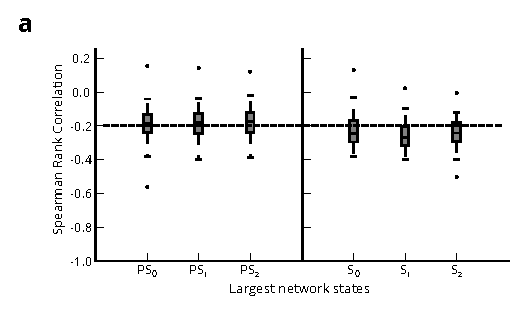
\includegraphics[width=0.5\textwidth]{panel6.eps}
\caption[Topographical characteristics of epileptic network connectivity]{\textbf{Topographical characteristics of network connectivity.} (\textbf{a}) Average Spearman's rank correlation coefficient between connection length and strength in $PS$ and $S$ epochs ($N=75$). Physical connection lengths computed from regularly spaced nodes in electrode grid; connection lengths measured in millimeters. Stronger connections are consistently shorter than weaker connections. During $S$, there is significant topographical reorganization making weak connections longer and strong connections tighter. \label{ch3:fig6}}
\end{figure}


\section{Discussion}
\subsection{Epileptic Network Reconfiguration}
Intuitively, complex reconfiguration of functional brain networks can accompany changes in cognitive state or changes in behavior. Prior fMRI studies have explored such reconfiguration in whole-brain networks constructed from data acquired during motor skill learning \cite{bassett2011dynamic} and as task states change \cite{bassett2006adaptive}, and in networks impacted by stroke \cite{wang2010dynamic, grefkes2011reorganization}. In contrast, here we explore the reconfiguration of a local area and use higher resolution ECoG data to map the fine-scale temporal dynamics of reconfiguration processes.

In this study, we developed and exercised a novel method for distinguishing brain states based on differences in time-dependent functional network geometry. Our approach expands upon previous notions of state-space in dynamic epileptic networks \cite{rummel2013systems-level, burns2014network}, by tracking changes between node pairs (connections) rather than in node importance (centrality). An important advantage associated with this technique is that network reorganization can be studied without \emph{a priori} knowledge of specific topological structure, such as small-worldness \cite{kramer2010coalescence}. Rather, time-dependent changes in connectivity are based simply on similarities in signal statistics.

We applied our technique to a set of human ECoG recordings, and extracted network dynamics during seizure and pre-seizure epochs. We found that seizures exhibit at least three network states ($S_0$, $S_1$, $S_2$) and that the epileptic network progresses through these states more slowly in comparison to the period preceding seizure generation. Our results are in line with prior work that has shown more frequent state changes during the interictal period in comparison to seizures \cite{burns2014network}. Next, we provide a mechanistic explanation of how state changes operate with strong and weak regimes of connectivity to drive seizures through neurologically-defined onset, propagation and termination states ubiquitous in clinical descriptions.

\subsection{Balance of Strong and Weak Connections}
Our analytical approach utilizes the distribution of functional connection strengths to characterize connections as ``strong'' (synchronous) or ``weak'' (desynchronous), rather than simply stating that two sensors are functionally ``connected'' or ``not connected''. Mathematically, this focus corresponds to a study of network \emph{geometry} as opposed to network \emph{topology}. A primary advantage of the weighted network approach is the ability to separate connections into classes that differ in strength. Evidence suggests that strong and weak connections play different roles in supporting cognitive function \cite{schneidman2006weak, santarnecchi2014efficiency}. Traditional thought is that strong connections represent primary communication pathways between brain areas. However, recent work demonstrates that weak connections support increased network efficiency and may play a large role in distinguishing pathologic \cite{bassett2012altered} and healthy \cite{cole2012global, santarnecchi2014efficiency} network states. From a dynamical perspective, strong connections may persistently engage throughout neurophysiological processes, whereas weak connections may engage transiently to enable brain state transitions.

Prior work has speculated that the epileptic network is connected at the beginning of the seizure, disconnected in the middle, and finally reconnected at the end \cite{wendling2003epileptic, schindler2006assessing, kramer2010coalescence}. However, our results suggest that a more accurate way to address this hypothesis is to consider the strength of functional connections and disambiguate slower temporal dynamics occurring at each node, independently, which may elevate spurious connectivity between disconnected regions. 

Using a weighted connectivity approach, we find that connections in the epileptic network have more weak than strong connections during $PS_0$, $PS_1$, and $PS_2$, states preceding the electrographic seizure onset, a near balance of strong and weak connections during $S_0$, which corresponds to seizure generation, and more strong than weak connections during $S_1$ and $S_2$ states representing seizure progression and termination. It is possible that clinician subjectivity in marking the time of seizure onset may explain our result of disconnectivity before seizure generation, which contrasts with prior reports of a disconnected network at either seizure onset or mid-seizure \protect{\cite{wendling2003epileptic, schindler2006assessing, kramer2010coalescence}}. Our method places greater emphasis on connectivity derived from faster activity by reducing contribution from slower dynamics (see \textit{Methods}) and corroborates clinical belief that seizure generation during $S_0$ involves a gradual transition from desynchronous to synchronous connectivity, which peaks during the termination phase of the seizure ($S_2$). 

Mechanistically, the weak connectivity that we observe preceding seizure generation benefits from high network flexibility to drive seizure generation through a rapid reorganization of weaker connections in the epileptic network. As seizures initiate and progress, the epileptic network redistributes weak connectivity to strong connectivity while network flexibility is concurrently diminished. In relation to prior work that demonstrates a propensity for the epileptic network to follow a recurring pattern of state transitions during seizures \cite{burns2014network}, our results suggest that weak connectivity preceding the seizure drives the network to a more predictable series of increasingly synchronized states during seizures. Next, we explore beyond global network structure and discuss how regional connectivity dynamics provide further insight on network drivers of seizure evolution.

\subsection{Regional Connectivity Regulates Seizure Evolution Dynamics}
While temporal network structure provides rich information regarding seizure states, it does not directly provide information regarding the spatial processes involved in seizure dynamics. We therefore complemented the temporal network approach by incorporating information about sensor role either within or outside the seizure onset zone and sensor location in Euclidean space. Our results demonstrate that these additional spatial features provide new insights into potential neurophysiological mechanisms involved in seizure generation, and may inform the development of clinical tools for objectively isolating the seizure onset zone directly from seizure or pre-seizure data.

Prior work has demonstrated high synchronization within the seizure onset zone during interictal epochs \cite{dauwels2009localization, warren2010synchrony}. However, the temporal dynamics and geometrical roles of these two sets of areas has remained elusive. Our results elucidate the role played by seizure onset regions during seizures and the accompanying recruitment of the surrounding epileptic network during termination. Clear isolation of the seizure onset zone exists in pre-seizure periods, suggesting the potential to identify foci, niduses of seizure generation, within the network from inter-ictal data. Critically, connectivity within the onset zone strengthens during early seizure periods ($S_1$) and intensifies as seizures progress ($S_2$) and terminate ($S_3$), suggesting that the onset zone drives the transition from global desynchronization to synchronization during seizure generation and persists in this functional role through the entire seizure. Such a mechanism also points to a role of the onset zone in seizure termination, potentially in tandem with topographical mechanisms, which we discuss in the next section.


\subsection{Network Tightening During Seizures}
Our observation that stronger connections are typically short and weaker connections are typically long, is consistent with results from two lines of research: (i) functional studies in healthy individuals that utilize other imaging modalities such as fMRI \cite{santarnecchi2014efficiency} and (ii) structural connectivity studies in non-human primates that utilize tract tracing techniques \cite{ercsey-ravasz2013predictive}. In epilepsy, prior work has shown hubs of connectivity proximal to the seizure onset zone \cite{schevon2007cortical, zaveri2009localization-related, rummel2013systems-level}, however their role in seizure dynamics was previously unknown. We show that seizure generation leads to further shortening of stronger connections and lengthening of weaker connections, suggesting that stronger connections are physically tightening, perhaps into more functionally cohesive portions of cortex during seizures. We speculate that the tightening of stronger connections to localized sub-networks might act as a control mechanism to quench disruptive network activity that may have built-up over many hours prior to the seizure through increasing frequency of epileptiform discharges \cite{litt2001epileptic} or facilitate previously described compensatory mechanisms \cite{rummel2013systems-level}. Conversely, weaker connections are longer during seizure periods than pre-seizure periods and could be a vehicle for spreading desynchronous activity broadly.

\subsection{Clinical Impact and Future Work}
We have seen that the dynamical processes that propel epileptogenic networks into seizures can be complex and are poorly understood. Yet, clinicians rely on visual inspection to describe spatial and temporal properties of seizures. The lack of standardized clinical measures to mark epileptic events calls for the development of automated methods. The network analysis tools we have built, while generally applicable to any dynamic network, can parse seizure states, localize driver `foci' of seizures, and characterize how seizures progress and terminate. This interpretation can be translated into useful clinical tools to identify dysfunctional anatomical regions that drive the epileptic network and may be particularly amenable to local interventions, such as surgery or device placement. Of interest, seizure driving `foci' were equally present in the half of our study patients who did not have focal lesions on brain imaging, compared to those patients with lesions demonstrated on MRI. We plan a more detailed study in the future to correlate mapping of these seizure-driving regions with brain resection and outcome. 

Currently, our tools employ community detection techniques to identify gross changes in the meso-scale architecture of network structure across time. The observed meso-scale reconfiguration processes may be accompanied by region-specific trends in reconfiguration between the epileptic network and surrounding healthy networks. A remaining gap is understanding how functional dynamics map to structural features of the epileptic network using fiber-tracking techniques to describe how seizures start and then spread through white-matter. Additionally, this work could be used to address cellular mechanisms by considering micro-scale reconfigurations. Recent studies suggest that epileptic networks in the neocortex may be composed of distributed micro-domains on the scale of a few cortical columns generating high frequency oscillations and micro-seizures that coalesce in a network during seizure generation and termination \cite{stead2010microseizures}. While of great interest, these studies are currently limited by the lack of appropriate implantable high-resolution sensors capable of covering clinically relevant areas sufficiently to yield comprehensive high-resolution maps. Further development of dynamic community detection methods to identify and track reconfiguration within network sub-regions at both the meso and micro-scales may help delineate healthy and pathologic networks and uncover mechanisms of network recruitment.

An important clinical consideration related to this work is the impact of sampling error inherent in any intracranial implantation procedure on our results. Any technique used to map epileptic networks, subdural electrode strips and grids, more distributed ``Stereo EEG'' implantations, and combinations of these two approaches, usually yield incomplete representations of epileptic networks. It is not possible to fully record from the entirety of cortex in affected patients. In some cases this might mean that neither seizure onset zones nor all regions of seizure spread are fully delineated.  Despite this incomplete representation, the presence of three clear states defining seizures in each of the patients presented above, and their objective and independently determined relationship to the seizure onset zone suggest that our findings are important and real. With further validation on a larger number of patients with both lesional and non-lesional epilepsies, we hope to demonstrate the utility of our method to define functional components of epileptic networks. Our method shows promise for informing epilepsy surgery and for placing devices into regions that drive seizure generation and termination. Future work will focus on using these methods to compare competing approaches for localizing epileptic networks, such as subdural and stereo EEG.  It is intuitively plausible that each will have advantages in recording components of epileptic networks in different types of localization-related epilepsy.

\section{Materials and Methods}
\subsection{Ethics Statement}
    All patients included in this study gave written informed consent in accord with the University of Pennsylvania Institutional Review Board and Mayo Clinic Institutional Review Board for inclusion in this study.

\subsection{Patient Data Sets}
Twenty-one patients undergoing surgical treatment for medically refractory epilepsy believed to be of neocortical origin underwent implantation of subdural electrodes to localize the seizure onset zone after noninvasive monitoring was indeterminate. De-identified patient data was retrieved from the online International Epilepsy Electrophysiology Portal (IEEG Portal) \cite{wagenaar2013multimodal}. ECoG signals were recorded and digitized at either 512 Hz (Hospital of the University of Pennsylvania, Philadelphia, PA) or 500 Hz (Mayo Clinic, Rochester, MN) sampling rate. Surface electrode (Ad Tech Medical Instruments, Racine, WI) configurations, determined by a multidisciplinary team of neurologists and neurosurgeons, consisted of linear and two-dimensional arrays (2.3 mm diameter with 10 mm inter-contact spacing) and sampled the neocortex for epileptic foci (depth electrodes were first verified as being outside the seizure onset zone and subsequently discarded from this analysis). Signals were recorded using a referential montage with the reference electrode, chosen by the clinical team, distant to the site of seizure onset and spanned the duration of a patient's stay in the epilepsy monitoring unit.

\subsection{Description of Seizure Events}
We analyzed a total of 88 seizure events, including simple partial, complex partial, and secondarily generalized, stemming from neocortical foci in this study. Seizure onset time and localization were defined by the point of earliest electrographic change (EEC) and annotated and marked by a team of practicing epileptologists \cite{litt2001epileptic}. ECoG signal directly preceding each seizure and equal in duration to that seizure was also extracted for balanced comparison and labeled as pre-seizure.

\subsection{Extracting Dynamic Functional Networks}
Signals from each epoch were divided into $1$-second, non-overlapping, wide-sense stationary time windows in accord with other studies \cite{kramer2010coalescence} and subsequently pre-processed. To test the biasing effect of high-amplitude spiking on signal connectivity measurements, we also investigated windows $0.5$-seconds in duration to sample more of the non-biasing temporal space and found similar results. In each time window, signals were re-referenced to the common average reference \cite{kramer2010coalescence, towle1999electrocorticographic} to account for variation in reference location across patients and to avoid broad field effects that may bias connectivity measurements erroneously in the positive direction. Each window was filtered at 60 Hz to remove line-noise, and low-pass and high-pass filtered at 120 Hz and 1 Hz, respectively, to account for noise and drift. To limit sources of volume conduction from introducing spurious connectivity, we pre-whiten signals in each window using a first-order autoregressive model to account for slow dynamics. This accomplishes two goals: (i) flattening of the signal power spectrum to enhance higher-frequency content that contains local neural population dynamics that is less affected by volume conduction, and (ii) decreases the influence of independent node dynamics when computing correlation-based connectivity measurements \cite{towle1999electrocorticographic, bullmore2001colored, lund2006non-white, arbabshirani2014impact}.

Dynamic functional networks were formed by applying a normalized cross-correlation similarity function $\bs{\rho}$ between the time series of two sensors in the same time window using the formula
    \begin{eqnarray}
        \bs{\rho}_{\mb{xy}}(\mb{k}) = \underset{\tau}{\operatorname{argmax}}\:{\mathrm{E}}[(\mb{x_k}(t) - \mu_{\mb{x_k}})(\mb{y_k}(t+\tau) - \mu_{\mb{y_k}})]
    \end{eqnarray}
    where $\mb{x}$ and $\mb{y}$ are signals from one of $\mb{N}$ sensors or network nodes, $\mb{k}$ is one of $\mb{T}$ non-overlapping, one-second time windows, and $\mb{x_{k}}=\mb{y_{k}}=0$. The $\mb{N}$x$\mb{N}$x$\mb{T}$ similarity matrix is also known as a network adjacency matrix $\mb{A}$ (\textbf{Fig.~\ref{ch3:fig1}a}). In our weighted network analysis approach, we retain and analyze all possible connection weights between nodes.

\subsection{Computing Network States}
    Network states, or temporal changes in network geometry, was tracked separately in each epoch by clustering the configuration-similarity matrix through a community detection technique known as modularity optimization. We construct the configuration-similarity matrix by first unraveling $\mb{A}$ to a network evolution matrix $\mb{\hat A}$ describing the weights of $\mfrac{\mb{N}(\mb{N}-1)}{2}$ connections across $\mb{T}$ time windows. Using a Pearson correlation coefficient to measure similarity, we transform $\mb{\hat A}$ to a fully-connected $\mb{T}$x$\mb{T}$ configuration state adjacency matrix $\mb{S}$. The configuration adjacency matrix is partitioned into communities by maximizing the modularity index $\mb{Q}$ \cite{newman2004finding} using a Louvain-like locally greedy algorithm \cite{blondel2008fast}. We employed a Newman-Girvan null model \cite{newman2006modularity, porter2009communities} and adaptively determined an optimal structural resolution parameter $\gamma$ per seizure (see \textit{Supplemental Information}; and \cite{bassett2013robust} for a more detailed discussion of resolution parameters in modularity maximization). We used a consensus partition method with 1000 optimizations per run until we obtained consistent community partitioning \cite{lancichinetti2012consensus, bassett2013robust}. The three longest communities (clusters, or network states) from each seizure were selected for further analysis and re-labeled in order of median temporal occurrence for population-level comparison.

\subsection{Distinguishing Connection Types}
    Connections were classified as \emph{strong} or \emph{weak} based on thresholds determined by the distribution of connection strengths for each epoch separately for each seizure. The strong (weak) connections must be $>$95\% ($<$5\%) of all connection strengths. To measure the dominance of \emph{strong} or \emph{weak} connections, we defined the connection type index as
    \begin{eqnarray}
        \mb{B} = \frac{\mb{C_s}-\mb{C_w}}{\mb{C_s}+\mb{C_w}}
    \end{eqnarray}
where $\mb{C_s}$ and $\mb{C_w}$ are the average number of strong and weak connections over possible connections and number of time windows.

\subsection{Measuring Network Topography}
Connection topography metrics were computed for only within-grid electrodes, ignoring all other non-grid electrodes such that inter-electrode spacing in all analyses was kept constant. We related connection strength to the two-dimensional physical distance between nodes (electrode sensors) of that connection in millimeters.

\section{Acknowledgments}
    AK and BL acknowledge support from the National Institutes of Health through awards \#R01-NS063039, \#1U24 NS 63930-01A1, the Citizens United for Research in Epilepsy (CURE) through Julie's Hope Award, and the Mirowski Foundation. DSB acknowledges support from the John D. and Catherine T. MacArthur Foundation, the Alfred P. Sloan Foundation, the Army Research Laboratory, the Institute for Translational Medicine and Therapeautics, the National Institute of Mental Health through award number 2-R01-DC-009209-11 (Thompson-Schill), and the National Science Foundation awards CRCNS BCS-1441502 and BCS-1430087 through the ENG, CISE, and SBE directorates. The content is solely the responsibility of the authors and does not necessarily represent the official views of any of the funding agencies. We thank Sarah F. Muldoon, Urs Braun, Shi Gu, Qawi Telesford, Lohith Kini, Hoameng Ung for comments on earlier versions of this manuscript.

\section{Supplemental Information}
\subsection{Network States}
For dynamic networks there is a lack of approaches to quantify how the pattern of connections between nodes, or the gross network configuration, varies over time. Clusters of time windows in which network configurations look similar can be thought as network states. In networks where $N$ nodes stay constant over all $T$ time windows, we can describe the state of $\frac{N(N-1)}{2}$ possible connections between all nodes in each time window $t=1~\mathrm{to}~T$ by a \textit{configuration vector} $\vec{v_{t}} \in \mathbb{R}^{\frac{N(N-1)}{2}}$; collectively forming a \textit{configuration matrix} $\textbf{V} \in \mathbb{R}^{\frac{N(N-1)}{2}\times T}$. Intuitively, changes in $\vec{v_{t}}$ between different $t$ can imply dynamical changes in network connectivity.

While dynamic networks commonly experience meso-scale changes in connectivity over time, there is currently no way to determine whether these meso-scale changes contribute to gross reconfiguration of the entire network. Using a similarity function (herein we use Pearson correlation coefficient), we quantify the degree of change in connectivity patterns in $\textbf{V}$ between all $T$ time windows stored in a symmetric \textit{configuration-similarity matrix} $S \in \mathbb{R}^{T\times T}$. In this work we are interested in clustering time windows that express similar network configuration patterns. To this end, we employ static community detection techniques to group time windows with similar gross network configuration.


\section{Modularity optimization for community detection}
\subsection{Theory}
Community detection is a technique often used to study meaningful group structure in complex networks by clustering nodes into `modules' or `communities'. A community can be thought of as a set of nodes that are connected among one another more densely than they are to nodes in other communities. A popular way to identify community structure is to optimize a quality function known as modularity $\mb{Q}$, which has been shown to extract meaningful functional components of networks by comparing the real network to a null model \cite{newman2004finding, newman2006modularity, porter2009communities, fortunato2010community}. While these approaches have been mainly applied to both binarized and weighted static networks, more recent extensions of the model investigate dynamic communities that group nodes over time. In our work we apply static community detection to the configuration-similarity matrix, viewed as a fully connected graph where each node represents the similarity of the configuration vector $\vec{v_{t}}$ between time windows $t_1$ and $t_2$ where $t_1=t_2=0$, to group gross network configuration patterns into communities.  

In general, to perform community detection one begins with a network of $N$ nodes and a given set of connections between those nodes. A static network is then represented using an $N \times N$ adjacency matrix $\mathbf{A}$. The element $A_{ij}$ of the adjacency matrix represents a connection from node $i$ to node $j$ where $i=j=0$, and its value indicates the weight of that connection. Then, $\mb{Q}$ is formally defined as:
\begin{equation}\label{modopt}
	Q = \sum_{ij} [A_{ij} - \gamma P_{ij}] \delta(g_{i},g_{j})\,,
\end{equation}
where node $i$ is assigned to community $g_{i}$, node $j$ is assigned to community $g_{j}$, the Kronecker delta $\delta(g_{i},g_{j})=1$ if $g_{i} = g_{j}$ and it equals $0$ otherwise, $\gamma$ is the \emph{structural resolution parameter}, and $P_{ij}$ is the expected weight of the edge connecting node $i$ to node $j$ under a specified null model. The choice $\gamma = 1$ is very common, but it is important to consider multiple values of $\gamma$ to examine groups at multiple scales (see \textit{SI Section \ref{subsec:structres}}). A commonly chosen null model is the Newman-Girvan null model \cite{porter2009communities, fortunato2010community, newman2004finding, newman2006modularity} defined as:
\begin{equation}\label{newgirv}
    P_{ij} = \frac{k_i k_j}{2m}
\end{equation}
where $k_i=\sum_j A_{ij}$ is the strength of node $i$ and $m=\frac{1}{2}\sum_{ij}A_{ij}$ is the average strength over all connections. 

Maximizing $Q$ partitions the network into communities such that the total within-community connection weight is maximum relative to the null.

\subsection{Structural resolution parameter for community detection}
\label{subsec:structres}
The structural resolution parameter $\gamma$ of the modularity quality function can be used to identify community structure over different topological or geometric scales \cite{reichardt2006statistical, fortunato2007resolution, porter2009communities, mucha2010community, bassett2013robust}. Typically, $\gamma$ is chosen to be equal to 1. However, by varying $\gamma$, one can examine fine grain structure in networks by extracting smaller communities. In our application, we were interested in determining community structure of configuration-similarity matrices with a variable (i) number of sensors implanted per patient, (ii) seizure duration and (iii) spatial extent of epileptogenic cortex. Each of these factors can potentially impact the scale at which appreciable meso-scale functional reorganization can be detected.

Prior studies have explored a structural resolution parameter limit that represents a trade-off between grouping all nodes into a single community with large modularity (low $\gamma$) and grouping each node into separate communities with low modularity (high $\gamma$) \cite{fortunato2007resolution}. In real-networks \cite{bassett2013robust} modularity and structural resolution share an approximate inverse power relationship, suggesting an optimal $\gamma$ may occur as rate of change in modularity decreases (within increasing $\gamma$). Such a phenomenon would occur at the inflection point for change in modularity as the $\gamma$ parameter is tuned.

To determine an optimal $\gamma$ parameter for each configuration-similarity matrix (per epoch, per patient), we computed the inflection point in modularity $\mb{Q}$ at each $\gamma$ between $0.8$ and $1.3$ in intervals of $0.01$ (\textbf{Fig.~S\ref{ch3:figS1}}). We define the optimal $\gamma$ to be the $\gamma$ at which the inflection point occurs. The optimal $\gamma$ (\textbf{Fig.~S\ref{ch3:figS2}}) was significantly different between the pre-seizure epochs and seizure epochs, based on $t$-test ($t_{87}=2.64$, $p<0.01$). This result demonstrates that the granularity of network state division is significantly greater during seizure epochs than pre-seizure epochs.

\begin{figure}[H]
    \centering
    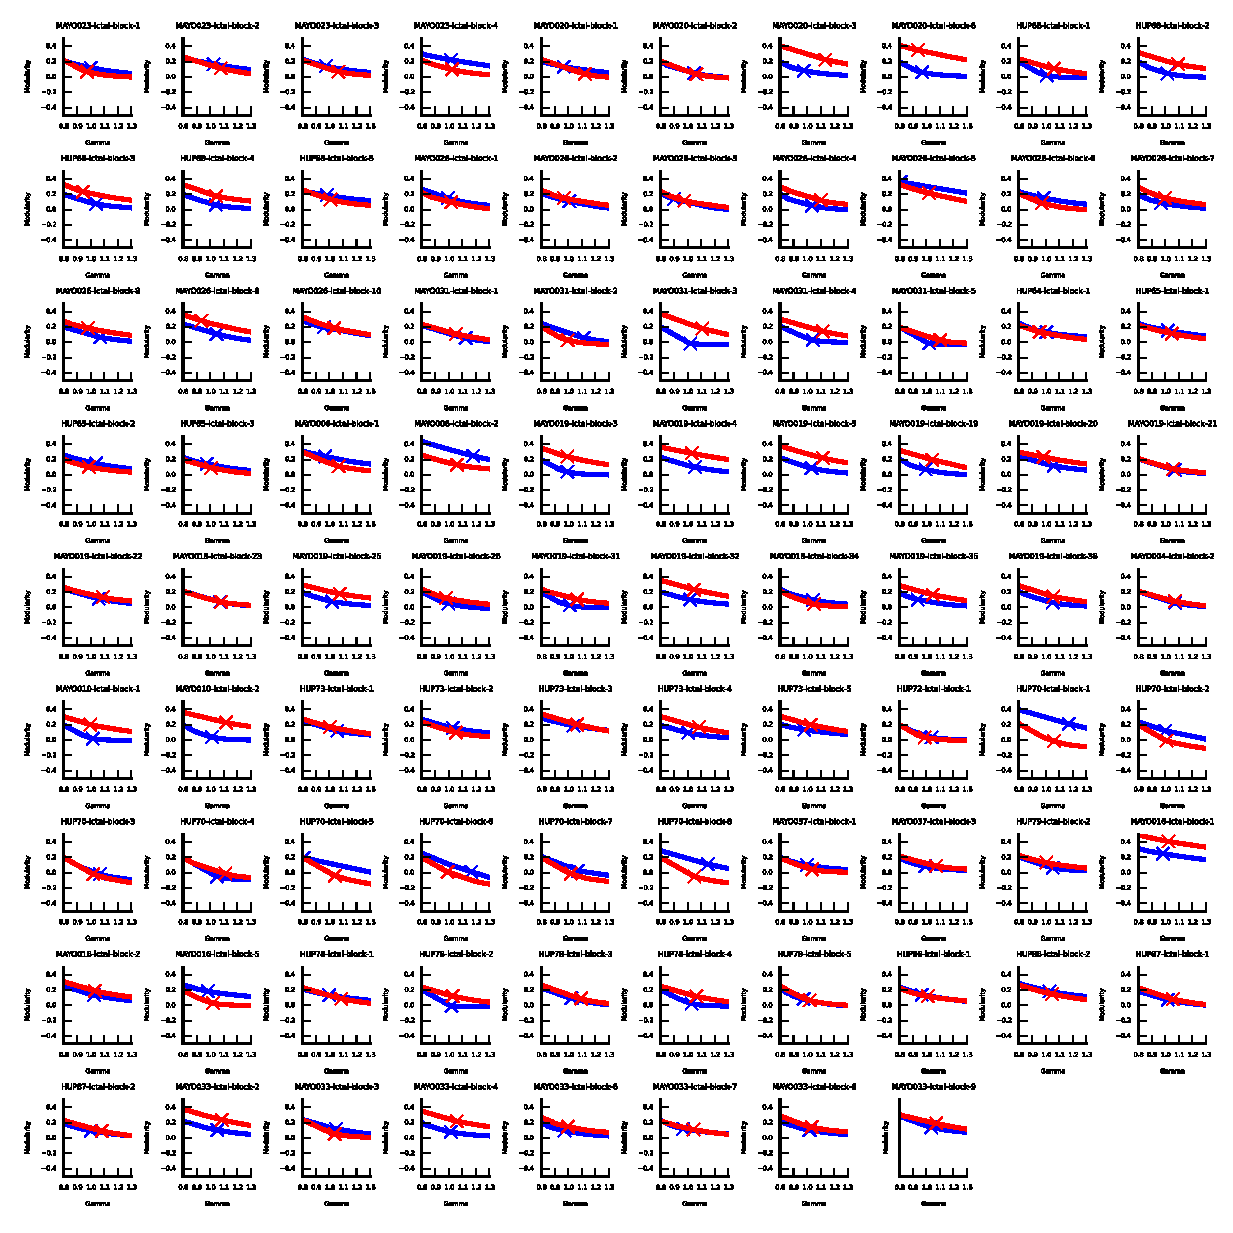
\includegraphics[width=\textwidth]{gammasweep.eps}
    \caption[Structural resolution parameter sweep for modularity optimization]{\textbf{Structural resolution parameter sweep.} Each graph demonstrates the effect of varying $\gamma$ on modularity $\mb{Q}$ per epoch per patient. blue, pre-seizure; red, seizure. Crosses denote the $\gamma$ chosen based on the inflection point for community detection results presented in the main manuscript.\label{ch3:figS1}}
\end{figure}

\begin{figure}[H]
    \centering
    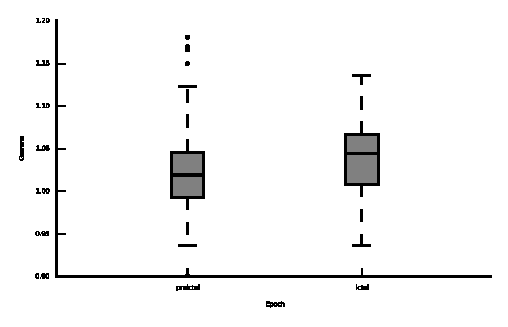
\includegraphics[width=0.5\textwidth]{optgamma.eps}
    \caption[Distribution of optimal structural resolution parameter]{\textbf{Distribution of optimal structural resolution parameter.} Optimal $\gamma$ parameter for pre-seizure and seizure epochs ($N=88$). On average, seizure epochs tend to have more granular temporal division.\label{ch3:figS2}}
\end{figure}

\begin{table}[H]
    \scriptsize
    \centering
    \begin{tabular}{|x{2cm}|x{2.0cm}|x{1.0cm}|x{1.0cm}|x{1.0cm}|x{1.0cm}|x{1.0cm}|x{1.0cm}|}
        \hline
        Patient\newline (IEEG Portal) & Epoch Duration (Sec) & $PS_0$ (sec) & $PS_1$ (sec) & $PS_2$ (sec) & $S_0$ (sec) & $S_1$ (sec) & $S_2$ (sec) \\ \hline \hline
        \verb|HUP64_phaseII| & $107.0\pm0.0$ & $33\pm0.0$ & $31\pm0.0$ & $28\pm0.0$ & $42\pm0.0$ & $37\pm0.0$ & $27\pm0.0$\\ \hline
        \verb|HUP65_phaseII| & $87.7\pm4.5$ & $24.0\pm2.1$ & $17.3\pm3.8$ & $15.0\pm2.5$ & $36.3\pm2.3$ & $27.0\pm0.6$ & $19.3\pm2.7$\\ \hline
        \verb|HUP68_phaseII| & $96.8\pm5.3$ & $32.4\pm6.5$ & $24.8\pm5.2$ & $13.6\pm2.3$ & $32.3\pm4.5$ & $25.8\pm3.5$ & $21.0\pm3.7$\\ \hline
        \verb|HUP70_phaseII| & $107\pm0$ & $4.9\pm0.4$ & $3.8\pm0.5$ & $1.8\pm0.2$ & $6.9\pm0.7$ & $3.0\pm0.4$ & $1.7\pm0.3$\\ \hline
        \verb|HUP72_phaseII| & $90.0\pm0.0$ & $43.0\pm0.0$ & $23.0\pm0.0$ & $20.0\pm0.0$ & $12.0\pm0.0$ & $7.0\pm0.0$ & $6.0\pm0$\\ \hline
        \verb|HUP73_phaseII| & $77.0\pm4.7$ & $23.0\pm7.2$ & $20.2\pm6.3$ & $10.4\pm2.7$ & $33.8\pm2.3$ & $31.2\pm1.8$ & $11.3\pm3.1$\\ \hline
        \verb|HUP78_phaseII| & $46.4\pm6.0$ & $16.6\pm4.6$ & $10.8\pm2.3$ & $7.6\pm1.0$ & $18.2\pm3.2$ & $15.8\pm2.9$ & $4.6\pm1.4$\\ \hline
        \verb|HUP79_phaseII| & $259\pm0.0$ & $96.0\pm0.0$ & $67\pm0.0$ & $59\pm0.0$ & $73\pm0.0$ & $68\pm0.0$ & $45\pm0.0$\\ \hline
        \verb|HUP86_phaseII| & $51.0\pm17.0$ & $21.5\pm3.5$ & $20.5\pm2.5$ & $17.0\pm1.0$ & $19.5\pm8.5$ & $18.0\pm8.0$ & $15.5\pm6.5$\\ \hline
        \verb|HUP87_phaseII| & $10.5\pm1.0$ & $11.5\pm1.5$ & $11.0\pm2.0$ & $5.5\pm0.5$ & $23.5\pm7.5$ & $21.0\pm9.0$ & $3.5\pm2.5$\\ \hline
        \verb|Study 004-2|   & $46.0\pm0.0$ & $9.0\pm0.0$ & $31\pm0.0$ & $28\pm0.0$ & $42\pm0.0$ & $37\pm0.0$ & $27\pm0.0$\\ \hline
        \verb|Study 006|     & $85.0\pm14.0$ & $30.0\pm12.0$ & $26.0\pm13.0$ & $12.5\pm0.5$ & $25.0\pm1.0$ & $18.5\pm2.5$ & $15.5\pm1.5$\\ \hline
        \verb|Study 010|     & $127\pm8.0$ & $38.0\pm5.0$ & $34.0\pm3.0$ & $14.0\pm2.0$ & $35.0\pm9.0$ & $33.0\pm7.0$ & $20.5\pm3.5$\\ \hline
        \verb|Study 016|     & $113\pm18.8$ & $22.7\pm10.2$ & $19.0\pm8.5$ & $12.0\pm6.1$ & $47.7\pm7.2$ & $32.7\pm6.2$ & $17.3\pm8.1$\\ \hline
        \verb|Study 019|     & $116.5\pm16.3$ & $41.3\pm6.2$ & $37.0\pm6.5$ & $13.7\pm2.2$ & $44.3\pm6.3$ & $38.3\pm6.1$ & $22.3\pm4.2$\\ \hline
        \verb|Study 020|     & $64.8\pm25.9$ & $6.8\pm0.5$ & $5.0\pm0.4$ & $3.5\pm0.6$ & $30.5\pm12.4$ & $24.5\pm11.4$ & $6.8\pm3.8$\\ \hline
        \verb|Study 023|     & $64.5\pm11.0$ & $17.3\pm4.7$ & $14.5\pm3.7$ & $11.3\pm2.8$ & $22.5\pm6.9$ & $18.3\pm4.8$ & $8.0\pm0.0$\\ \hline
        \verb|Study 026|     & $53.4\pm2.3$ & $14.2\pm2.3$ & $12.0\pm2.0$ & $7.0\pm1.4$ & $18.3\pm1.3$ & $15.0\pm1.4$ & $10.2\pm1.3$\\ \hline
        \verb|Study 031|     & $44.6\pm3.9$ & $19.2\pm1.1$ & $16.4\pm1.2$ & $6.5\pm3.3$ & $19.0\pm2.9$ & $16.2\pm3.1$ & $5.2\pm1.0$\\ \hline
        \verb|Study 033|     & $118\pm31.4$ & $45.1\pm11.5$ & $39.4\pm9.1$ & $28.0\pm6.9$ & $72.9\pm14.0$ & $60.1\pm9.3$ & $35.6\pm8.5$\\ \hline
        \verb|Study 037|     & $176\pm56.0$ & $31.5\pm25.5$ & $22.0\pm18.0$ & $19.0\pm15.0$ & $79.0\pm20.0$ & $56.5\pm17.5$ & $23.0\pm14.0$\\ \hline
    \end{tabular}
    \caption[Event and state durations for patients]{\textbf{Event and state durations for patients.} Durations of epoch (pre-seizure / seizure) and states are averaged over all events in each patient; $\pm$ represent standard error.\label{ch3:tabS1}}
\end{table}


\chapter{Recurring functional sub-networks during ictal and interictal periods}
\label{ch:mapsubnet}

% the code below specifies where the figures are stored
\ifpdf
    \graphicspath{{chapters/ch4_figures/PNG/}{chapters/ch4_figures/PDF/}{chapters/ch4_figures/}}
\else
    \graphicspath{{chapters/ch4_figures/EPS/}{chapters/ch4_figures/}}
\fi


% ----------------------------------------------------------------------
%: ----------------------- content ----------------------- 
% ----------------------------------------------------------------------
\section{Abstract}
Patients with drug-resistant, neocortical epilepsy suffer from spontaneous seizures, which originate in cortical structures that could also sub-serve normal function. Current clinical practice for localizing seizure-generating brain regions entails monitoring changes from background, interictal patterns of neural activity as seizure begin. A significant challenge with this approach is discerning which cortical pathways lead to seizures and which are important for normal function. We developed a novel technique to disentangle functional sub-networks comprising cohesive cortical pathways from time-varying functional networks constructed from intracranial recordings. Using a consensus clustering scheme, we identified stable clusters of functional pathways expressed during ictal and interictal periods. Our results suggest that cortical pathways involving seizure-onset areas are expressed during both periods and may be predicted by the average strength of connections in the sub-network. Meanwhile, the time-varying expression of cortical pathways from functional sub-networks differentially explains network dynamics during ictal and interictal periods. We found that functional sub-networks are more transiently expressed during ictal periods and more persistently expressed during interictal periods. Collectively, our observations implicate a complex and consistent functional relationship between seizure-generating and ``normal'' structures. Although dysfunction within the epileptic network persists during interictal periods, pathologic regions of the network can be reliably predicted many hours before seizures begin.

\section{Introduction}
For approximately 60 million epilepsy patients, recurring, spontaneous seizures have crippling impact on daily life. In $\approx26\%$ of patients, drivers of seizure activity have been linked to abnormal focal networks located in the neocortex or mesial temporal structures \cite{siegel2001medically}. While the most common treatment strategy is surgical resection to remove cortical tissue generating seizures, newer options such as laser ablation and implantable devices have emerged to selectively target abnormal regions in epileptic networks \cite{fisher2010electrical, morrell2011responsive, tovar-spinoza2013use, medvid2015current}. When discrete lesions coinciding with abnormal electrophysiology are not evident on MRI, only $\approx40\%$ of patients attain seizure freedom following resective surgery. To improve post-surgical outcome, clinicians are increasingly interested in tailoring novel, targeted therapy to affect network regions involved in seizure generation and spread \cite{kutsy1999ictal}. 

To describe mechanisms of seizure generation and evolution, several prior studies have studied the dynamics of epileptic networks, where network nodes are intracranial sensors measuring the electrocorticogram (ECoG) and network connections are statistical relationships between sensors \cite{friston2011functional, hutchison2013dynamic}. Most recent approaches map topologically important network regions within clinically-defined seizure-onset zones and track network dynamics during ictal (seizure) and interictal (normal baseline) epochs \cite{wendling2003epileptic, jerger2005multivariate, schindler2006assessing, schindler2008evolving, kramer2010coalescence, jiruska2012synchronization, burns2014network}. Network hubs of strong connectivity have also emerged adjacent to seizure-onset zones and may localize broader epileptogenic regions \cite{schevon2007cortical, zaveri2009localization-related, rummel2013systems-level, weiss2013ictal, geier2015how}. Together, these studies reveal that network dysfunction underlies complex interactions between drivers of pathologic seizure activity and functional pathways linking cortical regions and that evidence of abnormality exists well before clinically-manifested seizures. This theory aligns well with the popular perspective that the brain is comprised of a number of modular functional sub-networks, recruiting different cortical regions, of which a subset are likely to be expressed at any given time based on functional demand \cite{deco2011dynamical, deco2011emerging, hansen2015functional}. Which begs the following questions: (i) Are functional sub-networks expressed during phases of ictal epochs similar to those expressed during baseline, interictal epochs, and (ii) Do functional sub-networks have a stereotypic pattern of temporal expression that differentiates their mechanism of cortical recruitment between ictal and interictal epochs?
 
In this work, we applied a novel approach for disentangling functional sub-networks and their temporal likelihood of expression to answer the general question: "How are functional pathways differentially expressed during ictal and interictal epochs?" We hypothesize that a common set of cortical pathways underlie functional communication during ictal and interictal epochs, but that the temporal expression of these pathways is different between the two epochs. We posit that stereotypic network architecture might explain why interictal epileptiform activity follows propagation pathways reminiscent to seizure onset and evolution \cite{alarcon1997origin, lai2007cortical, schevon2009spatial, wu2010removing, wilke2009identification,korzeniewska2014ictal}. Therefore, functional sub-networks that connect different cortical regions during normal function may coincide with pathways responsible for seizure initiation and spread. Our results support this hypothesis, demonstrating that functional sub-networks during interictal epochs predict the stereotypic sub-networks expressed during different stages of ictal epochs. Although similar functional pathways phenotype ictal and interictal network architecture, the time-varying expression of sub-networks differentiate the two epochs.

\section{Results}
To disentangle functional sub-networks and their time-varying expression from epileptic brain, we retrieved ECoG recorded during ictal and interictal epochs from 22 neocortical epilepsy patients undergoing routine pre-surgical evaluation of their epilepsy (see \textbf{Table~{\ref{ch4:tab1}}} for patient-specific information) through the \textit{International Epilepsy Electrophysiology Portal} (IEEG Portal, http://www.ieeg.org). We defined an ictal epoch as the period of ECoG signal between -- seizure-onset -- as characterized by the earliest electrographic change (EEC) \cite{litt2001epileptic} -- and seizure termination and an interictal epoch as a continuous 5 minute period of ECoG signal at least 2 hours preceding or following seizure-onset. We analyzed all possible interictal epochs, which amounted to $105\pm17$ hours of ECoG signal per patient.

In each epoch, we estimated weighted functional connectivity using a normalized cross-correlation metric (see \textit{Methods}) applied to non-overlapping, 1s time windows of ECoG (\textbf{Fig.~\ref{ch4:fig1}}). This procedure results in a symmetric, $N \times N$ \textit{connectivity matrix} (specifying $\mfrac{N(N-1)}{2}$ unique connections in the upper or lower triangle of the symmetric connectivity matrix), where $N$ is the number of network nodes, for each of $T$ time windows analyzed. The pattern of unique network connections over all time windows in the epoch is a \textit{configuration matrix} of size $\mfrac{N(N-1)}{2} \times T$.

To extract functional sub-networks from the epileptic network model, we applied a sub-network learning technique called \textit{non-negative matrix factorization (NMF)} to the configuration matrix (see \textit{Methods}). This technique enabled us to soft-partition the time-varying network configuration into modular sub-networks with time-varying expression coefficients. Each sub-network is an additive component of the original network, representing communication pathways between a subset of network regions, that is accompanied by time-varying expression coefficients, measuring the degree to which each sub-network is expressed at a given point in time.

To better understand normal and dysfunctional architecture in the epileptic network, we study the functional sub-networks and time-varying expression coefficients during ictal and interictal epochs.

\begin{table}[H]
    \scriptsize
    \centering
    \begin{tabular}{|x{2cm}|x{0.5cm}|x{0.75cm}|x{2cm}|x{1.5cm}|x{1.25cm}|x{1cm}|x{1cm}|x{1.40cm}|}
        \hline
        Patient\newline (IEEG Portal) & Sex & Age & Seizure Onset & Etiology & Seizure Type & Seizures (N) & Imaging & Outcome \\ \hline \hline
        \verb|HUP64_phaseII| & M & 03/20 & Left frontal & Dysplasia & CP+GTC & 01 & L & ENGEL-I\\ \hline
        \verb|HUP65_phaseII| & M & 02/36 & Right temporal & Auditory reflex & CP+GTC & 03 & N/A & ENGEL-I\\ \hline
        \verb|HUP68_phaseII| & F & 15/26 & Right temporal & Meningitis & CP, CP+GTC & 05 & NL & ENGEL-I\\ \hline
        \verb|HUP70_phaseII| & M & 10/32 & Left perirolandic & Cryptogenic & SP & 08 & L & NR\\ \hline
        \verb|HUP72_phaseII| & F & 11/27 & Bilateral left & Mesial temporal sclerosis & CP+GTC & 01 & L & NR\\ \hline
        \verb|HUP73_phaseII| & M & 11/39 & Anterior right frontal & Meningitis & CP+GTC & 05 & NL & ENGEL-I\\ \hline
        \verb|HUP78_phaseII| & M & 00/54 & Anterior left temporal & Traumatic injury & CP & 05 & L & ENGEL-III\\ \hline
        \verb|HUP79_phaseII| & F & 11/39 & Occipital & Meningitis & CP & 01 & L & NR\\ \hline
        \verb|HUP86_phaseII| & F & 18/25 & Left temporal & Cryptogenic & CP+GTC & 02 & NL & ENGEL-II\\ \hline
        \verb|HUP87_phaseII| & M & 21/24 & Frontal & Meningitis & CP & 02 & L & ENGEL-I\\ \hline
        \verb|Study 004-2|   & F & 14/27 & Right temporal occipital & Unknown & CP+GTC & 01 & NL & ILAE-IV\\ \hline
        \verb|Study 006|     & M & 22/25 & Left frontal & Unknown & CP & 02 & NL & NR\\ \hline
        \verb|Study 010|     & F & 00/13 & Left frontal & Unknown & CP & 02 & L & NF\\ \hline
        \verb|Study 011|     & F & 10/34 & Right frontal & Unknown & CP, CP+GTC & 02 & NL & NF\\ \hline
        \verb|Study 016|     & F & 05/36 & Right temporal orbitofrontal & Unknown & CP+GTC & 03 & NL & ILAE-IV\\ \hline
        \verb|Study 019|     & F & 31/33 & Left temporal & Unknown & CP+GTC & 15 & NL & ILAE-V\\ \hline
        \verb|Study 020|     & M & 05/10 & Right frontal & Unknown & CP+GTC & 04 & NL & ILAE-IV\\ \hline
        \verb|Study 023|     & M & 01/16 & Left occipital & Unknown & CP & 04 & L & ILAE-I\\ \hline
        \verb|Study 026|     & M & 09/09 & Left frontal & Unknown & CP & 10 & NL & ILAE-I\\ \hline
        \verb|Study 031|     & M & 05/05 & Right frontal & Unknown & CP+GTC & 05 & NL & NF\\ \hline
        \verb|Study 033|     & M & 00/03 & Left frontal & Unknown & GA & 07 & L & ILAE-V\\ \hline
        \verb|Study 037|     & F & 45/?? & Indeterminate & Unknown & CP & 02 & NL & NR\\ \hline
    \end{tabular}
    \caption[Patient data set for Chapter \ref{ch:mapsubnet}]{\textbf{Patient information.} Patient data sets accessed through IEEG Portal (http://www.ieeg.org). Age (years) at first reported onset and at phase II monitoring. Localization of seizure onset and etiology is clinically-determined through medical history, imaging, and long-term invasive monitoring. Seizure types are SP (simple-partial), CP (complex-partial), CP+GTC (complex-partial with secondary generalization), or GA (generalized atonic). Counted seizures were recorded in the epilepsy monitoring unit. Clinical imaging analysis concludes L, Lesion; NL, non-lesion. Surgical outcome was based on either Engel score or ILAE score (scale: I-IV/V, seizure freedom to no improvement; NR, no-resection; NF, no follow-up). M, male; F, female. \label{ch4:tab1}}
\end{table}

\begin{figure}[H]
    \centering
    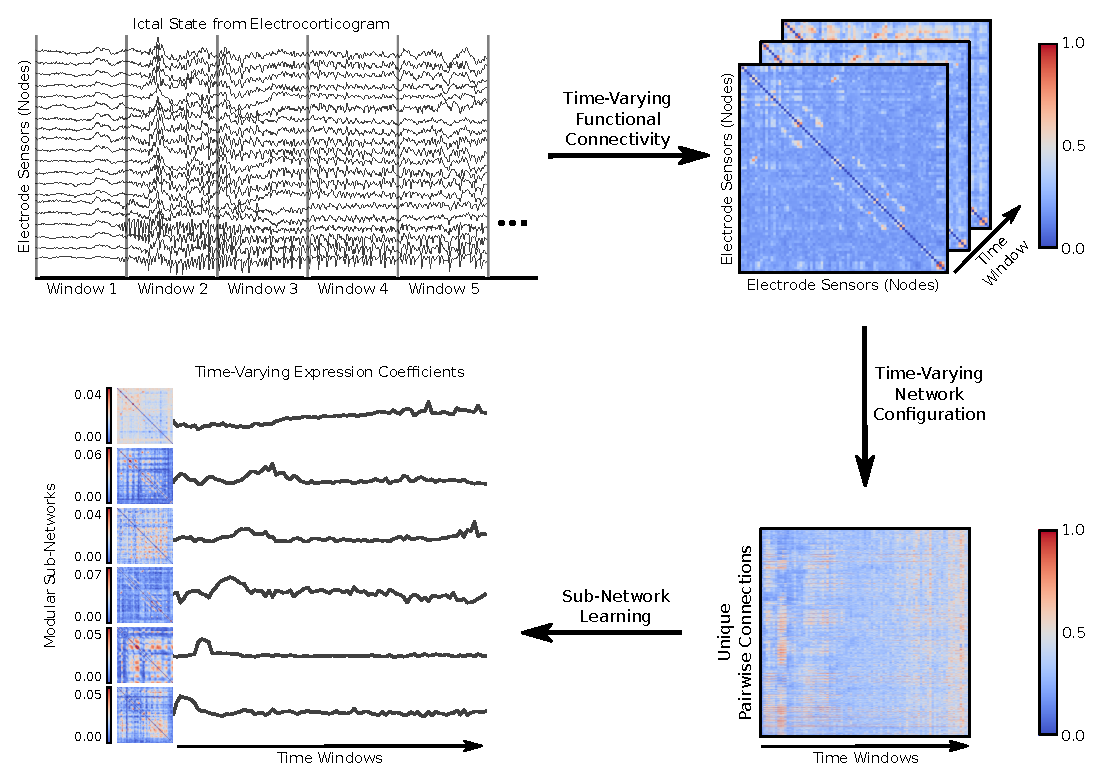
\includegraphics[width=\textwidth]{panel1.eps}
    \caption[Pipeline for disentangling time-varying functional sub-networks]{\textbf{Sub-network learning pipeline for dynamic epileptic networks.} (\textit{Top Left}) We identify ictal and interictal epochs from ECoG signals collected from patients with drug-resistant neocortical epilepsy implanted with intracranial electrodes. An ictal epoch is the period between seizure-onset -- as characterized by the earliest electrographic change (EEC) \cite{litt2001epileptic} -- and seizure termination. An interictal epoch is a continuous, 5 minute period at least 2 hours preceding or following seizure-onset. To measure time-varying functional networks, we divide each epoch into 1s time windows and estimate connectivity in each time window. In our model, each electrode sensor is a network node, and weighted functional connectivity between sensors, interpreted as degree of synchrony, is represented as a network connection. (\textit{Top Right}) For each epoch, we estimated functional connectivity by applying a magnitude normalized cross-correlation between each pair of sensor time series in each time window). (\textit{Bottom Right}) For time-varying functional connectivity, we extract all unique connections between nodes and concatenate over time windows to generate a time-varying network configuration matrix. (\textit{Bottom Left}) We apply \textit{NMF} to the time-varying configuration matrix from each epoch, resulting in a set of co-expressed network regions, sub-networks, with associated expression coefficients for each time window. \label{ch4:fig1}}
\end{figure}

\subsection{Ictal Network Architecture Emerges During Interictal epochs}
Are modular sub-networks expressed during ictal epochs quantifiably similar to those expressed during interictal epochs? To answer this question, we developed a consensus clustering technique to evaluate the degree of similarity between sub-networks of ictal and interictal epochs (see \textit{Methods}). We first generated an ensemble of sub-networks, learned from time-varying functional connectivity of each patient's ictal and interictal epochs. This procedure yielded a patient-specific \textit{ensemble matrix} representing the unique pairwise connectivity between network nodes for every sub-network learned over all epochs (\textbf{Fig.~\ref{ch4:fig2}}). To compute a null distribution of sub-networks for each epoch, we applied a randomly weighted, linear combination of the sub-networks and constructed a \textit{surrogate ensemble matrix}.

Using the true and surrogate ensemble matrices, we next asked whether sub-networks of ictal and interictal epochs reliably cluster together. To test for co-clustering probability between ictal and interictal epochs in each patient, we applied a second stage NMF to the ensemble matrix and tracked the number of times each possible pair of sub-networks were assigned in the same cluster over 100 random initializations. We optimized the number of sub-network clusters per patient by repeating the co-clustering procedure over a range of number of clusters (see \textit{Supplemental Information}). For each patient, this technique yielded a co-clustering probability matrix (\textbf{Fig.~\ref{ch4:fig2}}) capturing the frequency with which pairs of sub-networks over all epochs clustered together. Across the 22 patient cohort, we identified 5 -- 20 clusters consisting of ictal and interictal sub-networks (see \textit{Supplemental Information}). 

\begin{figure}[H]
    \centering
    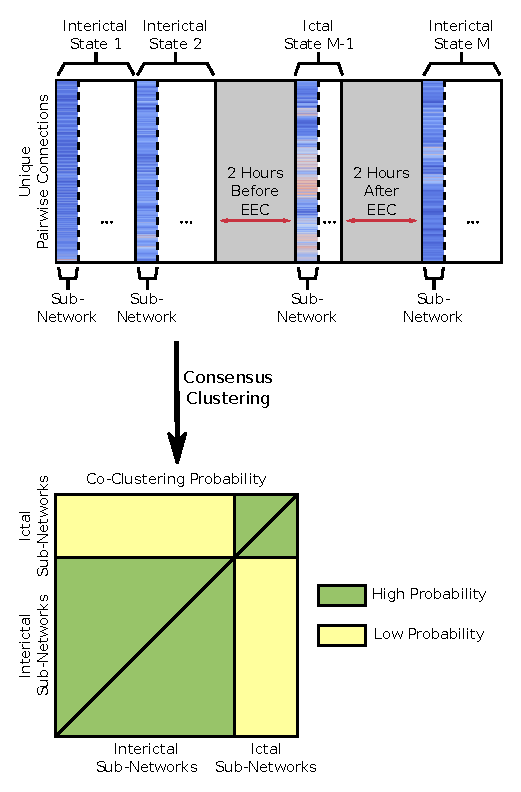
\includegraphics[width=0.5\textwidth]{panel2.eps}
    \caption[Consensus clustering of sub-network ensembles]{\textbf{Consensus clustering for ensemble of sub-networks.} (\textit{Top}) For each patient, we constructed an \textit{ensemble matrix}, representing the $\mfrac{N(N-1)}{2}$ unique connections for each sub-network learned over all ictal and interictal epochs. The ensemble matrix aggregates cortical sub-regions that are expressed during the patients' long-term intracranial recording. We also constructed a \textit{surrogate ensemble matrix} by computing randomly-weighted superposition of sub-networks from each epoch. (\textit{Bottom}) To quantify similarity between cortical sub-regions expressed during interictal and ictal epochs, we employed consensus clustering by applying NMF to the ensemble matrix over a range of number of sub-network clusters each with 100 random initializations. This resulted in a co-clustering probability matrix representing the frequency with which sub-networks from ictal and interictal epochs in the ensemble matrix are clustered together. \label{ch4:fig2}}  
\end{figure}

To analyze the similarity between ictal and interictal sub-networks, we applied multidimensional scaling to project each patient's co-clustering probability matrix on a two-dimensional Euclidean space for true (\textbf{Fig.~\ref{ch4:fig3}A}) and surrogate sub-networks (\textbf{Fig.~\ref{ch4:fig3}B}). This technique projects topographically similar sub-networks closer together (i.e. shorter Euclidean distance). To test whether clusters are significantly more cohesive amongst true sub-networks than surrogate sub-networks, we measured the average Euclidean distance from each sub-network to its cluster centroid, normalized by the distance of the sub-network the population centroid (\textbf{Fig.~\ref{ch4:fig3}C}). Using a One-Way Repeated Measures ANOVA, we found that true clusters are significantly more cohesive than surrogate clusters ($F_{1,21}=1387$, $p<2\times10^{-16}$). This suggests that sub-networks of true clusters are significantly more similar than sub-networks of surrogate clusters. 

Based on our finding of cohesive clustering amongst true ictal and interictal sub-networks, we asked how tightly integrated are ictal sub-networks within their assigned clusters. To quantify cluster integration of ictal sub-networks, as before, we measured the average normalized Euclidean distance from each ictal and interictal sub-network to its cluster centroid, solely for clusters that contained sub-networks of both epochs (\textbf{Fig.~\ref{ch4:fig3}D}). Using a One-Way Repeated Measures ANOVA, we found that ictal sub-networks are significantly more distant from their cluster centroid than interictal sub-networks ($F_{1,21}=11.42$, $p<0.005$). This suggests that ictal sub-networks are less integrated within the cluster than interictal sub-networks. Based on our observation of bridge-like transitions in the two-dimensional projection space of clusters (\textbf{Fig.~\ref{ch4:fig3}A}), we believe ictal sub-networks may represent cortical pathways that lay at the transition between interictal epochs. 

\begin{figure}[H]
    \centering
    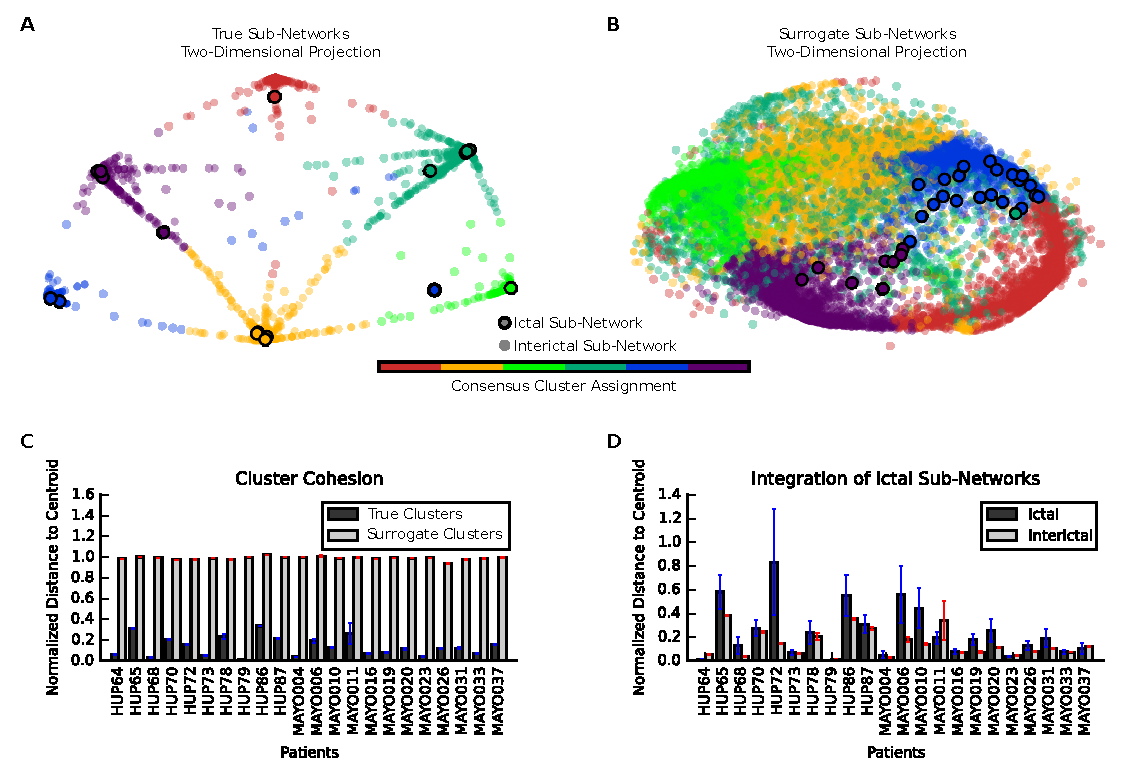
\includegraphics[width=\textwidth]{panel3.eps}
    \caption[Ictal sub-networks recapitulated during interictal epochs]{\textbf{Ictal sub-networks are recapitulated during interictal epochs.} (\textbf{A}) Example two-dimensional projection of one patient's co-clustering probability matrix, where shorter Euclidean distances between circles indicates greater co-clustering probability between expressed sub-networks. Bolded circles represent sub-networks expressed during ictal epochs, and colors represent consensus cluster assignments for each sub-network. (\textbf{B}) Example two-dimensional projection of same patient's surrogate co-clustering probability matrix. The surrogate co-clustering probability matrix, was generated after applying consensus clustering to the surrogate ensemble matrix. (\textbf{C}) Average projection distance from each sub-network to its cluster centroid, normalized by distance to the population centroid, for true and surrogate clusters of each patient. True clusters were significantly more cohesive than surrogate clusters for all 22 patients (One-Way Repeated Measures ANOVA; $F_{1,21}=1387$, $p<2\times10^{-16}$).  (\textbf{D}) Average projection distance from ictal and interictal sub-networks to its cluster centroid, normalized by distance to the population centroid. Ictal sub-networks were significantly further from the cluster centroid than interictal sub-networks (One-Way Repeated Measures ANOVA; $F_{1,21}=11.42$, $p<0.005$) \label{ch4:fig3}}
\end{figure}

\subsection{Interictal Sub-Networks Stereotype Epileptic Network}
In the preceding analyses, we observed that: (i) sub-networks within the same cluster are more similar than sub-networks assigned to other clusters, (ii) ictal sub-networks co-cluster with interictal sub-networks, yet ictal sub-networks tend to be further from the cluster centroid. Next, we investigated to what extent interictal sub-networks can stereotype epileptic network architecture. To address this question, we tested whether interictal sub-networks are capable of predicting pathways related to seizure foci. In accord with routine clinical work-up of patients' epilepsy, a team of neurologists successfully identified the sensors on the seizure-onset zone (SOZ) based on visual inspection of the intracranial recordings. 

We first quantified the extent to which interictal sub-networks express seizure-onset pathways, by computing the \textit{SOZ expression index} as $\mfrac{\bar{C}_\textrm{SOZ}-\bar{C}_\textrm{OUT}}{\bar{C}_\textrm{SOZ}-\bar{C}_\textrm{OUT}}$ -- $\bar{C}_\textrm{SOZ}$ is average connection strength between SOZ nodes in the sub-network and$ \bar{C}_\textrm{OUT}$ is average connection strength between nodes outside the SOZ in the sub-network -- where values range from 0 to 1, representing minimal to strong differential expression between SOZ-SOZ and OUT-OUT connections. To study whether clusters containing interictal sub-networks capture epileptic network architecture, we computed the average SOZ expression index within clusters and sorted the clusters in decreasing order. In an example patient we observed focal expression of SOZ connections in interictal sub-networks with broader expression in ictal sub-networks from the same cluster (\textbf{Fig.~\ref{ch4:fig4}A}). To test whether clusters stereotype interictal sub-networks that express SOZ connectivity, we constructed a linear mixed effects model with no fixed effects and with random effects modeled as intercepts for nested clusters within subjects (\textbf{Fig.~\ref{ch4:fig4}B}). We applied the linear mixed effects model to predict SOZ expression index in true sub-networks and in null sub-networks, where connection strengths within each sub-network were randomly permuted. Using the likelihood ratio test, we found that the observed clusters are more likely to generate true SOZ expression indices ($r^2=0.287$) than null SOZ expression indices ($\tilde{\chi}^2(1)=36091$, $p<2\times10^{-16}$). These results imply that clusters comprised of interictal sub-networks capture network regions involved in seizure-onset, and that some clusters have greater predictive power than others.

While interictal sub-networks can distinguish epileptic network architecture, thus far we only tested the case where we had priori knowledge regarding seizure onset regions. We next asked whether global topological measures can distinctly predict which interictal sub-networks express SOZ connectivity strongly with no prior knowledge of seizure onset regions. To test this hypothesis, we computed and appended the averaged connection strength of each interictal sub-network as a fixed effect to our previous linear mixed effects model (with random effects modeled as intercepts for nested clusters with subjects). Using the likelihood ratio test, we found that the modified linear mixed effects model is significantly more likely to generate the observed values of SOZ expression index than the previous model without fixed effects  ($\tilde{\chi}^2(4)=5952$, $p<2\times10^{-16}$). For our modified model, we evaluated the marginal goodness-of-fit, where average connection strength (fixed effects) alone explain 30.9\%, and the conditional goodness-of-fit, where the full model (fixed effects and random effects) explain 79.6\%, of the overall variance in SOZ expression index amongst interictal sub-networks (\textbf{Fig.~\ref{ch4:fig4}C}). These results presented strong evidence that interictal sub-networks expressing strong SOZ connectivity can be predicted by a global measure of average connection strength. Furthermore, predictability improved by 48.7\% when accounting for clusters of interictal sub-networks that express similar network pathways.

\begin{figure}[H]
    \centering
    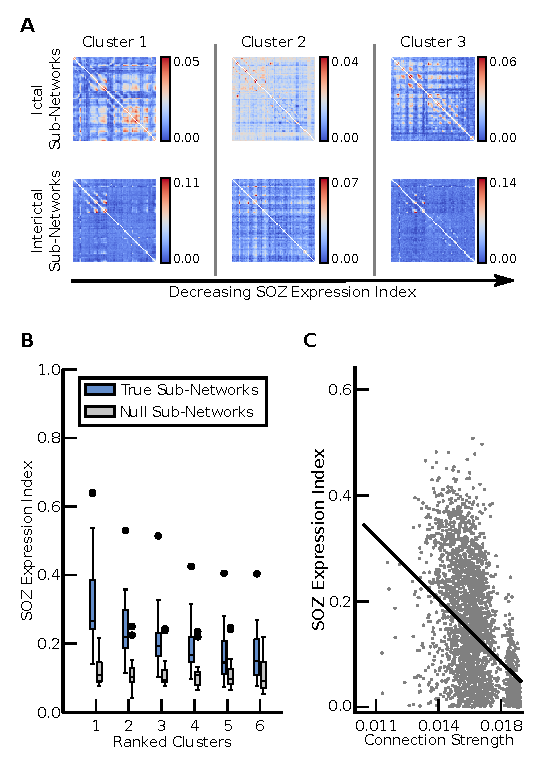
\includegraphics[width=0.5\textwidth]{panel4.eps}
    \caption[Interictal sub-networks predict epileptic network architecture]{\textbf{Interictal sub-networks express emergent architecture of the epileptic network.} (\textbf{A}) First three clusters in order of decreasing SOZ expression index, averaged over all sub-networks within a cluster, for an example patient. Ictal and interictal sub-networks shown are closest to cluster centroids. (\textbf{B}) Distribution of average SOZ expression index over clusters, ranked in decreasing order, from each patient for sub-networks with true (blue) and randomly permuted, null connection strengths (gray). Using a linear mixed effects model to predict SOZ expression index for sub-networks with no fixed effects and with random effects modeled as intercepts for nested clusters within subjects, we found that consensus clusters explain 28.7\% of variance for true SOZ expression index as compared to 17.9\% of variance for null SOZ activation index. (\textbf{C}) Relationship between SOZ expression index and average connection strength in sub-networks from an example patient. Using a linear mixed effects model to predict SOZ expression index with average connection strength as a fixed effect and with random effects modeled as intercepts for nested clusters within subjects, we found that the fixed effects alone explain 29.6\% of the overall variance in SOZ expression index and the full model (fixed effects with random effects) explains 81.4\%. \label{ch4:fig4}}
\end{figure}


\subsection{Functional Sub-Networks Differentially Expressed During Ictal epochs}
We have presented evidence that (i) ictal sub-networks express similar pathways as interictal sub-networks, and (ii) seizure-onset can be predicted by the topology of interictal sub-networks. Logically, we finally ask "If ictal and interictal sub-networks express similar network architecture, how are ictal epochs different from interictal epochs?" 

To answer this question, we analyzed the time-varying expression of sub-networks during ictal and interictal epochs. Based on the understanding that seizures are characterized by a dynamic progression of well-defined epochs, we hypothesized that sub-networks are more transiently expressed, perhaps sequentially, during ictal epochs, and more persistently expressed during interictal epochs. To quantify temporal transience and persistence, we computed the skew of the distribution of time-varying coefficients for each ictal and interictal sub-network, after smoothing with a 5-second moving average filter to reduce spurious noise (\textbf{Fig.~\ref{ch4:fig5}A}). The skew for transient expression was greater than zero, while the skew for persistent expression was less than or equal to zero. Using a One-Way Repeated Measures ANOVA, we found that the skew for ictal time-varying coefficients was significantly greater than for interictal time-varying coefficients ($F_{1,21}=18.81$, $p<0.001$). These results suggest that ictal sub-networks are more transiently expressed than interictal sub-networks, and explains how similar cortical pathways are differentially expressed between ictal and interictal epochs.  

 \begin{figure}[H]
    \centering
    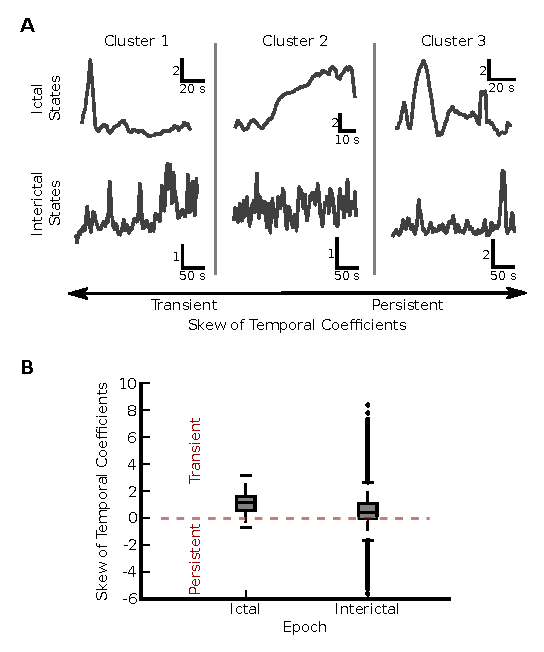
\includegraphics[width=0.5\textwidth]{panel5.eps}
    \caption[Persistent and transient temporal expression of functional sub-networks]{\textbf{Persistent and transient temporal expression differentiates ictal and interictal epochs.} (\textbf{A}) First three clusters in order of increasing skew of temporal coefficients, averaged over all sub-networks within a cluster, for an example patient. Sub-networks with smaller skew in their temporal coefficients are expressed more \textit{persistently} as compared to epochs that are expressed more \textit{transiently}. Temporal coefficients for ictal and interictal sub-networks shown are closest to cluster centroids. (\textbf{B}) Distribution of skew of temporal coefficients for all ictal and interictal sub-networks in an example patient. Using a One-Way Repeated Measures ANOVA, we found that the skew for ictal sub-networks is significantly greater than the skew for interictal sub-networks ($F_{1,21}=18.81$, $p<0.001$). These results suggest that the similar network pathways expressed during ictal and interictal epochs, undergo more transient expression during ictal epochs and are persistent during interictal epochs. \label{ch4:fig5}}
\end{figure}


\section{Discussion}
In this work we asked, "Are similar cortical pathways expressed during ictal and interictal epochs?" To answer this question, we designed and applied a novel tool to disentangle sub-networks and their time-varying expression from dynamic functional connectivity. Our work supports the notion that ictal and interictal epochs traverse a similar set of cortical pathways, but differ in how those pathways are expressed over time. 

\subsection{Modular Cortical Pathways Comprise Epileptic Network Architecture}
A common notion in epilepsy is that isolated cortical regions emit epileptiform activity that can generate seizures. However, network theorists now believe that dysfunction may, in part, arise when epileptiform activity between cortical regions interact, creating the "perfect storm" that leads to seizures. Previous studies have identified discrete network states that describe shifts in the global interactions between all cortical regions \cite{rummel2013systems-level, burns2014network}.  However, these approaches assume that all pathways in the network switch state simultaneously and discretely

Building upon prior work \cite{eavani2013unsupervised, leonardi2013principal, leonardi2014disentangling}, in this study we disentangled the epileptic network into modular sub-networks, or cohesive cortical pathways, that function separately. Logically, different cortical pathways may be variably and continuously expressed to meet functional demand. Our results demonstrated that the epileptic network expresses a small set of functional sub-networks that recur during ictal and interictal epochs. We speculate that the epileptic network consists of stable cortical pathways that contribute to normal function during interictal epochs, and seizure onset and evolution during ictal epochs. Such a theory is corroborated by our finding that these sub-networks are expressed persistently during interictal epochs and transiently during ictal epochs.  


\subsection{Predicting Pathways of the Epileptic Network}
We observed that functional pathways forming the epileptic network are highly predicted by average connection strength and topological clustering of interictal sub-networks. While our results agree with prior studies demonstrating network synchrony is predictive of seizure onset regions during interictal epochs \cite{warren2010synchrony, korzeniewska2014ictal}, we also observed cortical pathways connecting regions outside seizure onset areas that may lead to broader dysfunction \cite{schevon2007cortical, zaveri2009localization-related, weiss2013ictal, rummel2013systems-level}.

Interestingly, these results suggest that functional connectivity linking seizure-onset regions are sustained over long periods of time and persist during functionally normal brain epochs. The appearance of dysfunctional pathways linking cortical regions during interictal epochs can potentially impact cognitive performance in patients with epilepsy. The approach we developed can be used to study looming questions regarding the complex network interactions between epileptic and eloquent cortical regions.

\paragraph{Methodological Limitations and Extensions}
The first important clinical consideration related to this work is the sampling error inherent in any intracranial implantation procedure. Any of the techniques used to map epileptic brain usually yield incomplete representations of the epileptic network. As a consequence, the sub-networks we measured may represent just a portion of larger cortical pathways that extend further throughout the brain.

Secondly, our methods of predicting epileptic network architecture from interictal epochs relies on accurate delineation of seizure-onset regions. Because of sampling error and variability in clinical decision-making, the seizure-onset region may be under or oversampled. However, we believe the high correlation between our model and observed connectivity within seizure-onset regions is reliable based on rigorous statistical testing. Our belief is that unsupervised algorithms to objectively localize network structures may reduce sampling error in the future. 

\subsection{Clinical Impact}
Mapping architecture of the epileptic network presents significant challenges for clinicians. In patients with neocortical epilepsy, we showed that cortical pathways expressed during seizures are highly similar to those pathways traversed during normal function. These findings are relevant for (i) optimizing treatment strategies to reduce dysfunction and preserve normal function and (ii) reducing morbidity and mortality associated with extended duration of invasive intracranial electrode implantation. By predicting seizure-onset regions from interictal epochs, clinical monitoring may be shortened, or potentially even conducted intraoperatively during implant phase. 

\section{Methods}
\subsection{Patient Data Sets}
\subsubsection{Ethics Statement}
All patients included in this study gave written informed consent in accordance with the Institutional Review Board of the University of Pennsylvania.

\subsubsection{Electrophysiology Recordings}
Twenty-two patients undergoing surgical treatment for medically refractory epilepsy believed to be of neocortical origin underwent implantation of subdural electrodes to localize the seizure onset zone after noninvasive monitoring was indeterminate. De-identified patient data was retrieved from the online International Epilepsy Electrophysiology Portal (IEEG Portal) \cite{wagenaar2013multimodal}. ECoG signals were recorded and digitized at either 512 Hz (Hospital of the University of Pennsylvania, Philadelphia, PA) or 500 Hz (Mayo Clinic, Rochester, MN) sampling rate. Surface electrode (Ad Tech Medical Instruments, Racine, WI) configurations, determined by a multidisciplinary team of neurologists and neurosurgeons, consisted of linear and two-dimensional arrays (2.3 mm diameter with 10 mm inter-contact spacing) and sampled the neocortex for epileptic foci (depth electrodes were first verified as being outside the seizure onset zone and subsequently discarded from this analysis). Signals were recorded using a referential montage with the reference electrode, chosen by the clinical team, distant to the site of seizure onset and spanned the duration of a patient's stay in the epilepsy monitoring unit.

\subsubsection{Description of Ictal and Interictal epochs}
Ictal epochs were identified by a team of neurologists as a part of routine clinical work and spanned the period between clinically-marked earliest electrographic change (EEC) \cite{litt2001epileptic} and termination. Interictal epochs spanned 5 minutes in duration and were at least two hours removed from any ictal onset. We analyzed all possible interictal epochs from patient recordings. 

\subsection{Extracting Time-Varying Functional Networks}
Signals from each epoch were divided into $1$-second, non-overlapping, wide-sense stationary time windows in accord with other studies \cite{kramer2010coalescence} and subsequently pre-processed. To test the biasing effect of high-amplitude spiking on signal connectivity measurements, we also investigated windows $0.5$-seconds in duration to sample more of the non-biasing temporal space and found similar results. In each time window, signals were re-referenced to the common average reference \cite{kramer2010coalescence, towle1999electrocorticographic} to account for variation in reference location across patients and to avoid broad field effects that may bias connectivity measurements erroneously in the positive direction. Each window was filtered at 60 Hz to remove line-noise, and low-pass and high-pass filtered at 120 Hz and 1 Hz, respectively, to account for noise and drift. To limit sources of volume conduction from introducing spurious connectivity, we pre-whiten signals in each window using a first-order autoregressive model to account for slow dynamics. This accomplishes two goals: (i) flattening of the signal power spectrum to enhance higher-frequency content that contains local neural population dynamics that is less affected by volume conduction, and (ii) decreases the influence of independent node dynamics when computing correlation-based connectivity measurements \cite{towle1999electrocorticographic, bullmore2001colored, lund2006non-white, arbabshirani2014impact}.

Time-varying functional networks were formed by applying a normalized cross-correlation similarity function $\bs{\rho}$ between the time series of two sensors in the same time window using the formula
    \begin{eqnarray}
        \bs{\rho}_{\mb{xy}}(\mb{k}) = \underset{\tau}{\operatorname{argmax}}\:{\mathrm{E}}[(\mb{x_k}(t) - \mu_{\mb{x_k}})(\mb{y_k}(t+\tau) - \mu_{\mb{y_k}})]
    \end{eqnarray}
    where $\mb{x}$ and $\mb{y}$ are signals from one of $\mb{N}$ sensors or network nodes, $\mb{k}$ is one of $\mb{T}$ non-overlapping, one-second time windows, and $\mb{x_{k}}=\mb{y_{k}}=0$. The $\mb{N}$x$\mb{N}$x$\mb{T}$ similarity matrix is also known as a network adjacency matrix $\mb{A}$. In our weighted network analysis approach, we retain and analyze all possible connection weights between nodes.

\subsection{Learning Functional Sub-Networks}
Sub-networks, or cohesive modules of network pathways, were disentangled from time-varying functional connectivity by clustering the time-varying network configuration matrix through an unsupervised learning algorithm called non-negative matrix factorization (NMF) \cite{lee1999learning}. 

For each ictal or interictal epoch, we constructed the time-varying network configuration matrix $\mb{\hat A}$ by unraveling the upper triangle of $\mb{A}$ resulting in the connection weights of $\mfrac{N(N-1)}{2}$ connections across $\mb{T}$ time windows. Using NMF, we approximated $\mb{\hat A}$ by two low-rank, non-negative matrices, such that:
\begin{eqnarray}
    \mb{\hat A} \approx \mb{W}\mb{H}
\end{eqnarray}
where $\mb{W}$ is the sub-network connectivity matrix (with dimensions $\mfrac{N(N-1)}{2} \times k$), and $\mb{H}$ is the time-varying expression coefficients matrix (with dimensions $k \times T$), and $k$ is the optimized number of sub-networks learned. To compute the NMF, we used the alternating non-negative least squares with block-pivoting method and 200 iterations for fast and efficient factorization of large matrices \cite{kim2011fast} and initialized $\mb{W}$ and $\mb{H}$ using the non-negative double singular value decomposition \cite{boutsidis2008svd}. Given our deterministic initialization for the NMF algorithm, we were guaranteed consistent $\mb{W}$ and $\mb{H}$ on any run -- thus we only performed one run of the NMF algorithm per time-varying network configuration matrix (i.e. one run per ictal or interictal epoch).

For each patient, we determined an optimal number of sub-networks $k$ by the following procedure: (i) randomly sampled 30 epochs from the ictal and interictal pool, (ii) applied NMF for $k$ in the range of 2 to 15 sub-networks independently for each epoch, (iii) computed the Frobenius error between $\mb{\hat A}$ and $\mb{W}\mb{H}$ for each $k$, (iv) retained the value for $k$ that occurs at the elbow of the resulting curve (See \textbf{Fig.~\ref{ch4:figS1}} for distribution of $k$ for each patient), (v) used the average $k$ from 30 epochs as the representative number of sub-networks to learn from all ictal and interictal epochs of the patient. In sum, the sub-network learning procedure yielded $M\times\bar{k}$ total sub-networks per patient, where $M$ is the total number of ictal and interictal epochs. 

\subsection{Consensus Clustering of Sub-Network Ensembles}
Consensus clustering is a general method of testing robustness and stability of clusters over many runs of one or more non-deterministic clustering algorithms \cite{monti2003consensus}. In this work, we studied the nature of clusters amongst the $M\times\bar{k}$ sub-networks per patient. First, we compiled sub-networks from all of a patients' epochs and constructed the ensemble matrix $\mb{E}$ (with dimensions $\mfrac{N(N-1)}{2} \times (M \times \bar{k})$). 

To find consensus clusters in $\mb{E}$, we next applied NMF over 100 runs with matrix factors initialized randomly from a uniform distribution between 0 and 1, such that:
\begin{eqnarray}
    \mb{E} \approx \mb{V}\mb{G}
\end{eqnarray}
where $\mb{G}$ represents the likelihood cluster assignment for each sub-network (with dimensions $j \times (M \times \bar{k})$, where $j$ is the number of patient-wide clusters of sub-networks). After every NMF run, we retrieved the cluster assignment with maximum likelihood for each sub-network and counted the number of times each possible pair of sub-networks was assigned to the same cluster -- and by extension the probability that any two sub-networks co-cluster. These probabilities are tabulated in a symmetric co-clustering probability matrix $\mb{P}$ (with dimensions $(M \times \bar{k}) \times (M \times \bar{k})$). For every patient we repeated this process for a range of $j$ between 5 and 20, and used a proportion of ambiguous clustering (PAC) metric to determine the optimal number of clusters $\bar{j}$ \cite{senbabaoglu2014critical}(see \textbf{Fig.~\ref{ch4:figS2}} for optimal PAC distribution for real and surrogate ensemble matrices). Finally, we assigned each sub-network to its consensus cluster by applying one run of NMF, with $\bar{j}$ clusters, to $\mb{P}$, and retrieving the maximum likely clusters as before (see \textbf{Fig.~\ref{ch4:figS3}}). As suggested by previous work, $\mb{P}$ is a similarity matrix \cite{monti2003consensus} that we used to analyze and visualize sub-network clustering via multi-dimensional scaling methods \cite{borg2005modern}. 

\section{Acknowledgments}
AK and BL acknowledge support from the National Institutes of Health through awards \#R01-NS063039, \#1U24 NS 63930-01A1, the Citizens United for Research in Epilepsy (CURE) through Julie's Hope Award, and the Mirowski Foundation. DSB acknowledges support from the John D. and Catherine T. MacArthur Foundation, the Alfred P. Sloan Foundation, the Army Research Laboratory, the Institute for Translational Medicine and Therapeautics, the National Institute of Mental Health through award number 2-R01-DC-009209-11 (Thompson-Schill), and the National Science Foundation awards CRCNS BCS-1441502 and BCS-1430087 through the ENG, CISE, and SBE directorates. The content is solely the responsibility of the authors and does not necessarily represent the official views of any of the funding agencies.

\begin{figure}[H]
    \centering
    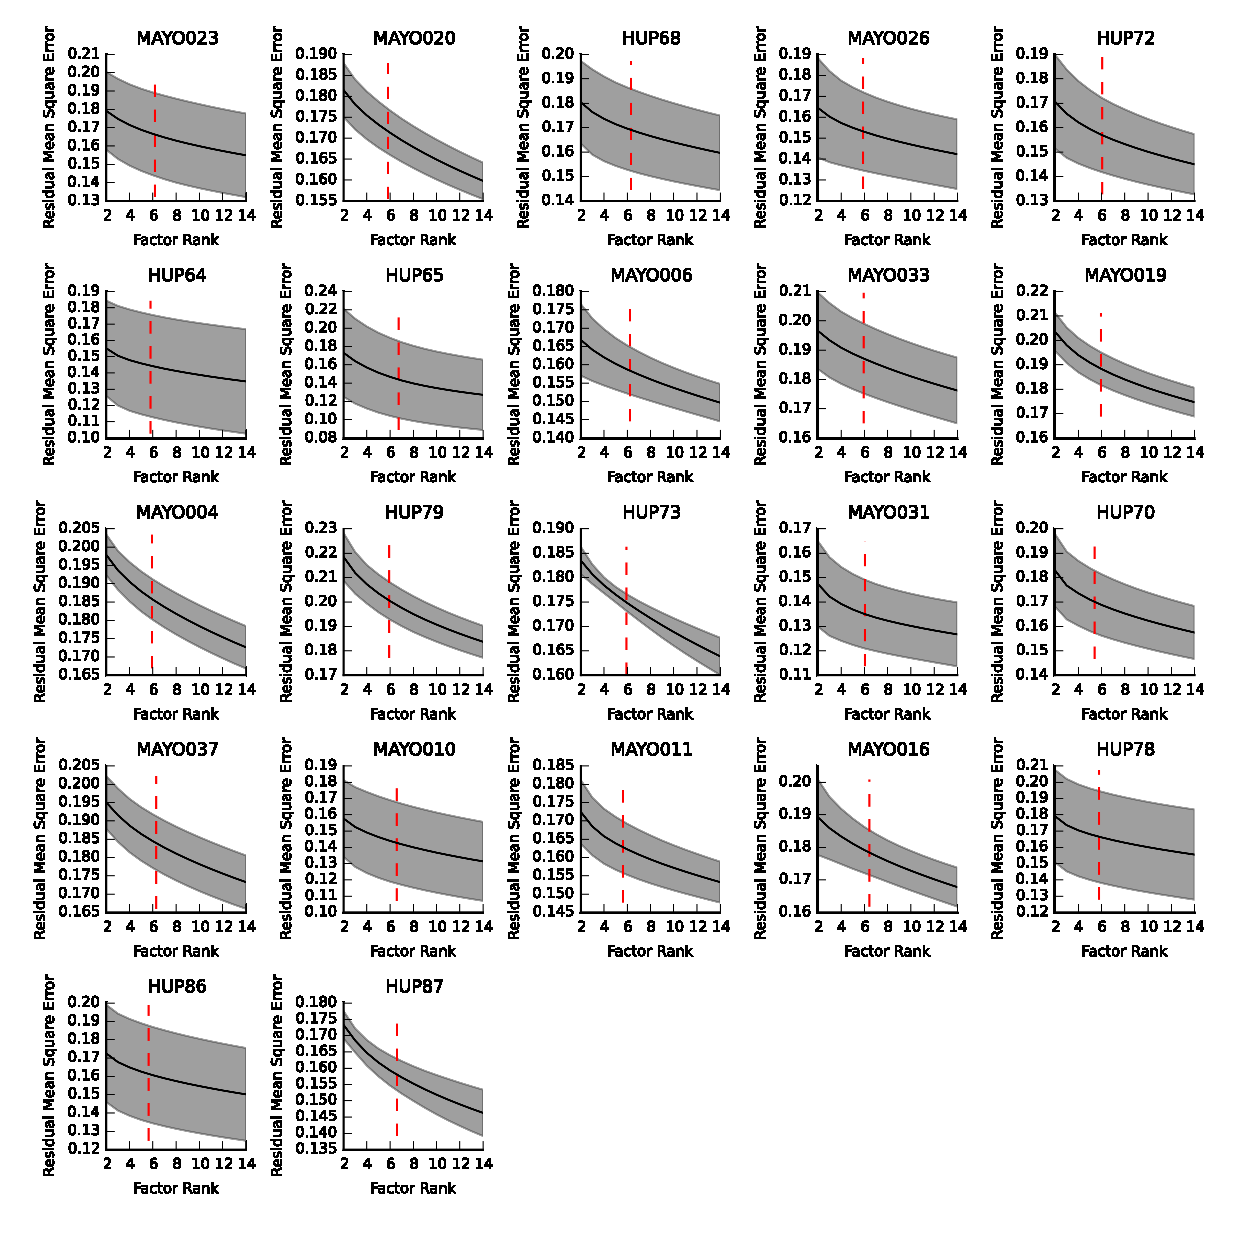
\includegraphics[width=\textwidth]{NMF_factor_optimization.eps}
    \caption[Optimizing number of learned sub-networks]{\textbf{Optimizing number of learned sub-networks.} For each patient, we analyzed the distribution of Frobenius normed error between the network configuration matrix $\mb{\hat A}$ and the learned sub-networks $\mb{W}\mb{H}$ in 30 randomly sampled ictal or interictal epochs. Each graph represents the distribution of error as a function of the number of sub-networks learned $k$. The mean (black) and $\pm1$ standard deviation (gray) over the 30 epochs are plotted. The optimal number of sub-networks $\bar{k}$ for each patient was computed to be the elbow of this curve (dashed red line). \label{ch4:figS1}}    
\end{figure}

\begin{figure}[H]
    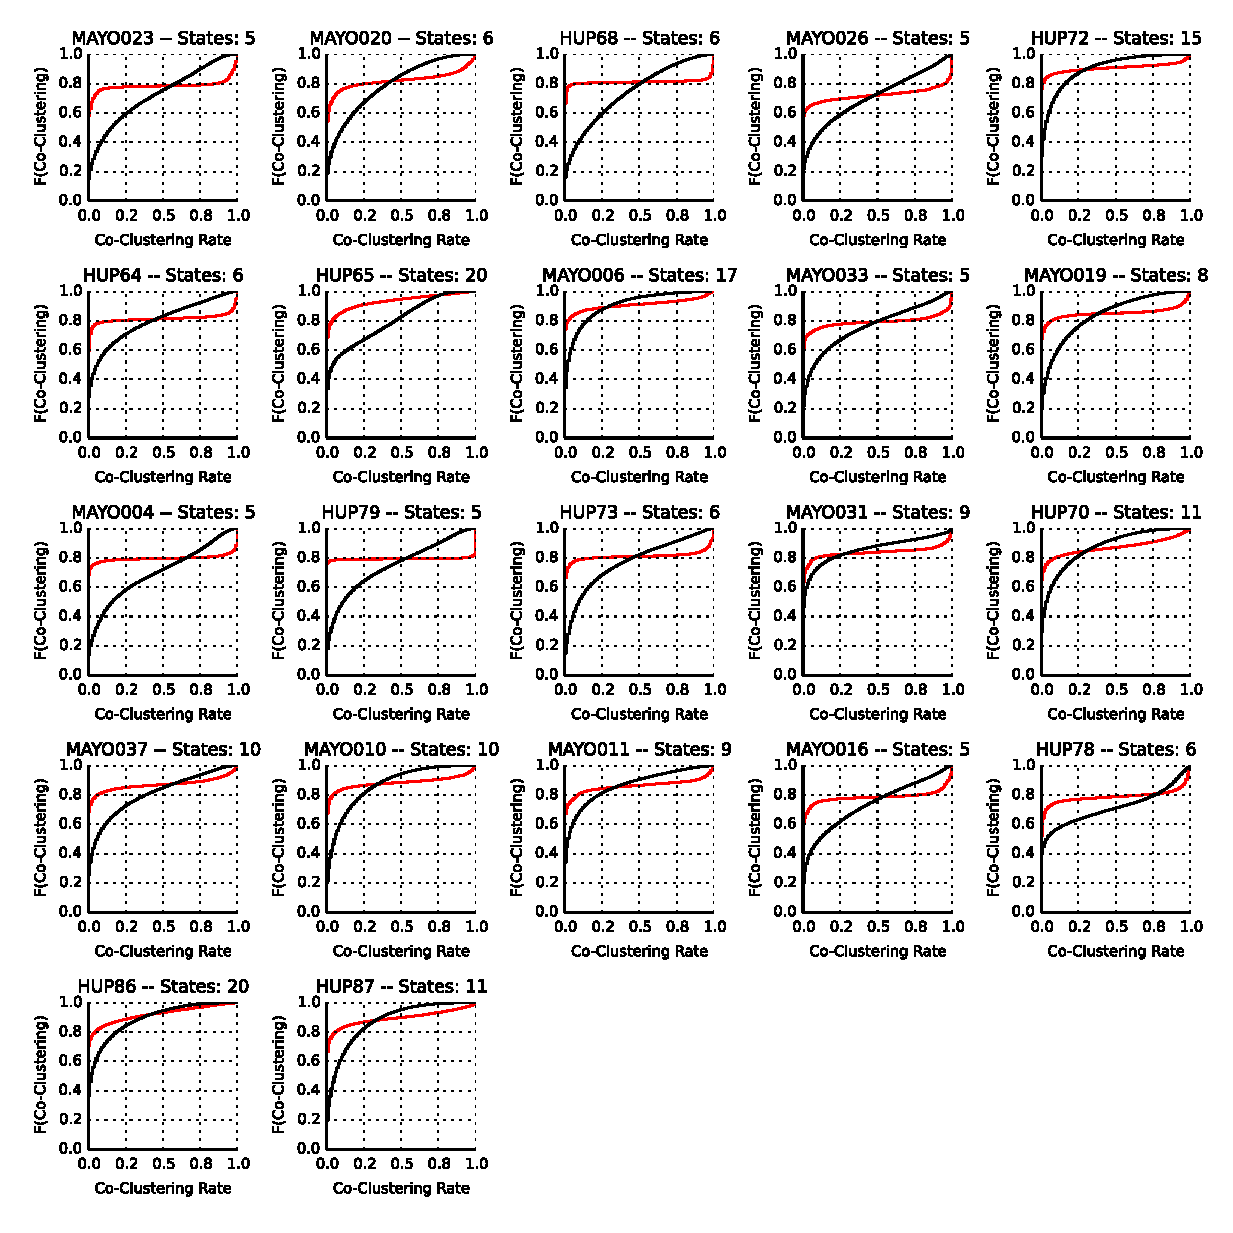
\includegraphics[width=0.9\textwidth]{patient_stateNMF_cdf_pac.eps}
    \caption[Optimizing number of consensus clusters from sub-network ensemble]{\textbf{Optimizing number of consensus clusters from sub-network ensemble.} For each patient, we computed co-clustering probability matrices for a range of number of consensus clusters $j$. To optimize the number of consensus clusters, we computed a cumulative distribution function (CDF) of co-clustering probability for each $j$, quantified the proportion of ambiguous clusters (PAC) as given by $\text{CDF}_j(0.9)-\text{CDF}_j(0.1)$, and retained $\bar{j}$ that resulted in the minimum PAC. The CDF for the optimum number of clusters $\bar{j}$ in red. The CDF for the same number of clusters for the surrogate co-clustering probability matrix is in black. We observed more clustering ambiguity in the surrogate population than the real population. \label{ch4:figS2}}
\end{figure}

\begin{figure}[H]
    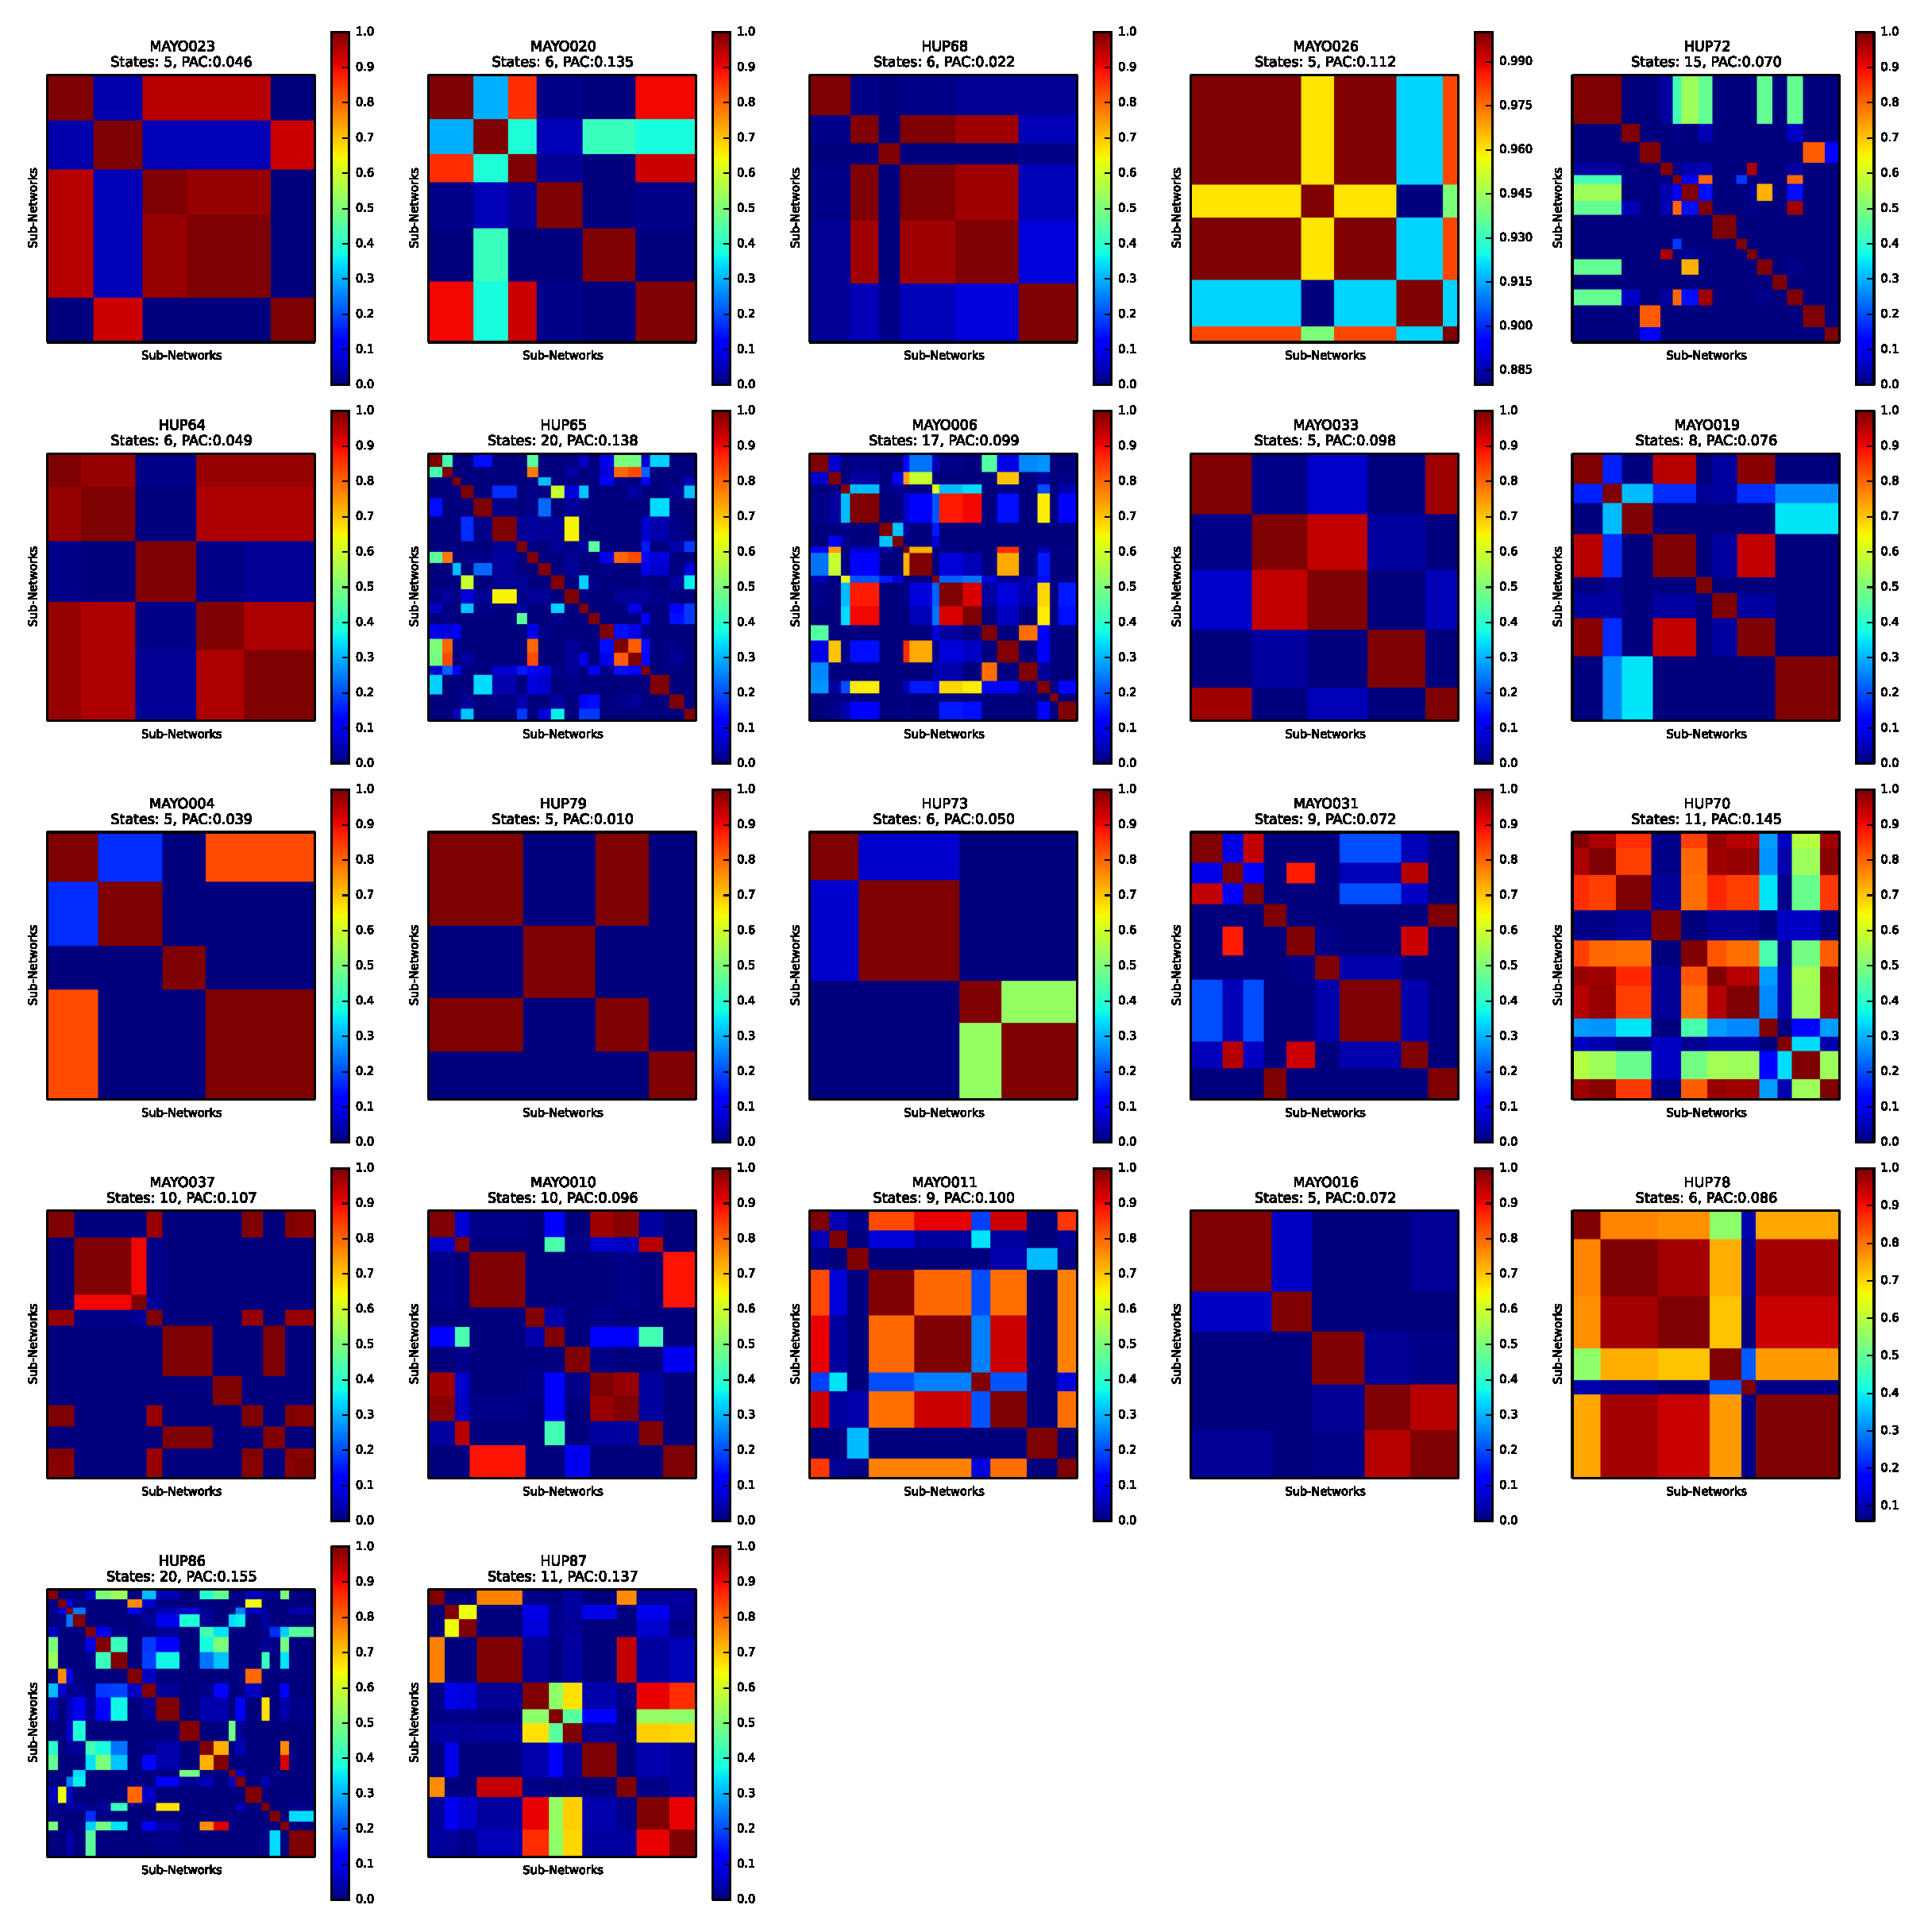
\includegraphics[width=\textwidth]{assign_true_cluster.eps}
    \caption[Co-clustering probability of ictal and interictal sub-networks]{\textbf{Optimum co-clustering probability of sub-networks.} For each patient, we assigned each ictal and interictal sub-network to a consensus cluster and re-ordered the co-clustering probability based on assigned clusters. We observed high co-clustering probability between clusters of sub-networks (block diagonal elements) and low co-clustering probability between clusters (off-diagonal blocks). \label{ch4:figS3}}
\end{figure}

\chapter{Virtual cortical resection reveals push-pull network control mechanism}
\label{ch:selfreg}

% the code below specifies where the figures are stored
\ifpdf
    \graphicspath{{chapters/ch5_figures/PNG/}{chapters/ch5_figures/PDF/}{chapters/ch5_figures/}}
\else
    \graphicspath{{chapters/ch5_figures/EPS/}{chapters/ch5_figures/}}
\fi


% ----------------------------------------------------------------------
%: ----------------------- content ----------------------- 
% ----------------------------------------------------------------------
\section{Abstract}
For $\approx$20 million people with drug-resistant epilepsy, recurring, spontaneous seizures have devastating impact on daily life. Current treatment options for these patients are resective surgery, and more recently, implantable devices to control seizures. The efficacy of these therapies is hindered by a poor understanding of why some seizures spread to surrounding tissue while others remain focal and confined. Network mechanisms that regulate synchronization between connected brain regions may explain differential seizure dynamics. To pinpoint network regions that regulate seizure evolution, we present a novel method to assess changes in synchronizability in response to virtually lesioning cortical areas in a validated computational network model. We apply our virtual cortical resection technique to time-varying functional networks measured in 10 human patients implanted with electrocorticographic sensors for clinical localization of their epilepsy. Our results suggest that the network's synchronizability prior to seizure onset predicts the extent of seizure evolution. Using virtual cortical resection, i.e. selectively removing nodes from the computational model, we identify important control regions that drive network behavior by individually desynchronizing or synchronizing distinct cortical areas. We find that for seizures that remain focal, the strongest controllers preceding seizures are localized outside seizure-generating areas. Our results support the notion that these controllers utilize an antagonistic push-pull control scheme to regulate network synchronizability. These studies suggest that tailoring therapy to leverage regulatory mechanisms that constrain the extent of seizure spread may improve existing treatment. 

\section{Introduction}
Functional architecture of the epileptic neocortex has been studied extensively to better identify optimal targets for surgical resection and, more recently, the optimal location for implantable devices. The prospect of patient-centric algorithms that modulate brain state to abort seizures is exciting to clinicians and researchers alike \cite{morrell2011responsive, stanslaski2012design, afshar2013translational}. However, the best targets for chronic devices remain elusive, partly because functional brain networks, including epileptic networks, reorganize dynamically \cite{bassett2006adaptive, bassett2011dynamic, rummel2013systems-level, burns2014network}. Such reorganization appear to follow a specific progression through network states unique to the patient's seizures \cite{wulsin2013parsing, burns2014network}. The mechanisms that drive seizures through network states can inform neural control paradigms that aim to stop or contain propagation of seizure activity. Such a capability is vital, clinically, because epileptogenic regions cause symptoms not only through their own dysfunction, but also through their ability to recruit and disrupt normal brain regions \cite{kutsy1999ictal}. However, understanding and translating network mechanisms of seizure evolution to identify targets for therapy requires further dissection of functional epileptic network architecture. 

Conventional school of thought divides epileptic brain into the \textit{seizure-onset} or \textit{ictal zone}, a clinically-defined where seizures are generated, and the \textit{irritative zone}, which emits non-seizure-generating epileptiform events including spike-wave discharges and high-frequency oscillations \cite{rosenow2001presurgical}. Recent models describe connectivity between the seizure-onset and irritative zones in the framework of a broader dysfunctional \textit{epileptic network}, where network nodes are neural populations measured by intracranial sensors and network connections are statistical relationships between neural activation patterns \cite{nair2004critical, kramer2010coalescence, warren2010synchrony, wilke2011graph, burns2014network} (\textbf{Fig.~\ref{ch5:fig1}A}). For example, partial seizures that begin in the seizure-onset zone can evolve, spreading spatially as they modulate in dominant frequency, via local connections to the surrounding tissue, implicating a distributed epileptic network \cite{spencer2002neural, nair2004critical, kramer2010coalescence, korzeniewska2014ictal}. In the extreme case these seizures secondarily generalize to encompass the entire brain.

Given the distributed nature of epileptic activity, it is critical to isolate underlying propagation mechanisms. Leading hypotheses suggest that either (i) seizure evolution is driven by strong, synchronizing activity from the seizure-generating network impinging outward on the surrounding tissue \cite{schindler2008evolving, kramer2010coalescence, kramer2012epilepsy, jiruska2012synchronization}, or (ii) seizure evolution is caused by a diminished ability of the surrounding tissue to regulate, or contain, abnormal activity \cite{nair2004critical, bower2012spatiotemporal}. While little evidence exists to determine which of these hypotheses accurately reflect seizure dynamics, both mechanisms can be succinctly summarized as abnormalities of synchronizability, a description of how easily neural processes, such as rhythmic activity, can flow through a network.

Theoretical work demonstrates that the synchronizability of a system can be regulated through a \textit{push-pull control} mechanism, where desynchronizing and synchronizing nodes operate antagonistically in a ``tug-of-war'' to maintain network stability. When desynchronizing, synchronizing or both forces weaken, network stability is compromised such that the network is driven to a different state \cite{he2014control} (\textbf{Fig.~\ref{ch5:fig1}B}). Such mechanisms are particularly successful in heterogeneous networks like the brain, where some nodes are sparsely connected and other nodes are densely connected \cite{wang2002synchronization}. Does the brain utilize such a control mechanism for seizure regulation? And if so, what regions of the brain affect this control?

To address these questions, we present a novel method we call \textit{virtual cortical resection}, which offers a statistically robust means to pinpoint putative control nodes in the epileptic network that may regulate seizure dynamics, based on the network's response to virtual lesioning \cite{wang2002synchronization, wang2002pinning}. We use this method to test the hypothesis that the epileptic network contains a native regulatory system (\textbf{Fig.~\ref{ch5:fig1}C}) whose connectivity to the seizure-generating area accounts for differential seizure dynamics, including (i) the constrained dynamics observed in partial seizures that remain focal (\textbf{Fig.~\ref{ch5:fig1}D}), and (ii) the unconstrained dynamics observed in partial seizures that generalize to surrounding tissue (\textbf{Fig.~\ref{ch5:fig1}E}).

More specifically, using electrocorticography recorded from 10 patients diagnosed with drug-resistant neocortical epilepsy undergoing routine pre-surgical evaluation, we constructed time-evolving functional networks across \emph{events}, each of which included a seizure epoch preceded by a pre-seizure epoch. The seizure epoch spanned the period between the clinically-marked earliest electrographic change \cite{litt2001epileptic} and the seizure termination, while the pre-seizure epoch was identical in duration to the seizure and ended immediately prior to the earliest electrographic change. In each epoch we divided the ECoG signal into 1s non-overlapping time-windows and estimated functional connectivity in a high-$\gamma$ (95--105 Hz) frequency band using multitaper coherence estimation (see \textit{Methods}). We implemented virtual cortical resection on this dynamic epileptic network by independently removing electrode sites from the network model. This was done to assess the synchronizability of (i) the distributed epileptic network in partial seizures that generalize to surrounding tissue, \emph{versus} (ii) the focal epileptic network in those that do not. By removing electrode sites from the network model, we were able to probe the importance brain regions, in their presence and absence, to seizure generation and propagation.

\begin{figure}[H]
    \centering
    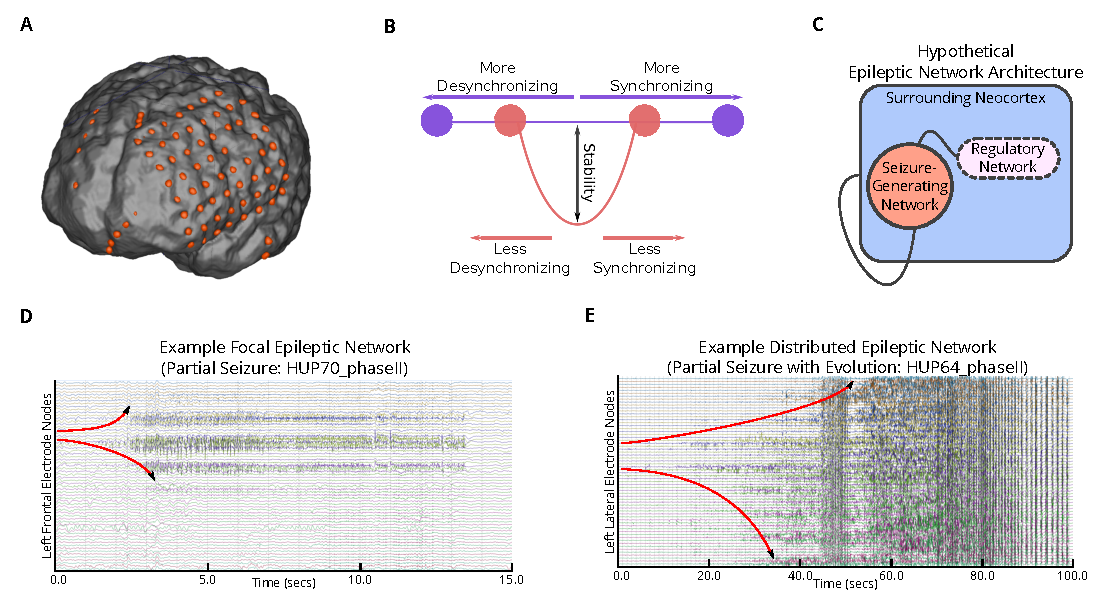
\includegraphics[width=\textwidth]{panel1.eps}
    \caption[Hypothetical regulatory mechansim of seizure spread]{\textbf{Hypothesized regulatory mechanism of seizure spread} (\textbf{A}) We create functional networks based on electrophysiology from patients with drug-resistant neocortical epilepsy implanted with intracranial electrodes. Each sensor is represented as a network node, and weighted functional connectivity between sensors, interpreted as degree of coherence, is represented as a network connection. (\textbf{B}) Rope-stretching diagram demonstrating push-pull control, where greater antagonism between opposing synchronizing and desynchronizing forces (nodes) improves rope-tightness (network stability) in the blue rope compared to the red rope. (\textbf{C}) Schematic of the epileptic network composed of a \textit{seizure-generating system} and a hypothesized \textit{regulatory system} that controls the spread of pathologic seizure activity. (\textbf{D}) Example partial seizure that remains focal: the seizure begins at a single node and evolves to and persists within a focal area. (\textbf{E}) Example partial seizure that generalizes to surrounding tissue: the seizure begins at two nodes and evolves to the broader network. We hypothesize that these two types of dynamics are determined by differences in the regulatory system. \label{ch5:fig1}}
\end{figure}


\section{Results}

\subsection{Network Heterogeneity Drives Global Synchronizability}
We first asked the question, ``Does the distributed epileptic network have an increased potential to synchronize compared to the focal epileptic network?'' We hypothesized that networks with a more heterogeneous distribution of node strengths would have a weaker synchronizability. To measure heterogeneity, we computed a non-parametric, normalized measure of node strength dispersion $d(t)$ for each time-window $t$ (see \textit{Methods}). The focal network displayed a significantly greater dispersion than the distributed network during the pre-seizure epoch but not during the seizure epoch (\textbf{Fig.~\ref{ch5:fig2}A}). These results suggest that greater heterogeneity in high-$\gamma$ networks precedes partial seizures that do not generalize to the surrounding tissue.

To determine whether network heterogeneity corresponds to decreased synchronizability, we estimated the time-varying Laplacian matrix $\textbf{L}(t)$ whose entries $l_{ij}(t)$ quantify how easily information can diffuse between nodes $i$ and $j$ (see \textit{Methods}). Next, we computed the network synchronizability $s_{t}=\frac{\lambda_2}{\lambda_\text{max}}$, where $\lambda_2$ and $\lambda_\text{max}$ are the second-smallest eigenvalue and the largest eigenvalue, respectively, of $\textbf{L}(t)$ (see \cite{barahona2002synchronization} and \textbf{Supplementary Note}). We observed significantly greater synchronizability in the distributed epileptic network than in the focal epileptic network during the pre-seizure epoch, suggesting that high-$\gamma$ networks have a greater potential to synchronize preceding partial seizures that generalize to surrounding tissue (\textbf{Fig.~\ref{ch5:fig2}B}). In contrast, we observed no significant differences in the synchronizability during the seizure epoch, suggesting that both the focal and distributed epileptic networks have similar synchronizability. Finally, we observed that high heterogeneity corresponds to low synchronizability in the pre-seizure epoch, suggesting that the heightened influence of a subset of network nodes hampers the network's ability to synchronize. More generally, these results suggest that network heterogeneity in the distributed epileptic network may reflect a fundamental vulnerability to synchronize easily, a vulnerability that is not present in partial seizures that do not generalize to surrounding tissue.

\begin{figure}[H]
    \centering
    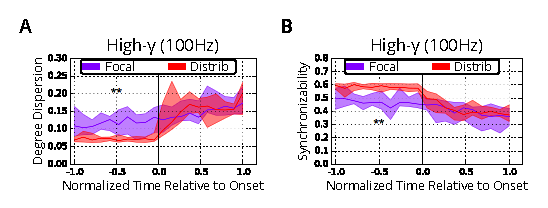
\includegraphics[width=\textwidth]{panel2.eps}
    \caption[Global synchronizability predicts seizure evolution]{\textbf{Differential pre-seizure synchronizability predicts seizure evolution.} (\textbf{A}) Heterogeneity, as measured by time-dependent dispersion of node strength in high-$\gamma$ functional networks, differed significantly in (i) partial seizures that remain focal ($N=19$), compared to (ii) partial seizures that generalize to surrounding tissue ($N=16$): (FDA, $p_\text{pre-seizure}=1.8\times10^{-4}$, $p_\text{seizure}=8.1\times10^{-1}$. (\textbf{B}) Time-dependent synchronizability in high-$\gamma$ functional networks differs significantly in the two types of seizures: (FDA, $p_\text{pre-seizure}=4.1\times10^{-4}$, $p_\text{seizure}=1.7\times10^{-1}$). Thick lines represent median, shaded area represents $1^{st}$ and $3^{rd}$ quartile. $P$-values are obtained via functional data analysis (FDA) where event labels (two seizure types) were permuted uniformly at random (see Methods): *$p<0.05$, **$p<0.001$. \label{ch5:fig2}}
\end{figure}


\subsection{Network Controllers of Synchronizability}
How might network heterogeneity regulate levels of synchronizability? Do a subset of nodes act as key controllers, or do all nodes contribute equally? To answer this question, we developed a novel method to assess the influence of a node on synchronizability. We define the \emph{control centrality} $c_i$ of node $i$ to be the fractional change in synchronizability following removal of node $i$ from the network (\textbf{Fig.~\ref{ch5:fig3}A}): $c_i=\frac{s_i-s}{s}$ where $s$ is the original synchronizability and $s_i$ is the synchronizability after node removal. The magnitude of $c_i$ can be interpreted as the overall strength of the node as a controller of synchronizability. If $c_i$ is positive, then synchronizability increases upon node removal, and the node is said to be a \emph{desynchronizing node}. If $c_i$ is negative, then synchronizability decreases upon node removal, and the node is said to be a \emph{synchronizing node}. As illustrated in \textbf{Fig.~\ref{ch5:fig3}A}, both desynchronizing and synchronizing network controllers are characteristic of heterogeneous networks, and tend to be located in the network periphery and network core, respectively.

\begin{figure}[H]
    \centering
    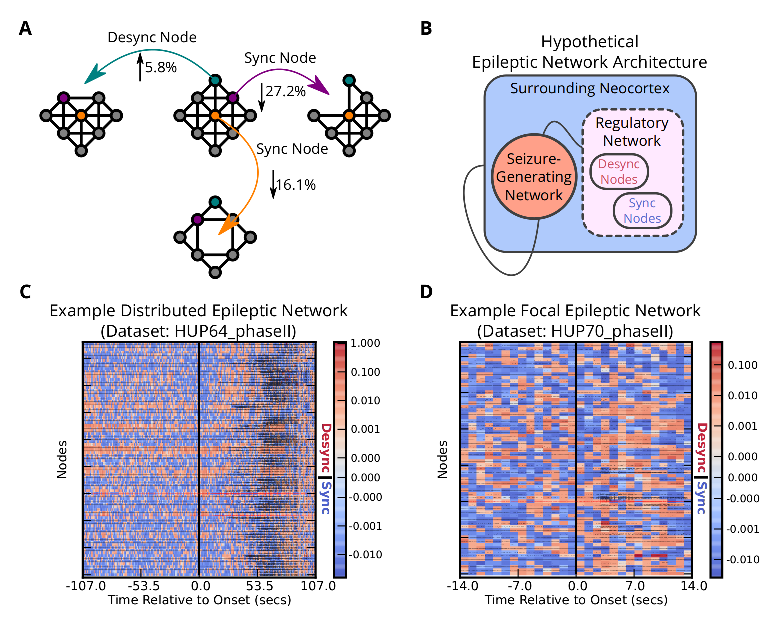
\includegraphics[width=\textwidth]{panel3.eps}
    \caption[Schematic of virtual cortical resection]{\textbf{Virtual cortical resection localizes network controllers.} (\textbf{A}) Effect of node removal on network synchronizability (control centrality) in a toy network. Highlighted node removals resulting in increased synchronizability (desynchronizing node; blue), decreased synchronizability (synchronizing nodes; purple and orange). The strongest desynchronizing node increased synchronizability by 5.8\% and was present in the network periphery, while the strongest synchronizing nodes decreased synchronizability by 27.2\% and 16.1\% and were located in the network core. (\textbf{B}) Hypothetical regulatory network employs desynchronizing and synchronizing nodes to regulate levels of synchronizability. (\textbf{C}) Control centrality in example distributed (and (\textbf{D}) focal) epileptic network events. ECoG signal is normalized by maximum amplitude. Red signals signify clinically-marked seizure-generating nodes. \label{ch5:fig3}}
\end{figure}

We used control centrality to assess the presence of desynchronizing and synchronizing controllers in the epileptic network, and to define their putative role in regulating synchronizability, a hallmark of seizure dynamics (\textbf{Fig.~\ref{ch5:fig3}B}). We observed that controller roles differed in their temporal dynamics, and in spatial distribution. In an example of a distributed epileptic network (see \textbf{Fig.~\ref{ch5:fig3}C}), we found clusters of desynchronizing nodes that switched to synchronizing nodes as the seizure began (and desynchronizing controllers appear elsewhere), and then switched back to desynchronizing nodes as the seizure terminated (and synchronizing controllers appear elsewhere). Interestingly, these coordinated dynamics occurred away from seizure-generating areas. In an example of a focal epileptic network (see \textbf{Fig.~\ref{ch5:fig3}D}), we observed less coordinated dynamics; preceding the seizure, desynchronizing and synchronizing controllers appeared dispersed across the network, while, after seizure-generation, more apparent clustering of desynchronizing and synchronizing nodes emerged away from the seizure-generating areas (see for example \textbf{Fig.~\ref{ch5:fig3}D}).

\subsection{Regulatory System Controls Seizure Dynamics}
Given that synchronizability appears to be driven by a small number of synchronizing and desynchronizing nodes in the tissue surrounding the seizure-generating area, we next asked whether these putative controllers displayed differential influence in different seizure types. To address this question, we separately computed the average of the control centrality over all time-windows in each epoch for the seizure-generating area and the surrounding tissue. In the seizure-generating area, we found no differences in the control centrality estimated during the pre-seizure epoch for the partial seizures that remained focal in comparison to the partial seizures that generalized to surrounding tissue. In contrast, in the surrounding tissue, we observed significantly greater control centrality in the focal in comparison to the generalized case (\textbf{Fig.~\ref{ch5:fig4}A}). No differences in control centrality were observed during the seizure epoch (\textbf{Fig.~\ref{ch5:fig4}B}). We interpret these findings as intuitively implying that controllers outside the seizure-generating area play an important role in constraining seizure evolution.

\begin{figure}[H]
    \centering
    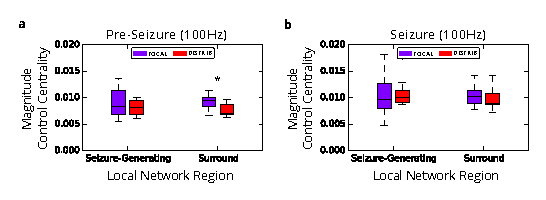
\includegraphics[width=\textwidth]{panel4.eps}
    \caption[Control centrality of surrounding network structures]{\textbf{Control centrality in surrounding network differentiates seizure type.} (\textbf{A}) Control centrality in the \textit{pre-seizure epoch} estimated within the seizure-generating area and within the surrounding tissue for partial seizures that remain focal ($N=19$) and that generalize to surrounding tissue ($N=16$): (rank-sum test; $p_\text{sz-gen}=6.8\times10^{-1}$, $p_\text{surround}=3.2\times10^{-3}$). Control centrality of the surrounding tissue is greater in the focal as opposed to the distributed epileptic networks. (\textbf{B}) Control centrality in the \textit{seizure epoch} estimated within the seizure-generating area and within the surrounding tissue for partial seizures that remain focal ($N=19$) and that generalize to surrounding tissue ($N=16$): (rank-sum test; $p_\text{sz-gen}=4.3\times10^{-1}$, $p_\text{surround}=2.4\times10^{-1}$); $p$-values are computed using a non-parametric Wilcoxon rank-sum test to account for uneven sample sizes across different seizure types. (\textbf{C}) Control centrality of desynchronizing nodes in the tissue surrounding the seizure generating area in both partial seizures that remain focal ($N=19$) and those that generalize to surrounding tissue ($N=16$): (FDA; $p_\text{pre-seizure}=9.2\times10^{-4}$, $p_\text{seizure}=2.9\times10^{-1}$). During the pre-seizure epoch, we observe significantly greater control centrality of desynchronizing nodes in partial seizures that remain focal \emph{versus} those that generalize to surrounding tissue. (\textbf{D}) Control centrality of synchronizing nodes in the tissue surrounding the seizure generating area in both partial seizures that remain focal ($N=19$) and those that generalize to surrounding tissue ($N=16$): (FDA; $p_\text{pre-seizure}=2.5\times10^{-2}$, $p_\text{seizure}=9.2\times10^{-1}$). During the pre-seizure epoch, we observe significantly greater control centrality of desynchronizing nodes in partial seizures that remain focal \emph{versus} those that generalize to surrounding tissue. \label{ch5:fig4}}
\end{figure}

Which type of putative control node (synchronizing or desynchronizing) plays a more prominent role in partial seizures that remain focal versus those that generalize to surrounding tissue? In pre-seizure epochs, we observed significantly stronger control centrality of both desynchronizing (\textbf{Fig.~\ref{ch5:fig4}C}) and synchronizing (\textbf{Fig.~\ref{ch5:fig4}D}) nodes in the focal compared to the distributed epileptic networks. Thus, both types of putative control nodes played a more prominent role in partial seizures that remained focal versus those that generalized to surrounding tissue. This suggests that focal epileptic networks exert a push-pull control mechanism to constrain seizure evolution. Note that this observation is specific to pre-seizure epochs: no differences were observed in synchronizing or desynchronizing control centrality during seizure epochs.

\section{Discussion}

In this work we asked, ``Is there a network-level control mechanism that regulates seizure evolution?'' To answer this question, we designed and applied a novel computational tool -- \emph{virtual cortical resection} -- to predict network response to removing regions in the epileptic network. Our work supports the notion that a regulatory system located outside the seizure-generating area consists of synchronizing and desynchronizing nodes, which constrain seizure evolution using an antagonistic, push-pull control mechanism.

\subsection{Spatial Extent of Seizure Evolution}
The spatial extent of the epileptic network driving seizure dynamics has been elusive. Epilepsy experts conventionally implicate the seizure-generating region as the underlying source of network dysfunction, and the surrounding irritative zone as a secondary site of abnormality that is not itself capable of independently generating seizures \cite{rosenow2001presurgical, nair2004critical}. Others have identified strong, tightly connected network hubs localized in areas outside the seizure-generating region that indicate a wider extent of network damage \cite{schevon2007cortical, zaveri2009localization-related, rummel2013systems-level}. Our results support the view that tissue surrounding the seizure-generating area displays abnormalities that support seizure evolution. Specifically, we observe the presence of putative control nodes within a broader heterogeneous network that may serve to discourage seizure spread by limiting synchronizability of healthy activity states. 

These findings may also have important neurobiological implications for epilepsy research. They raise questions such as, "What is the neuroanatomical substrate for network nodes that drive or contain seizures?" Might there be direct anatomical dysfunction such as loss of inhibiting inter-neurons, aberrant fiber-sprouting or changes in local gap junctions or ion channel expression that correlate with desynchronizing or synchronizing functional regions? Relating correlates of dysfunction from node resection and electrophysiologic studies to underlying neuroanatomy in applications of targeted drug-delivery remains a promising area of epilepsy research. 


\subsection{Push-Pull Control as a Regulatory Mechanism}
Controllability of functional brain networks is a burgeoning area of network neuroscience, particularly in the study of large-scale brain areas and the distributed circuits they constitute \cite{bassett2006adaptive, gu2014controllability}. However, these principles may have even greater impact in meso-scale brain networks, where local neural populations frequently switch between a wide variety of normal and abnormal rhythmic neural processes. Using virtual cortical resection, we observed the presence of specific nodes whose placement in the wider network suggests their critical role in controlling synchronization and desynchronization in seizure dynamics. These key areas display antithetical potential for controlling activity dynamics, and therefore we speculate that they may employ an antagonistic, push-pull control mechanism similar to that described in theoretical work in other systems \cite{he2014control}. Mechanistically, synchronizing controllers might pull the network towards a particular stable state, and, conversely, desynchronizing controllers might push the network away from the stable state. Such a mechanism also aligns with the recently proposed Epileptor model of seizure dynamics, where any brain network might be capable of seizure generation depending on its vulnerability to crossing a critical separatrix barrier \cite{jirsa2014nature, naze2015computational}. In the framework of the Epileptor, our results suggest that synchronizing and desynchronizing nodes might regulate a critical level of network stability and prevent the extent to which the network crosses a separatrix. 


\subsection{Methodological Limitations and Extensions}

An important clinical consideration related to this work is the sampling error inherent in any intracranial implantation procedure. Any of the techniques used to map epileptic brain usually yield incomplete representations of the epileptic network. It is not possible to fully record from the entirety of cortex in affected patients. In some cases this might mean that neither seizure onset zones nor all regions of seizure spread are fully delineated.

The virtual cortical resection approach can be extended to model other complex dynamics beyond independent node contributions to network synchronization. For example, we could iterate over all possible node resections to find the network configuration that optimizes synchronizability. Furthermore, in this work we apply virtual cortical resection to study a single topological metric, network synchronizability. Additional quantities of interest include measures of causal information flow \cite{korzeniewska2014ictal}.

\subsection{Clinical Impact}
Isolating the natural control mechanisms of brain function is critical for clinical translation. Enhancing and disrupting these natural control mechanisms could be a viable approach for introducing therapy with implantable devices for network disorders like epilepsy. Current methods of treating drug-resistant epilepsy rely on surgical resection or, more recently, implantable devices. However, predicting network response to therapy remains challenging. The virtual cortical resection technique is a novel, objective method of probing robustness and fragility upon removing components of the epileptic network. Using this method, we pinpointed putative network controllers that may be crucial for seizure evolution -- suggesting that resection of these regions may compromise key mechanisms to contain seizure activity.

This technique will require careful retrospective, and perhaps eventually prospective, trials to validate its utility. There are frequent examples of patients in whom seizures appear to be localized on intracranial EEG who go on to have recurrent or persistent seizures despite surgical resection or device placement. It is our hope that practical implementations of models like our virtual cortical resection may allow clinicians to predict response to therapy and provide a quantitative guide to what is now a process guided by manual interpretation of ECoG recordings. 

There may also be clinical implications beyond just guiding electrode placement for anti-epileptic devices. These studies might open the way towards more accurate electrophysiologically-guided cortical resection or perhaps pinpointed thermal ablation to specific network regions, similar to procedures done by cardiac electrophysiologists. These potential applications, while far off, offer considerable clinical advantage over the large cortical resections performed currently, with modest seizure-freedom rates.  

\section{Methods}
\subsection{Patient Data Sets}
\subsubsection{Ethics Statement}
All patients included in this study gave written informed consent in accordance with the Institutional Review Board of the University of Pennsylvania.

\subsubsection{Electrophysiology Recordings}
Ten patients undergoing surgical treatment for medically refractory epilepsy believed to be of neocortical origin underwent implantation of subdural electrodes to localize the seizure onset zone after presurgical evaluation with scalp EEG recording of ictal epochs, MRI, PET and neuropsychological testing suggested that focal cortical resection may be a therapeutic option. Patients were then deemed candidates for implantation of intracranial electrodes to better define epileptic networks. De-identified patient data was retrieved from the online International Epilepsy Electrophysiology Portal (IEEG Portal) \cite{wagenaar2013multimodal}.

ECoG signals were recorded and digitized at 500 Hz sampling rate using Nicolet C64 amplifiers and pre-processed to eliminate line noise. Cortical surface electrode (Ad Tech Medical Instruments, Racine, WI) configurations, determined by a multidisciplinary team of neurologists and neurosurgeons, consisted of linear and two-dimensional arrays (2.3 mm diameter with 10 mm inter-contact spacing) and sampled the neocortex for epileptic foci (depth electrodes were first verified as being outside the seizure onset zone and subsequently discarded from this analysis). Signals were recorded using a referential montage with the reference electrode, chosen by the clinical team, distant to the site of seizure onset and spanned the duration of a patient's stay in the epilepsy monitoring unit. See Table 1 for demographic and clinical information.

\begin{table}[H]
    \scriptsize
    \centering
    \begin{tabular}{|x{2cm}|x{0.5cm}|x{0.75cm}|x{2cm}|x{1.5cm}|x{1.25cm}|x{1cm}|x{1cm}|x{1.40cm}|}
        \hline
        Patient\newline (IEEG Portal) & Sex & Age & Seizure Onset & Etiology & Seizure Type (N) & Imaging & Outcome \\ \hline \hline
        \verb|HUP64_phaseII| & M & 03/20 & Left frontal & Dysplasia & CP+GTC (1) & L & I\\ \hline
        \verb|HUP65_phaseII| & M & 02/36 & Right temporal & Auditory reflex & CP+GTC (3) & N/A & I\\ \hline
        \verb|HUP68_phaseII| & F & 15/26 & Right temporal & Meningitis & CP (1), CP+GTC (4) & NL & I\\ \hline
        \verb|HUP70_phaseII| & M & 10/32 & Left perirolandic & Cryptogenic & SP (8) & L & NR\\ \hline
        \verb|HUP72_phaseII| & F & 11/27 & Bilateral left & Mesial temporal sclerosis & CP+GTC (1) & L & NR\\ \hline
        \verb|HUP73_phaseII| & M & 11/39 & Anterior right frontal & Meningitis & CP+GTC (5) & NL & I\\ \hline
        \verb|HUP78_phaseII| & M & 00/54 & Anterior left temporal & Traumatic injury & CP (5) & L & III\\ \hline
        \verb|HUP79_phaseII| & F & 11/39 & Occipital & Meningitis & CP (3) & L & NR\\ \hline
        \verb|HUP86_phaseII| & F & 18/25 & Left temporal & Cryptogenic & CP+GTC (2) & NL & II\\ \hline
        \verb|HUP87_phaseII| & M & 21/24 & Frontal & Meningitis & CP (2) & L & I\\ \hline
    \end{tabular}
    \caption[Patient data set for Chapter \ref{ch:selfreg}]{\textbf{Patient information.} Patient data sets accessed through IEEG Portal (http://www.ieeg.org). Age at first reported onset and at phase II monitoring. Localization of seizure onset and etiology is clinically-determined through medical history, imaging, and long-term invasive monitoring. Seizure types are SP (simple-partial), CP (complex-partial), CP+GTC (complex-partial with secondary generalization). Counted seizures were recorded in the epilepsy monitoring unit. Clinical imaging analysis concludes L, Lesion; NL, non-lesion. Surgical outcome was based on Engel score (scale: I-IV, seizure freedom to no improvement; NR, no-resection; NF, no follow-up). M, male; F, female. \label{ch5:tab1}}
\end{table}

\subsubsection{Description of Epileptic Events}
We analyzed 19 partial seizures (simple and complex) and 16 partial seizures that generalized to surrounding tissue, forming a population of focal and distributed epileptic networks, respectively. Seizure type, onset time, and onset localization were marked as a part of routine clinical workup.

The seizure state spanned the period between clinically-marked earliest electrographic change (EEC) \cite{litt2001epileptic} and termination; and the pre-seizure state spanned a period equal in duration to the seizure state and ended immediately prior to the EEC (we refer to each pair of pre-seizure and seizure states as an \textit{event}).

\subsection{Functional Network Construction}
\subsubsection{Pre-Processing}
ECoG signals from each event were divided into 1-second, non-overlapping, wide-sense stationary time-windows in accord with related studies \cite{kramer2010coalescence}. In each time window, signals were re-referenced to the common average reference \cite{kramer2010coalescence, towle1999electrocorticographic} to account for variation in reference location across patients and to avoid broad field effects that may bias connectivity measurements erroneously in the positive direction.

\subsubsection{Coherence Estimation}
We constructed functional networks in each time-window using multitaper coherence estimation, which defines a network connection between electrode pairs as the power spectral similarity of signal activity over a specific frequency band. We applied the \textit{mtspec} Python implementation \cite{prieto2009fortran} of multitaper coherence estimation with time-bandwidth product of 5 and 8 tapers in accord with related studies \cite{kramer2011emergence}. Based on vast literature implicating high-frequency oscillations and $\gamma$ activity as drivers of epileptic activity, we primarily studied functional connectivity in the high-$\gamma$ band (95--105 Hz). This frequency range represents relatively local neural population dynamics that are largely unaffected by volume conduction.

\subsection{Metrics of the Time-Varying Functional Network}

\subsubsection{Network Geometry}
In our network analysis, we refer to heterogeneity of network architecture in the context of node strength, also known as weighted degree. We measure a time-varying quantity of heterogeneity: the dispersion of the degree distribution in each time window. We use a non-parametric, interquartile distance measure to quantify dispersion. The interquartile distance is the 75th percentile subtracted by the 25th percentile of a distribution.

\subsubsection{Network Synchronizability}
A recent trend in studying functional networks is to model dynamic geometric structure that evolves through states \cite{wulsin2013parsing, rummel2013systems-level, burns2014network}. Building on the classical notion of stability of the synchronized state in static networks, we fit a popular synchronizability model for dynamic networks \cite{gomez2013diffusion} to account for time-varying structure of the functional networks in our study. As a simplification for our analysis, we assume functional networks between time-windows are independent.

To quantify synchronizability, we first estimated the time-varying Laplacian matrix $\textbf{L}(t)$ for each time-window $t$ of the functional network. Intuitively, each entry $l_{ij}(t)$ of $\textbf{L}(t)$ quantifies how easily information could diffuse between nodes $i$ and $j$ based on the relative connectivities of both nodes to all other nodes in the network. Next, we computed the eigenspectrum of $\textbf{L}(t)$ and calculated the ratio of the second-smallest eigenvalue $\lambda_2$ to the largest eigenvalue $\lambda_\text{max}$ for each $t$, resulting in network synchronizability $s_{t}=\frac{\lambda_2}{\lambda_\text{max}}$ (larger values of $s(t)$ correspond to greater state stability) \cite{barahona2002synchronization}. The \textbf{Supplementary Note} provides details of the \textit{master stability function} formalism behind synchronizability and its relationship to state stability. 

\subsubsection{Virtual Cortical Resection}
To model potential effects of resecting or lesioning regions of brain networks, we develop a virtual cortical resection technique. Generally, the approach allows us to ask how network topology might change upon removing one or more nodes or connections in the network. In time-varying networks, virtual cortical resections may be useful in patterned lesioning schemes for implantable devices that continuously modulate brain state away from seizures \cite{stanslaski2012design, afshar2013translational}.

Here, we tailored virtual cortical resection to study putative controllers that regulate synchronizability in the epileptic network. We measure the control centrality, the contribution of a node to network synchronizability, by applying virtual cortical resection to each node in each time-window of the functional network. The control centrality identifies a node as a desynchronizing ($c_i > 0$) or synchronizing ($c_i < 0$) controller. The \textbf{Supplementary Material} explores the relationship between control centrality and other topological properties of networks.

\subsubsection{Statistical analysis}
We compared time-varying network metrics between partial seizures that remain focal and partial seizures that generalize to surrounding tissue. We performed this comparison by (i) normalizing each seizure event into 20 sequential time-bins spanning the pre-seizure and seizure states and (ii) employing functional curve analysis to statistically test differences in temporal dynamics between seizure type, independently in each state. We assigned $p$-values to each state by re-assigning events uniformly at random to seizure types up to 1,000,000 times and computing the mean area between the resulting functional curves.

\section{Acknowledgments}
AK and BL acknowledge support from the National Institutes of Health through awards \#R01-NS063039, \#1U24 NS 63930-01A1, the Citizens United for Research in Epilepsy (CURE) through Julie's Hope Award, and the Mirowski Foundation. DSB acknowledges support from the John D. and Catherine T. MacArthur Foundation, the Alfred P. Sloan Foundation, the Army Research Laboratory, the Institute for Translational Medicine and Therapeautics, the National Institute of Mental Health through award number 2-R01-DC-009209-11 (Thompson-Schill), and the National Science Foundation awards CRCNS BCS-1441502 and BCS-1430087 through the ENG, CISE, and SBE directorates. The content is solely the responsibility of the authors and does not necessarily represent the official views of any of the funding agencies.

\section{Supplemental Information}
\subsection{Master Stability Function for Network Synchronizability}
The traditional notion of connectivity in brain networks is the statistical relationships between cortical regions and how such relationships change with time \cite{friston2011functional, hutchison2013dynamic}. In addition to describing topology, connectivity can be used to query how neural processes at each node diffuse along pathways between cortical areas. The latter study of network organization asks the nature of diffusive dynamics on static or time-varying networks. 

Modeling diffusion of processes over the network is critical for asking pertinent questions in neuroscience more generally and epilepsy more specifically, such as "How does brain activity synchronize during seizures?" As functional brain networks re-organize, the ability for neural processes at each node to synchronize also changes, a property known as \textit{synchronizability} \cite{barahona2002synchronization}. These attributes are captured by a generative model for diffusion over the networks, called the \textit{master stability function} \cite{pecora1998master, gomez2013diffusion} -- defined as:
\begin{equation}\label{masterstab}
    \dot{x_i}(t) = f(x_i(t)) + \sigma(t)\sum\limits_{j=1}^{N}A_{ij}(t)(x_j(t) - x_i(t))
\end{equation}
where $x_i(t)$ represents the dynamical state of node $i$, $f$ is a function describing independent node dynamics, $\sigma$ is a diffusion constant, $A(t)$ is an $N \times N$ adjacency matrix of connection weights between $N$ network nodes. For a time-varying functional network, where each time window is assumed independent, the solution of Eqn. (\ref{masterstab}) is given by:
\begin{equation}\label{lapl}
    \dot{x}(t) = -\mathcal{L}(t)x(t)
\end{equation}
where $\mathcal{L}$ is the graph Laplacian whose entries $l_{ij}$ quantify how easily neural processes can diffuse between nodes $i$ and $j$. For a given network configuration, the potential for dynamics at each node to achieve equivalence around a state $q(t)$ such that $q(t)=x_1(t)=x_2(t)=...=x_N(t)$ is the network synchronizability $s(t)$. The stability of the synchronized state $q(t)$ is quantified by the eigenvalues of $\mathcal{L}$ such that:
\begin{equation}\label{sync}
    s(t) = \frac{\lambda_2}{\lambda_\text{max}}
\end{equation}
where $\lambda_2$ and $\lambda_\text{max}$ are the second-smallest and largest eigenvalues, respectively. Larger values of $s(t)$ correspond to greater potential for the network to stably synchronize.   

\subsection{Virtual Cortical Resection}
In the previous subsection we explored methods to query how easily diffusion dynamics on a network can synchronize. Synchronizability is governed by network organization, and as the network reconfigures over time so does its potential to synchronize. In this work we ask a non-trivial question regarding network synchronizability, "Which nodes are most important controllers for regulating synchronizability?" Answering this question may have significant impact in understanding which regions of the network naturally maintain stability in the synchronized state.

Our approach was to independently remove network regions (virtual cortical resection) and measure change in the ability of the modified network to stably synchronize. The removed region was assigned a control centrality equal to the fractional change in synchronizability in the modified network from the original network. Based on the relative increase or decrease of synchronizability, we found that individual nodes can assist in stabilizing the synchronized state by either desynchronizing or synchronizing the network. 

Importantly, we investigated whether control centrality is an emergent property of network topology or simply related to the average strength of connections from that node. To this end, we computed the amount of variance in control centrality that is explained by nodal strength during the pre-seizure and seizure epochs in the example focal (\textbf{Fig.~\ref{ch5:figS1}A}) and distributed epileptic networks (\textbf{Fig.~\ref{ch5:figS1}B}). In both events we observed low linear relationships between control centrality and degree centrality in the pre-seizure and seizure epochs. These results suggest control centrality is a novel measure of network geometry specifically related to the synchronization of dynamic processes.   

\begin{figure}[H]
    \centering
    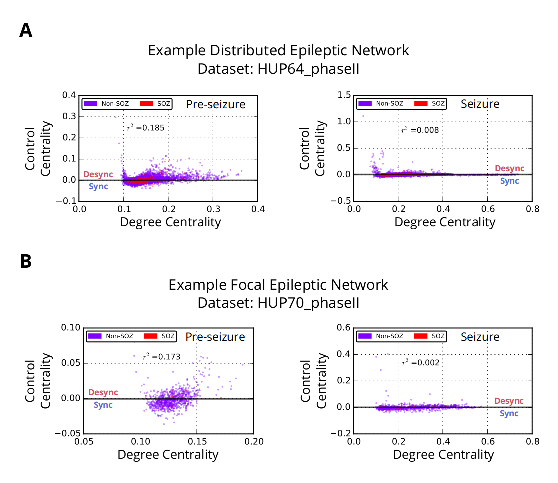
\includegraphics[width=\textwidth]{panelS1.eps}
    \caption[Control centrality as a network measure]{\textbf{Control centrality as a network measure.} (\textbf{A}) Relationship between control centrality and weighted degree centrality over all time-windows during pre-seizure (\textit{left}) and seizure (\textit{right}) epochs in a sample event from the \textit{distributed epileptic network}. (\textbf{B}) Relationship between control centrality and weighted degree centrality over all time-windows during pre-seizure (\textit{left}) and seizure (\textit{right}) epochs in a sample event from the \textit{focal epileptic network}. $r^2$ measures the amount of variance in control centrality explained by weighted degree centrality. \label{ch5:figS1}}
\end{figure}
		
			
\chapter{Conclusions and Discussion}
\label{ch:conclusion}

% the code below specifies where the figures are stored
\ifpdf
    \graphicspath{{conclusion/figures/PNG/}{conclusion/figures/PDF/}{conclusion/figures/}}
\else
    \graphicspath{{conclusion/figures/EPS/}{conclusion/figures/}}
\fi

% ----------------------------------------------------------------------
%: ----------------------- conclusion content ----------------------- 
% ----------------------------------------------------------------------

\section{Contributions}
In this thesis, we modeled functional networks of epileptic neocortex in human patients and studied functional pathways that drive the generation, propagation, and termination of seizures. The primary goal of this thesis was to characterize epilepsy as a network disorder of dysfunctional brain circuitry by abstracting beyond current clinical practice of localizing isolated islands of pathologic cortical tissue. Addressing this goal might relieve the clinical burden of identifying targets for surgical intervention, which in many cases leads to little reduction in a patient's seizures, and may pave the road for integrating novel neurotechnologies capable of controlling network dysfunction into clinical practice. To this end, we developed and applied graph theoretic and machine learning algorithms for objectively mapping functional network pathways between distributed cortical structures related to conventional clinically-defined targets. 

In Chapter \ref{ch:netdrivers}, we modeled time-varying functional connectivity of the epileptic network and applied a novel community detection algorithm for clustering patterns of connection geometry into discrete, time-dependent network states preceding and during seizures. We found that the network states corresponded to stages of seizure generation, propagation and termination and connections between cortical structures in the seizure-onset zone are persistently stronger than all other network connections. Results from these investigations suggest that clustering time-varying network architecture can parse seizures and robustly pinpoint seizure-onset regions, potentially improving the inter-rater reliability currently hindering interpretation of electrophysiology from patients with neocortical epilepsy.

In Chapter \ref{ch:mapsubnet}, we disentangled modular sub-networks from time-varying functional connectivity and applied an ensemble clustering technique for quantifying similarity of cortical pathways engaged during seizures and normal, interictal periods. We found that functional connections of the epileptic network form cohesive, stable sub-networks that are expressed during seizures and recapitulated during interictal periods. These sub-networks form clusters that reliably predict functional pathways incorporating clinically-defined seizure-onset regions. Secondly, we find that functional sub-networks are persistently expressed during interictal periods and more transiently expressed during seizures. Our findings have clinical implications in delineating sub-networks generating seizures during interictal periods, many hours prior to seizure onset.

In Chapter \ref{ch:selfreg}, we developed a simulation technique for conducting virtual resections on regions of the epileptic network and applied the approach to a data set of two types of seizures, those that spread over cortex and others that remain contained to a local cortical region. We found that specific network controllers in cortical regions outside clinically-defined seizure onset nodes, regulate the future spread of seizures. These findings suggest network regions outside of conventional clinical targets regulate seizure spread, suggesting the epileptic network is more complex and distributed than originally believed.

Taken together, this thesis work demonstrated that functional connectivity derived from activity of neural populations at millimeter scale explains, at least in part, functional architecture of the epileptic network. Our findings suggested that regions generating seizures exhibit stereotyped patterns of connectivity, which may be predicted many hours before epileptic events. Finally, we generated a notion of network stability that may be used for probing cortical controllers of seizure evolution.

\section{Future Studies}
While this work yields many insights regarding the architecture of the epileptic network, clinical translation of these tools requires further validation. Many of the network properties studied in this thesis were related back to ``gold-standard'' markings of seizure-onset regions in a data set of highly varying patient outcome. This poses several problems: (i) a consensus definition of seizure-onset is lacking and unreliable across clinicians and institutions, (ii) well-defined seizure-onset may still lead to poor outcome, and (iii) resection margins may only partially overlap with the seizure-onset region.

To reliably validate objective algorithms for mapping dysfunction in epileptic networks, we should differentiate functional connectivity within the resection zone of patients who experienced good and bad seizure reduction. This study would enable a more direct comparison of network architecture with a variable closest to seizure reduction. We hypothesize that spatially distributed, strongly connected nodes, which significantly corresponded to cortical structures within seizure-onset zone, may have a large overlap with resected nodes in patients with good outcome. Alternatively, we can test whether resecting controllers in regions outside the seizure-onset nodes leads to better containment of seizure activity -- verifying the utility of the developed virtual cortical resection technique. 

Along a similar line of thought, we speculate that network architecture may predict post-surgical seizure freedom. In patients with seizures generated near network hubs connecting many distributed cortical structures, we hypothesize resective surgery may not lead to favorable outcome. To test this hypothesis, we could use linear mixed effects models to stratify clinical scales of seizure freedom (Engel or ILAE) based upon network measures such as stability (synchronizability), number of sub-networks, or spatial extent of strongest connections. These studies can have potential clinical impact in screening patients who are good candidates for resective surgery.

Another line of work that requires validation is using functional architecture of the epileptic network to pinpoint stimulation targets for implantable devices. We hypothesize that functional connections within the network can be leveraged to deliver stimulation to specific cortical structures. Testing this hypothesis might involve tracking the effects of stimulation on functional architecture to predict whether stimulating at one node results in changes in neural activity at a connected node. We can then assess whether stimulating nodes with connections leading to seizure-onset areas might abort seizure evolution.

All facets of this important future work will be essential for introducing the findings of this dissertation into clinical practice. 
  

% --------------------------------------------------------------
%:                  BACK MATTER: appendices, refs,..
% --------------------------------------------------------------

%: ----------------------- Appendicies ------------------------
%\begin{partChapter}
%
\begin{appendices}
\chapter{Some Appendix}
\lipsum
\section{first section}
\lipsum
\chapter{Another Appendix}
\lipsum
\end{appendices}

%\end{partChapter}

% --------------------------------------------------------------
% backmatter mode set after appendix 
% any chapters beyond here have chapter number supressed
% --------------------------------------------------------------

\backmatter

%: ----------------------- glossary ------------------------

% Tie in external source file for definitions: /backmatter/glossary.tex
% Glossary entries can also be defined in the main text. See glossary.tex
%% this file is called up by thesis.tex
% content in this file will be fed into the main document

% Glossary entries are defined with the command \nomenclature{1}{2}
% 1 = Entry name, e.g. abbreviation; 2 = Explanation
% You can place all explanations in this separate file or declare them in the middle of the text. Either way they will be collected in the glossary.

% required to print nomenclature name to page header
\markboth{\MakeUppercase{\nomname}}{\MakeUppercase{\nomname}}


% ----------------------- contents from here ------------------------

\nomenclature[Xe ]{11HUGS}{11 Mpc Halpha and Ultraviolet Galaxy Survey} 
\nomenclature[Zt ]{2MASS}{Two-Micron All Sky Sruvey}
\nomenclature[Am ]{M}{Mass of object}
\nomenclature[Gm ]{$\tau$}{Optical depth}
\nomenclature[Rs ]{$\ ^{*}$}{Conjugate}
\nomenclature[Ss ]{$\astrosun$}{relating to the sun (Sol)}
 

%\clearpage
%\begin{partChapter}
%\begin{multicols}{2} % \begin{multicols}{#columns}[header text][space]
%\begin{footnotesize} % scriptsize(7) < footnotesize(8) < small (9) < normal(10)

%\printnomenclature[1.5cm] % [] = distance between entry and description
%\label{nom} % target name for links to glossary

%\end{footnotesize}
%\end{multicols}
%\end{partChapter}


% --------------------------------------------------------------
%: ----------------------- bibliography ------------------------
% --------------------------------------------------------------
% Various bibliography styles exist. Replace style as desired.

% For the following 4 bibliography styles:
% in-text refs: (1) (1; 2)
% ref list: alphabetical; author(s) in small caps; initials last name; page(s)
% PhDbiblio-case = title forced lower case
% PhDbiblio-bold = title as in bibtex but bold
% PhDbiblio-url = bold + www link if provided
% PhDbiblio-url2 = names small caps, title bold & hyperlinked, link to page 
% PhDbiblio-intext-twoauth= similar to PhDBiblio, with intext author citations 

% jmb = calls style file jmb
% in-text refs: author (year) without brackets
% ref list: alphabetical; author(s) in normal font; last name, initials; page(s)

%\bibliographystyle{plainnat} % calls style file plainnat.bst
% in-text refs: author (year) without brackets
% (this works with package natbib)
% --------------------------------------------------------------

\clearpage
%\begin{partChapter}
%\begin{multicols}{1} % \begin{multicols}{ # columns}[ header text][ space]
\begin{footnotesize} % tiny(5) < scriptsize(7) < footnotesize(8) < small (9)

\bibliographystyle{Latex/Classes/PhDbiblio-url} % Title is link if provided
\renewcommand{\bibname}{References} % changes the header; default: Bibliography

\bibliography{./backmatter/references} % adjust this to fit your BibTex file

\end{footnotesize}
%\end{multicols}
%\end{partChapter}



%: ----------------------- Index ------------------------
%\clearpage
%\begin{partChapter}
%\printindex
%\end{partChapter}


%: --------------------------------------------------------------
%:                     END OF DOCUMENT!!!
% --------------------------------------------------------------
\end{document}
